\documentclass[11pt,a4paper]{article}
\usepackage[a4paper,margin=0.8in]{geometry}
\usepackage{amsmath,amssymb}
\usepackage{booktabs,graphicx,longtable}
\usepackage{amsthm,enumitem,xr}
\usepackage[round,authoryear]{natbib}
\usepackage[hidelinks]{hyperref}
\externaldocument{eesp_cor}
\newtheorem{theorem}{Theorem}
\newtheorem{proposition}{Proposition}
\newtheorem{lemma}{Lemma}
\newtheorem{assumption}{Assumption}
\renewcommand{\thetheorem}{S\arabic{theorem}}
\renewcommand{\theproposition}{S\arabic{proposition}}
\renewcommand{\thelemma}{S\arabic{lemma}}
\renewcommand{\theassumption}{S\arabic{assumption}}
\renewcommand{\theequation}{S\arabic{equation}}
\DeclareMathOperator*{\argmin}{arg\,min}
\newcommand{\E}{\mathbb{E}}
\renewcommand{\Pr}{\mathbb{P}}
\newcommand{\R}{\mathbb{R}}
\newcommand{\one}{\mathbf{1}}
\newcommand{\Dn}{\mathcal{D}_n}
\newcommand{\appref}[1]{\ref{#1}}
\renewcommand{\thetable}{S\arabic{table}}
\renewcommand{\thefigure}{S\arabic{figure}}
\title{Supplement to ``Group recovery after trimming, and level-free flagging,\\ in robust clusterwise regression''}
\author{Samir Orujov}
\date{}
\begin{document}
\maketitle

\section*{S0 Contents}

Throughout, \emph{ESF} is the exact-subsample flagging procedure of Algorithm~1 of the paper,
followed by the recovery step of Algorithm~2 unless ``ESF alone'' is written; ``reweighted''
or ``rw'' is the reweighting rule of the paper (Section~3 of the paper, applied twice,
$c=2.5$, a median absolute deviation per group); TCLUST-REG$^{\ast}$ denotes TCLUST-REG with
$5\%$ second trimming in the covariates. The analysis plans, the code, the raw results and the
exact job scripts are in the repository \url{https://github.com/sorujov/eesp}.

\begin{center}\small
\begin{tabular}{lp{11.5cm}}
\toprule
Section & Contents \\
\midrule
S1 & Software and settings of the competitors \\
S2 & Proofs of the results of Section~3 of the paper: the precise form of Proposition~1 and the vote within one stage (S2.0, S2.1), Theorems~S1 and~S2, the precise form of Proposition~2 and its scope (S2.2), the precise form of Proposition~3 and the local peak test (S2.3) \\
S3 & Tables S1 to S29: the comparison of Plan~1 cell by cell for ESF alone (S1); the vote weight $\lambda$ (S2); the cut-off $c$ and the covariate quantile (S3); every method in every design and at every fraction of outliers, with Monte Carlo standard errors (S4 to S11); the subsample size $m$ (S12); the loss cap $c_{\mathrm b}$ (S13); ablation of the exact fit (S14); a single $m=12$ (S15); composition of the flagged set (S16); the recovery step after TCLUST-REG (S17); choice of $K$ (S18); coefficient error (S19); flagged fraction of the methods that estimate it (S20); mixtures with more starts (S21); cost of the branch and bound (S22); sensitivity of the recovery step (S23); the best-of-five rule (S24); the third part cell by cell (S25); solvers at further sizes (S26); mixtures started from least squares (S27); small-group designs with $m=12$ (S28); $B=500$ (S29) \\
S4 & Exact solvers for the subsample problem, with Table S30 \\
S5 & Further tables of Section~4 of the paper: mean flagged fraction (S31), computing times (S32), Plan~5 (S33); detail of Sections~4 and~5 of the paper (S5.1); analysis plans and digests (S34); tone perception data (S35); confirmation of the recovery step under Plan~3 (S36); worst-case summaries with the settings first planned (S37, S38); further competitors and checks (S39); long-search TCLUST-REG cell by cell (S40); the fresh data of Plan~4 (S41) \\
S6 & Other settings of TCLUST-REG (S6.1), further competitors and checks (S6.2), the loss cap, repeated runs and the best-of-five rule (S6.3), the third part of the study in detail (S6.4), and, in S6.5, the fishery figure (Figure S1), the fishery and taxi tables (S42, S43) and the table of constants (S44); the adjusted Rand index on all units (S45); the recovery step after the trimmed cluster-weighted model (S46); the analysis plans (S47); the noise range of the recovery step (S48); TCLUST-REG's own assignment (S49); the deciding cells with $200$ data sets (S50) \\
S7 & Implementation of ESF: the exact subsample fit, alignment and vote, concentration steps, software \\
\bottomrule
\end{tabular}
\end{center}

Tables~S4--S11 give, for every design, the mean accuracy on clean units of every method at every
fraction of outliers, with Monte Carlo standard errors. Columns $0.00$--$0.20$ come from the
first part of the study ($50$ data sets per cell), columns $0.25$--$0.35$ from the second part
($100$ data sets per cell, new data); the column ``$0.30$ (part 1)'' repeats $\varepsilon=0.30$ from
the first part, which lay outside the criteria of Plan~1. The Laplace, contaminated normal and
noise-component mixtures, added after Plan~1, appear in Tables~S4--S11 but not in Table~S1.
``Trimmed alternation'' is a simple trimmed least-squares alternation with the reweighting step,
given the computing time of ESF alone without the covariate screen; it is reported for
completeness only. A failed fit counts as accuracy $0$; CTLE failed on $63$ of the $2{,}000$ data
sets of the first part and $154$ of the $2{,}400$ of the second; TLE failed in $16$ and $22$ fits
over all its levels, and the bisquare mixture in $8$ and $2$.

\paragraph{Analysis plans.} Each plan was written as a plain-text file before the data it
concerns were analysed (Plans~1 and 2) or generated (Plans~3 to 5), and served to fix the
comparison and its thresholds before the run: Plan~1 for the first part, Plan~2 for the
second, Plans~3 and~4 for the recovery step, on the stored fits and on $600$ fresh data sets,
and Plan~5 for three designs outside the Gaussian family; the third part is descriptive
(Table~\ref{tab:plans}). Table~\ref{tab:prereg} gives the SHA-256 digest
of each file as frozen;
the files in the repository reproduce these digests. The file of Plan~5 carries one line added
after freezing, which records that the code differs from that of Plan~4 only by an optional
argument not used by the plan; the digest is that of the file without this line. Plans~3 to 5
also record the digests of the code they fix. The plans document what was fixed when; the main
rival pipeline of the paper (long-search TCLUST-REG with reweighting and the recovery step),
the three mixtures and sequential RANSAC, the best-of-five rule and the guard in the scoring
scale were decided after all of them.


\section*{S1 Software and settings of the competitors}
\label{supp:software}

TCLUST-REG is the function \texttt{tclustreg} of the FSDA toolbox, a MATLAB toolbox. We ran it
unmodified (GitHub commit \texttt{37f998e} of 24 September 2026) under GNU Octave~9.4 with the
\texttt{statistics} package ($1.6.7$ for the simulations, $1.6.3$ for the data of Section~5),
with three one-line substitutes for MATLAB functions that Octave lacks: a version check that
returns false, \texttt{coder.target}, which returns true for \texttt{"MATLAB"}, and
\texttt{convertStringsToChars}, which returns its arguments; they are in the repository. The runs
with adaptive second-level trimming (Section~S6) needed a fourth, for
\texttt{any(x,'all')}, which Octave's \texttt{any} does not accept.

TCLUST-REG was then run again in MATLAB (R2026a Update~5 in MATLAB Online, FSDA at the same
commit, no substitutes) on $80$ data sets, ten replications of each of the eight design cells of
Table~\ref{tab:matlab}, each at both levels with $1000$ starts and $50$ refinement steps. MATLAB's
random number generator differs from Octave's, so the two programs drew different starts. They
returned the same coefficients, to the ten significant digits both programs write and up to the
labelling of the groups, in $68$ of the $160$ fits; in the other $92$ the largest coefficient
difference exceeded $2\times10^{-3}$ of the largest coefficient. The Octave runs did not record the objective, so each fit was also scored by one criterion computed from its
coefficients: concentration steps at the fit's level with the ratio of the group variances bounded
by $12$, then the trimmed classification log-likelihood. On the MATLAB fits this score equalled
the objective that MATLAB reports to within $0.5$ in $137$ of the $160$ fits and differed from it
by up to $13$ in the rest. MATLAB's fit scored higher by more than
$0.5$ in $28$ fits and Octave's in $30$; the rest were within $0.5$. With the margin raised to $2$ the counts were $21$ and $22$, and
with $5$ they were $17$ and $12$. Neither program found better
optima more often, and the differences are those of two random searches. After reweighting and
the recovery step the mean accuracy over the $160$ fits was $0.836$ in MATLAB and $0.830$ in
Octave. Cell means differed by up to $0.09$, and by more than $0.05$ only in cells where no fit agreed. MATLAB Online took a median of $1.2$ seconds per fit and Octave, on our cluster, $41$ seconds.
The two ran on different machines, so the ratio of about $36$ mixes interpreter and hardware; the
times of TCLUST-REG in Table~\ref{tab:time}, measured on the cluster, overstate its cost in MATLAB
by a factor of that order.

The trimmed cluster-weighted model, TLE, CTLE, the bisquare mixture and the Laplace mixture come
from the R package \texttt{RobMixReg}~1.1.3; the trimmed cluster-weighted model was given $50$
random starts and $20$ concentration steps, more than its defaults, and the Laplace mixture is
\texttt{mixLp} with \texttt{nit}$=20$. The bisquare mixture \texttt{mixlinrb\_bi} raised an error
in our R session, because its single-start routine fits \texttt{lm(formula, data, weights = w)}
with a formula whose environment does not contain \texttt{w}; we ran a copy of the two package
functions in which only this line sets the formula environment first (\texttt{bisq\_patched} in
\texttt{r\_methods.R}). The computation is otherwise the package's. No package offers the contaminated normal and the
noise-component mixtures of regressions, so the implementations are ours. The contaminated
normal mixture is fitted by an ECM algorithm from $50$ starts, each from $K$ random elemental
lines with the units far from all of them starting as bad points, with the inflation started at
$20$ and the ratio of the group variances bounded by $12$; starts from random partitions, which
we tried first, were captured by the outliers. The noise-component mixture is fitted by EM from
$10$ random partitions, the best continued after $10$ iterations, with the ratio of the component
variances bounded by $12$, as in TCLUST-REG. Table~\ref{tab:S21} repeats the three mixtures with
more starts.

A simple trimmed alternation of our own at the same five levels, with the reweighting step,
completes the set that the comparison of Plan~1 used; it is a home-made
baseline, so it appears in the Supplement only, although it is the best competitor in some
cells of Table~\ref{tab:S1}.

\section*{S2 Proofs}
\label{supp:proofs}

This section proves the results of Section~3 of the paper: Proposition~\ref{prop:clean} and the guarantee for a vote within one stage (S2.0, S2.1), Proposition~\ref{thm:step} and its general version (S2.2), and Proposition~\ref{prop:recover-value} together with the result on the local peak test (S2.3). Each result is for a fixed input or fixed parameters. None covers the passage from one stage of ESF to the next, the weighted vote, or the search for the candidate line of the recovery step; the remarks that follow each proof say what it covers and what it does not.

\subsection*{S2.0 Proposition~\ref{prop:clean}: precise statement and proof}

Let $\mathcal F_{\ell-1}$ be the flagged set after stage $\ell-1$, with $\mathcal F_0$ the
covariate screen, $E_\ell=\{1,\dots,n\}\setminus\mathcal F_{\ell-1}$ the set from which stage
$\ell$ draws, $N_\ell=|E_\ell|$, $\varepsilon_\ell=|E_\ell\cap O|/N_\ell$, and $\mathcal H_{\ell-1}$ the data
together with everything drawn before stage $\ell$. A replicate of stage $\ell$ is obtained
by drawing uniform subsamples of size $m$ from $E_\ell$ until an admissible one is found; let
$q^{c}_\ell$ be the fraction of admissible subsamples among the clean subsamples of $E_\ell$,
and $q_\ell>0$ the fraction among all subsamples of $E_\ell$.

\emph{Proposition~\ref{prop:clean} (precise statement).}
Conditionally on $\mathcal H_{\ell-1}$, the subsamples of stage $\ell$ are independent, and each
is uniform on the admissible subsamples of size $m$ of $E_\ell$, however many units two of them
share. Let $p_\ell=\binom{N_\ell-|E_\ell\cap O|}{m}\big/\binom{N_\ell}{m}$ be the probability that a
uniform subsample of $E_\ell$ is clean, and $a_\ell=q^{c}_\ell/q_\ell$. Conditionally on
$\mathcal H_{\ell-1}$, each replicate of stage $\ell$ is clean with probability
$\pi_\ell=p_\ell a_\ell$, and the stage contains a clean replicate with probability
$1-(1-p_\ell a_\ell)^{B/L}$. Moreover $a_\ell\ge q^{c}_\ell$ and, when
$|E_\ell\cap O|\le N_\ell-m$,
$\{1-\varepsilon_\ell N_\ell/(N_\ell-m+1)\}^{m}\le p_\ell\le(1-\varepsilon_\ell)^{m}$.

\emph{The first statement.} Fix a replicate of stage $\ell$. Conditionally on
$\mathcal H_{\ell-1}$ its proposals are independent uniform subsamples of size $m$ of $E_\ell$,
because $E_\ell$ is determined by $\mathcal H_{\ell-1}$ and the draws use fresh randomness. (The
implementation draws $m$ units without replacement with equal weights on $E_\ell$ and zero
weight elsewhere, which gives a uniform subsample of $E_\ell$.) Whether a proposal is admissible
is determined by the proposal and the data. The first admissible proposal in a sequence of
independent proposals has the law of one proposal conditioned on admissibility, which is the
uniform law on the admissible subsamples; the sequence stops almost surely because $q_\ell>0$.
Different replicates use disjoint randomness, so they are conditionally independent. \qed

\emph{The rest.} By the first statement, a replicate of stage $\ell$ is clean with
conditional probability equal to the number of admissible clean subsamples divided by the
number of admissible subsamples. Dividing both by $\binom{N_\ell}{m}$ gives
$\pi_\ell=p_\ell q^{c}_\ell/q_\ell=p_\ell a_\ell$. The replicates of the stage are
conditionally independent, which gives the probability that at least one is clean. Next,
$a_\ell\ge q^{c}_\ell$ because $q_\ell\le1$. Finally
$p_\ell=\prod_{j=0}^{m-1}(N_\ell-|E_\ell\cap O|-j)/(N_\ell-j)$; each factor equals
$1-|E_\ell\cap O|/(N_\ell-j)$, which lies between $1-|E_\ell\cap O|/(N_\ell-m+1)$ and
$1-|E_\ell\cap O|/N_\ell=1-\varepsilon_\ell$. \qed

\emph{Remarks.} The proposition is exact and elementary. What matters for stage $\ell$ is the contamination
among the units still eligible: the flagged set lowers $\varepsilon_\ell$ when it contains
outliers, and the probability of a clean replicate rises geometrically in $m$ as it does so;
the proposition does not say that earlier stages lower $\varepsilon_\ell$. It does say where
ESF breaks down: the first stage draws from the whole sample, less the covariate screen, and
with $m=8$ its probability of containing a clean replicate is about $0.84$ at
$\varepsilon=0.20$, $0.45$ at $0.30$ and $0.28$ at $0.35$, and with $m=12$ about $0.51$,
$0.13$ and $0.06$ (taking $a_\ell=1$ and $p_\ell\approx(1-\varepsilon)^{m}$); if it finds no
clean replicate, its flags need not remove the outliers, and the breakdown observed from
$25\%$ to $30\%$ of outliers in some designs is of this order.

\subsection*{S2.1 A vote within one stage}

\emph{A vote within one stage.} The same conditional independence gives a guarantee for a vote within one stage. Suppose a
clean replicate gives unit $i$ its correct label with probability at least $\bar q$, where the
label refers to the least-squares partition of the clean eligible units. If
$\pi_\ell\bar q>\tfrac12$, a plurality vote of the replicates of stage $\ell$ labels every such
unit correctly with conditional probability at least $1-n\exp\{-2(B/L)(\pi_\ell\bar q-\tfrac12)^{2}\}$,
whatever the contaminated replicates do (proved below). Since
$\pi_\ell\approx(1-\varepsilon_\ell)^{m}$, this requires
\begin{equation}
m\;<\;\frac{\log(2\bar q)}{-\log(1-\varepsilon_\ell)}\;\approx\;\frac{\log(2\bar q)}{\varepsilon_\ell},
\label{eq:window}
\end{equation}
while admissibility and the accuracy of a clean replicate require $m$ of order at least
$(d+1)/\pi_{\min}$. The subsample size must lie between the two bounds. As the contamination among the eligible
units grows, the range of admissible $m$ shrinks; each stage of flagging lowers that
contamination and so widens the range again. The window can be empty: with $\bar q$ close to one, \eqref{eq:window} requires
$\varepsilon_\ell<1-2^{-1/m}$, which is $0.083$ for $m=8$ and $0.056$ for $m=12$, so at the
contamination levels of our experiments the guarantee applies only at stages where flagging has
already removed most of the outliers. This guarantee covers a single stage, not the weighted vote across stages that
Algorithm~\ref{alg:adaptive} uses; it motivates the design but says nothing about the final
output.

\emph{The vote within one stage.} Let $t_i$ be the label of unit $i$ in the least-squares
partition of the clean eligible units, labelled by the same pilot as the replicates, and
suppose a clean replicate gives unit $i$ the label $t_i$ with conditional probability at
least $\bar q$. Then a replicate of stage $\ell$ gives unit $i$ the label $t_i$ with
conditional probability $Q_i\ge\pi_\ell\bar q$, whatever the contaminated replicates do, since
the event that the replicate is clean and labels $i$ correctly has probability $\pi_\ell$ times
the conditional probability of a correct label given cleanness. By the first statement of Proposition~\ref{prop:clean}, the number of
the $B/L$ replicates that give unit $i$ the label $t_i$ is binomial with success probability
$Q_i$. If $Q_i\ge\tfrac12+\gamma$ with $\gamma>0$, the plurality differs from $t_i$ only if
at most half of the replicates vote for $t_i$, which by Hoeffding's inequality has
probability at most $\exp\{-2(B/L)\gamma^{2}\}$. A union bound over at most $n$ units, with
$\gamma=\pi_\ell\bar q-\tfrac12$, gives the statement above. The window
\eqref{eq:window} is $(1-\varepsilon_\ell)^{m}\bar q>\tfrac12$ solved for $m$, with $a_\ell=1$. \qed

\subsection*{S2.2 The final reweighting step}
\label{app:reweight}

Proposition~\ref{thm:step} of Section~\ref{sec:reweight} collects parts of
Theorems~\ref{thm:stepfixed} and~\ref{thm:steptrue} below.

The last two lines of Algorithm~\ref{alg:adaptive} apply a reweighting step to the
parameter produced by the concentration steps. We study the step as a map on its own,
applied to a fixed parameter $\theta=(\theta_1,\dots,\theta_K)\in\R^{Kd}$, and let the
sample size grow. The step, as implemented, is the following. For unit $i$ let
$z_i(\theta)=\argmin_k|y_i-x_i^{\top}\theta_k|$ be its nearest surface, the smallest index in
case of a tie, and $r_i(\theta)=\min_k|y_i-x_i^{\top}\theta_k|$ its absolute residual from
that surface. Let $n_k=\#\{i:z_i(\theta)=k\}$. The scale of group $k$ is
$\hat s_k=1.4826\,\hat m_k$, where $\hat m_k$ is a sample median of
$\{r_i(\theta):z_i(\theta)=k\}$, by which we mean any value between the two middle order
statistics of that set; the implementation takes the square root of the median of the
squared residuals, which lies between them. When $n_k<10$ the median over all $n$ residuals
is used instead. The flagged set and the flagged fraction are
\[
\mathcal F_n(\theta)=\{i:\ r_i(\theta)>c\,\hat s_{z_i(\theta)}\},\qquad
\hat\alpha_n(\theta)=|\mathcal F_n(\theta)|/n .
\]
The refitted parameter $\hat\theta_k$ is the least-squares fit of $y$ on $x$ over
$\{i:z_i(\theta)=k,\ i\notin\mathcal F_n(\theta)\}$ when this set has at least $d$ units, and
$\hat\theta_k=\theta_k$ otherwise.

The population counterparts are defined for a probability measure $P$ on
$\mathcal U=\R^{d}\times\R$ and a unit $u=(x,y)$:
\begin{align*}
h_\theta(u)&=\argmin_k|y-x^{\top}\theta_k|,\qquad
r_\theta(u)=\min_k|y-x^{\top}\theta_k|,\qquad
A_k(\theta)=\{u:h_\theta(u)=k\},\\
m_k(\theta)&=\inf\{t\ge0:\ P(r_\theta\le t\mid A_k(\theta))\ge\tfrac12\},\qquad
s_k(\theta)=1.4826\,m_k(\theta),\\
W_k(\theta)&=A_k(\theta)\cap\{r_\theta\le c\,s_k(\theta)\},\qquad
\alpha(\theta)=P\bigl(r_\theta>c\,s_{h_\theta}(\theta)\bigr)=1-\textstyle\sum_kP(W_k(\theta)),\\
M_k(\theta)&=\E\bigl[xx^{\top}\one_{W_k(\theta)}\bigr],\qquad
v_k(\theta)=\E\bigl[xy\,\one_{W_k(\theta)}\bigr],\qquad
\theta^{\infty}_k(\theta)=M_k(\theta)^{-1}v_k(\theta).
\end{align*}
Here $m_k(\theta)$ is the median of the residual $r_\theta$ among the units assigned to
surface $k$, $s_k(\theta)$ the corresponding scale, $W_k(\theta)$ the set of units assigned to
$k$ and not flagged, $\alpha(\theta)$ the population flagged fraction, and
$\theta^{\infty}(\theta)$ the population refit. The dependence on $\theta$ is dropped when
$\theta$ is fixed.

\begin{assumption}[Clean law]
\label{ass:clean}
$P=(1-\varepsilon)P_0+\varepsilon C$ with $\varepsilon\in[0,1)$. Under $P_0$ a unit is
generated by a label $z\in\{1,\dots,K\}$ with $\Pr(z=k)=\pi_k>0$, a covariate $x$ whose
conditional law given $z=k$ has $\E_0[\|x\|^{2}]<\infty$, and an error $e\sim\mathcal N(0,1)$
independent of $(x,z)$, through $y=x^{\top}\theta^{0}_z+\sigma_ze$ with $\sigma_k>0$. The
contaminating law $C$ is arbitrary.
\end{assumption}

\begin{assumption}[Contamination beyond the cut-off]
\label{ass:far}
At the given $\theta$, there is $c'>c$ such that
$C\bigl(r_\theta\ge c'\,s_{h_\theta}(\theta)\bigr)=1$: every contaminated unit lies beyond
$c'$ scales from every surface of $\theta$, the scale being that of the surface nearest to it.
\end{assumption}

The scale $s_k(\theta)$ in Assumption~\ref{ass:far} is computed under $P$, so the
assumption is a condition on $P$; it is the form of ``beyond the cut-off'' that refers to the
scale the step actually uses. In the designs of the study the gross outliers are shifted by $15$
to $30$ noise scales from their line (moderate outliers by $4$ to $8$), and uniform noise is
redrawn until it lies more than three noise scales from both true lines, so at $\theta^{0}$ the
assumption holds for all or nearly all contaminated units whenever $s_k(\theta^{0})$ is close to
$\sigma_k$; a shifted unit can still fall near another group's line, and the assumption then
fails for that unit.

\begin{assumption}[Regularity at $\theta$]
\label{ass:reg}
For every $k$: $P(A_k(\theta))>0$; the median of $r_\theta$ on $A_k(\theta)$ is positive and
unique, that is, $m_k(\theta)>0$, $P(r_\theta\le t\mid A_k)<\tfrac12$ for $t<m_k$ and
$>\tfrac12$ for $t>m_k$; and $M_k(\theta)$ is nonsingular.
\end{assumption}

\begin{lemma}[Plug-in cut-off]
\label{lem:plugin}
Let $u_1,u_2,\dots$ be independent with law $P$, let $k$ be fixed, let $\hat s_k$ be random
with $\hat s_k\to s_k$ almost surely, and let $g:\mathcal U\to\R^{p}$ be measurable with
$P(A_k,\,r_\theta=cs_k)=0$ and $\E[\|g\|\one\{A_k,\,r_\theta\le cs_k+\delta_0\}]<\infty$ for
some $\delta_0>0$. Then, almost surely,
\[
\frac1n\sum_{i=1}^{n}g(u_i)\one\{z_i(\theta)=k,\ r_i(\theta)\le c\hat s_k\}
\;\to\;\E\bigl[g\,\one_{W_k}\bigr].
\]
\end{lemma}

\begin{proof}
Fix $\delta\in(0,\delta_0)$. Almost surely $|c\hat s_k-cs_k|\le\delta$ for all large $n$, and
then the average on the left differs from
$n^{-1}\sum_ig(u_i)\one\{z_i=k,\,r_i\le cs_k\}$ by at most
$n^{-1}\sum_i\|g(u_i)\|\one\{z_i=k,\,cs_k-\delta<r_i\le cs_k+\delta\}$ in norm. By the strong
law of large numbers the second average converges to $\E[g\one_{W_k}]$ and the bound to
$\E[\|g\|\one\{A_k,\,cs_k-\delta<r_\theta\le cs_k+\delta\}]$, both integrable by hypothesis.
Letting $\delta\downarrow0$ along a sequence, the last expectation tends to
$\E[\|g\|\one\{A_k,\,r_\theta=cs_k\}]=0$ by dominated convergence.
\end{proof}

\begin{theorem}[One reweighting step at a fixed input]
\label{thm:stepfixed}
Let $u_1,\dots,u_n$ be independent with law $P$, fix $\theta$, and let
Assumptions~\ref{ass:clean}--\ref{ass:reg} hold at $\theta$. Then, almost surely as
$n\to\infty$:
\begin{enumerate}[label=(\roman*),leftmargin=2.2em,itemsep=2pt]
\item $\hat s_k\to s_k(\theta)$ for every $k$;
\item $\hat\alpha_n(\theta)\to\alpha(\theta)=\varepsilon+(1-\varepsilon)\kappa(\theta)$,
where $\kappa(\theta)=P_0\bigl(r_\theta>c\,s_{h_\theta}(\theta)\bigr)$ is the flagged
fraction among clean units;
\item $\hat\theta\to\theta^{\infty}(\theta)$, and
$\theta^{\infty}_k(\theta)=\E_0[xx^{\top}\one_{W_k}]^{-1}\E_0[xy\,\one_{W_k}]$: the limit of
the refit is an average over the clean law alone, and the contamination enters it only through
the scales $s_k(\theta)$ that define $W_k$.
\end{enumerate}
\end{theorem}

\begin{proof}
\emph{Step 1: no mass at the cut-off.} Under $P_0$, $y$ has a density conditionally on
$(x,z)$, so $P_0(|y-x^{\top}\theta_j|=t)=0$ for every $j$ and $t$, and
$P_0(r_\theta=t)\le\sum_jP_0(|y-x^{\top}\theta_j|=t)=0$. Under $C$,
Assumption~\ref{ass:far} gives $C(A_k,\,r_\theta<c's_k)=0$. Hence
$P(A_k,\,r_\theta=cs_k)=0$, and for $\delta_0=\tfrac12(c'-c)\min_ks_k$, which is positive by
Assumption~\ref{ass:reg}, and every $g\ge0$,
\begin{equation}
\E\bigl[g\,\one\{A_k,\,r_\theta\le cs_k+\delta_0\}\bigr]
=(1-\varepsilon)\E_0\bigl[g\,\one\{A_k,\,r_\theta\le cs_k+\delta_0\}\bigr].
\label{eq:adp-cleanonly}
\end{equation}
In particular $P(W_k)=(1-\varepsilon)P_0(W_k)$, $M_k=(1-\varepsilon)\E_0[xx^{\top}\one_{W_k}]$
and $v_k=(1-\varepsilon)\E_0[xy\one_{W_k}]$; the factors $1-\varepsilon$ cancel in
$\theta^{\infty}_k$, which proves the second claim of (iii).

\emph{Step 2: scales.} By the strong law, $n_k/n\to P(A_k)>0$, so $n_k\ge10$ for all large
$n$ and the pooled fallback is inactive. For $t\ge0$ put
$\hat F_k(t)=n_k^{-1}\#\{i:z_i=k,\,r_i\le t\}$ and $F_k(t)=P(r_\theta\le t\mid A_k)$; then
$\hat F_k(t)\to F_k(t)$ almost surely for each fixed $t$, as a ratio of two averages. Fix
$\delta>0$. By the uniqueness of the median, $F_k(m_k-\delta)<\tfrac12<F_k(m_k+\delta)$, so
for all large $n$, $\hat F_k(m_k-\delta)<\tfrac12<\hat F_k(m_k+\delta)$: fewer than half of
the residuals of group $k$ are at most $m_k-\delta$ and more than half are at most
$m_k+\delta$. Both middle order statistics, and hence $\hat m_k$, then lie in
$(m_k-\delta,m_k+\delta]$. Taking $\delta=1/j$, $j\ge1$, gives $\hat m_k\to m_k$ almost
surely, which is (i).

\emph{Step 3: flagged fraction.} Apply Lemma~\ref{lem:plugin} with $g\equiv1$, the
hypotheses holding by Step 1 and (i): $n^{-1}\#\{i:z_i=k,\,r_i\le c\hat s_k\}\to P(W_k)$ for
each $k$. Summing over $k$, $1-\hat\alpha_n(\theta)\to\sum_kP(W_k)=1-\alpha(\theta)$. By
Step 1, $\sum_kP(W_k)=(1-\varepsilon)\sum_kP_0(W_k)=(1-\varepsilon)(1-\kappa(\theta))$, which
rearranges to (ii).

\emph{Step 4: refit.} Apply Lemma~\ref{lem:plugin} with $g=xx^{\top}$ and with $g=xy$;
the integrability hypothesis holds by \eqref{eq:adp-cleanonly}, since
$\E_0\|x\|^{2}<\infty$ and $\E_0y^{2}<\infty$ under Assumption~\ref{ass:clean}. Thus
$n^{-1}\sum_ix_ix_i^{\top}\one\{z_i=k,\,i\notin\mathcal F_n\}\to M_k$ and
$n^{-1}\sum_ix_iy_i\one\{z_i=k,\,i\notin\mathcal F_n\}\to v_k$ almost surely. Since $M_k$ is
nonsingular, $P(W_k)>0$, so the number of unflagged units of group $k$ exceeds $d$ for all
large $n$, the fallback is inactive, and $\hat\theta_k$ is the image of the two averages
under the map $(M,v)\mapsto M^{-1}v$, which is continuous at $(M_k,v_k)$. This is (iii).
\end{proof}

Theorem~\ref{thm:stepfixed} identifies the limit of the step at any input satisfying the
assumptions. It does not say that the input of the step in Algorithm~\ref{alg:adaptive} is
close to $\theta^{0}$. The next theorem evaluates the limits at $\theta=\theta^{0}$, where they
can be made explicit, and quantifies the effect of overlap between the groups. Write
\[
\eta_k=P_0\bigl(h_{\theta^{0}}\ne k\bigm|z=k\bigr),\qquad
\eta=\sum_k\pi_k\eta_k=P_0\bigl(h_{\theta^{0}}\ne z\bigr),
\]
for the probability that a clean unit of group $k$, or a clean unit, is nearer to another
true surface than to its own. Let $p_k=P(A_k(\theta^{0}))$ and
\[
\delta_k=1-\frac{(1-\varepsilon)\pi_k(1-\eta_k)}{p_k},\qquad \nu_k=\delta_k+\tfrac12\eta_k,
\]
so that $\delta_k$ is the fraction of the units assigned to surface $k$ that are not clean
units of group $k$; it satisfies $\delta_kp_k\le(1-\varepsilon)\eta+\varepsilon$, since the
clean units of other groups assigned to $k$ have mass at most $(1-\varepsilon)\eta$. Finally
let
\[
q(u)=1.4826\,\Phi^{-1}\bigl(\tfrac{1+u}{2}\bigr),\qquad 0<u<1,
\]
an increasing function with $q(\tfrac12)=1.4826\,\Phi^{-1}(\tfrac34)=1.0000$ to four
decimals; $q(u)\sigma$ is the scale the step assigns to a $\mathcal N(0,\sigma^{2})$ residual
whose $u$-quantile in absolute value is used in place of the median.

\begin{theorem}[The step at the true parameter]
\label{thm:steptrue}
Let Assumption~\ref{ass:clean} hold, let $\theta=\theta^{0}$, and suppose that
$P_0(x^{\top}(\theta^{0}_k-\theta^{0}_j)=0)=0$ for $j\ne k$ (no two surfaces coincide on a
set of covariates of positive mass), that $\nu_k<\tfrac12$ for every $k$, and that
Assumption~\ref{ass:far} holds at $\theta^{0}$.
\begin{enumerate}[label=(\roman*),leftmargin=2.2em,itemsep=2pt]
\item For every $k$, $p_k>0$ and the median of $r_{\theta^{0}}$ on $A_k(\theta^{0})$ is
positive and unique, and
\[
q(\tfrac12-\nu_k)\;\le\;\frac{s_k(\theta^{0})}{\sigma_k}\;\le\;q(\tfrac12+\nu_k).
\]
\item The clean flagged fraction satisfies
\[
\sum_k\pi_k\,2\Phi\bigl(-c\,q(\tfrac12+\nu_k)\bigr)-\eta
\;\le\;\kappa(\theta^{0})\;\le\;
\sum_k\pi_k\,2\Phi\bigl(-c\,q(\tfrac12-\nu_k)\bigr)+\eta,
\]
and $\alpha(\theta^{0})=\varepsilon+(1-\varepsilon)\kappa(\theta^{0})$.
\item Suppose in addition that $\|x\|\le M_x$ $P_0$-almost surely and that
\[
\lambda_k:=\bigl\{2\Phi\bigl(c\,q(\tfrac12-\nu_k)\bigr)-1\bigr\}\,
\lambda_{\min}\bigl(\E_0[xx^{\top}\mid z=k]\bigr)-M_x^{2}\eta_k\;>\;0 .
\]
Then $M_k(\theta^{0})$ is nonsingular with $\lambda_{\min}(M_k(\theta^{0}))\ge(1-\varepsilon)\pi_k\lambda_k$,
Assumption~\ref{ass:reg} holds at $\theta^{0}$, Theorem~\ref{thm:stepfixed} applies, and
\[
\bigl\|\theta^{\infty}_k(\theta^{0})-\theta^{0}_k\bigr\|\;\le\;
\frac{2\,c\,s_k(\theta^{0})\,M_x}{\pi_k\lambda_k}\;\eta .
\]
\end{enumerate}
In particular, if $\varepsilon=0$, $\eta=0$ and every $\E_0[xx^{\top}\mid z=k]$ is nonsingular, as in (iii), then $s_k(\theta^{0})=q(\tfrac12)\sigma_k$,
$\kappa(\theta^{0})=2\Phi(-c\,q(\tfrac12))$ and $\theta^{\infty}(\theta^{0})=\theta^{0}$:
the true parameter is a fixed point of the population reweighting step, and the flagged
fraction is $2\Phi(-c)$ up to the rounding in $1.4826$.
\end{theorem}

\begin{proof}
Throughout, $h=h_{\theta^{0}}$, $r=r_{\theta^{0}}$, $A_k=A_k(\theta^{0})$,
$s_k=s_k(\theta^{0})$ and $G_k(t)=\Pr(\sigma_k|e|\le t)=2\Phi(t/\sigma_k)-1$.

\emph{Geometry of the assignment.} For $j\ne k$ put $\Delta_j(x)=x^{\top}(\theta^{0}_k-\theta^{0}_j)$,
which is nonzero $P_0$-almost surely. On $\{z=k\}$ we have $y-x^{\top}\theta^{0}_k=\sigma_ke$
and $y-x^{\top}\theta^{0}_j=\sigma_ke+\Delta_j$, and $|a|<|a+\Delta|$ if and only if
$\Delta(2a+\Delta)>0$. Hence, given $x$, the event $\{h=k\}$ is $\{-L(x)<\sigma_ke<U(x)\}$
with $L(x)=\min\{\Delta_j/2:\Delta_j>0\}$ and $U(x)=\min\{-\Delta_j/2:\Delta_j<0\}$, the
minimum over an empty set being $+\infty$; both are positive. Ties have probability zero.
On $\{z=k,h=k\}$ the residual is $r=\sigma_k|e|$.

\emph{Composition of $A_k$.} The mass of $A_k$ splits into the clean units of group $k$
with $h=k$, of mass $(1-\varepsilon)\pi_k(1-\eta_k)$, and the rest, of mass $\delta_kp_k$; the
rest consists of clean units of other groups, of mass at most
$(1-\varepsilon)\sum_j\pi_jP_0(h\ne j\mid z=j)=(1-\varepsilon)\eta$, and of contaminated
units. Since $\delta_k\le\nu_k<\tfrac12$, $p_k>0$ and $\eta_k<1$. The conditional distribution
function of $r$ on $A_k$ is therefore
\[
F_k(t)=(1-\delta_k)F^{\mathrm{own}}_k(t)+\delta_kF^{\mathrm{oth}}_k(t),\qquad
F^{\mathrm{own}}_k(t)=\frac{P_0(\sigma_k|e|\le t,\ h=k\mid z=k)}{1-\eta_k},
\]
with $F^{\mathrm{oth}}_k$ some distribution function. Since $e$ is independent of $(x,z)$,
$P_0(\sigma_k|e|\le t\mid z=k)=G_k(t)$, and $P_0(\sigma_k|e|\le t,\,h=k\mid z=k)$ lies between
$G_k(t)-\eta_k$ and $G_k(t)$. Hence
\begin{equation}
(1-\delta_k)\frac{G_k(t)-\eta_k}{1-\eta_k}\;\le\;F_k(t)\;\le\;
(1-\delta_k)\frac{G_k(t)}{1-\eta_k}+\delta_k .
\label{eq:adp-sandwich}
\end{equation}

\emph{(i) Uniqueness.} By the geometry above, $F^{\mathrm{own}}_k$ has density
\[
f^{\mathrm{own}}_k(t)=\frac{\varphi(t/\sigma_k)}{\sigma_k(1-\eta_k)}
\,\E_0\bigl[\one\{t<U(x)\}+\one\{t<L(x)\}\bigm|z=k\bigr],
\]
which is positive exactly when $P_0(\max\{L(x),U(x)\}>t\mid z=k)>0$; this property is
monotone in $t$, so $f^{\mathrm{own}}_k>0$ on $[0,T_k)$ and $f^{\mathrm{own}}_k=0$ on
$[T_k,\infty)$ for some $T_k\in(0,\infty]$. If the median of $F_k$ were not unique, $F_k$
would equal $\tfrac12$ on an interval of positive length. On $[0,T_k)$ the function $F_k$
is strictly increasing, so the interval lies in $[T_k,\infty)$, where
$F^{\mathrm{own}}_k=1$ and $F_k\ge1-\delta_k>\tfrac12$, a contradiction. The median is
positive because $F^{\mathrm{own}}_k(0)=0$ gives $F_k(0)\le\delta_k<\tfrac12$.

\emph{(i) Bounds.} Let $m_k$ be the median. If $F_k(t)\ge\tfrac12$ then, by the upper
bound in \eqref{eq:adp-sandwich}, $G_k(t)\ge u^{-}_k:=(\tfrac12-\delta_k)(1-\eta_k)/(1-\delta_k)$,
so $m_k\ge G_k^{-1}(u^{-}_k)$. If $G_k(t)\ge u^{+}_k:=\eta_k+(1-\eta_k)/(2(1-\delta_k))$ then,
by the lower bound, $F_k(t)\ge\tfrac12$, so $m_k\le G_k^{-1}(u^{+}_k)$; here $0<u^{-}_k$ and
$u^{+}_k<1$ because $\delta_k<\tfrac12$ and $\eta_k<1$. Now
$(\tfrac12-\delta_k)/(1-\delta_k)\ge\tfrac12-\delta_k$ and
$1/(2(1-\delta_k))\le\tfrac12+\delta_k$ for $\delta_k\le\tfrac12$, whence
$u^{-}_k\ge(\tfrac12-\delta_k)(1-\eta_k)\ge\tfrac12-\nu_k>0$ and
$u^{+}_k\le\eta_k+(1-\eta_k)(\tfrac12+\delta_k)\le\tfrac12+\nu_k<1$. Since
$G_k^{-1}(u)=\sigma_k\Phi^{-1}((1+u)/2)$ is increasing and $s_k=1.4826\,m_k$, the bounds
follow.

\emph{(ii).} Split $\kappa(\theta^{0})=P_0(r>cs_h)$ according to whether $h=z$. On
$\{h=z=k\}$, $r=\sigma_k|e|$ and $s_h=s_k$, so
$P_0(h=z,\ r>cs_h)=\sum_k\pi_kP_0(\sigma_k|e|>cs_k,\ h=k\mid z=k)$, which lies between
$\sum_k\pi_k\{G'_k-\eta_k\}$ and $\sum_k\pi_kG'_k$ with
$G'_k=\Pr(\sigma_k|e|>cs_k)=2\Phi(-cs_k/\sigma_k)$. The event $\{h\ne z\}$ contributes
between $0$ and $\eta$. Inserting the bounds of (i) on $s_k/\sigma_k$ into $G'_k$ gives
(ii); the expression for $\alpha(\theta^{0})$ is Theorem~\ref{thm:stepfixed}(ii), whose
Assumption~\ref{ass:reg} is verified in (iii) below, or directly from
\eqref{eq:adp-cleanonly}.

\emph{(iii) Nonsingularity.} By \eqref{eq:adp-cleanonly},
$M_k=(1-\varepsilon)\E_0[xx^{\top}\one_{W_k}]$, and $W_k\supseteq\{z=k,\,h=k,\,\sigma_k|e|\le cs_k\}$.
In the positive semidefinite order,
\begin{multline*}
\E_0\bigl[xx^{\top}\one\{z=k,\,h=k,\,\sigma_k|e|\le cs_k\}\bigr]\\
=\E_0\bigl[xx^{\top}\one\{z=k,\,\sigma_k|e|\le cs_k\}\bigr]
-\E_0\bigl[xx^{\top}\one\{z=k,\,h\ne k,\,\sigma_k|e|\le cs_k\}\bigr],
\end{multline*}
where the first term equals $\pi_kG_k(cs_k)\E_0[xx^{\top}\mid z=k]$ by the independence of
$e$ and $(x,z)$, and the second is at most $M_x^{2}\pi_k\eta_kI$ because
$xx^{\top}\preceq\|x\|^{2}I$. With $G_k(cs_k)=2\Phi(cs_k/\sigma_k)-1\ge2\Phi(cq(\tfrac12-\nu_k))-1$
by (i), $\lambda_{\min}(M_k)\ge(1-\varepsilon)\pi_k\lambda_k>0$. The other two parts of
Assumption~\ref{ass:reg} were shown in (i).

\emph{(iii) Bias.} $\theta^{\infty}_k-\theta^{0}_k=M_k^{-1}\E[x(y-x^{\top}\theta^{0}_k)\one_{W_k}]$,
and by \eqref{eq:adp-cleanonly} the expectation is $(1-\varepsilon)$ times its $P_0$-version.
Split the latter by $z$. On $\{z=k\}$, $y-x^{\top}\theta^{0}_k=\sigma_ke$ and
$W_k\cap\{z=k\}=\{z=k,\,h=k,\,|e|\le cs_k/\sigma_k\}$, so
\begin{multline*}
\E_0\bigl[xe\,\one\{z=k,\,h=k,\,|e|\le cs_k/\sigma_k\}\bigr]\\
=\E_0\bigl[x\one\{z=k\}\bigr]\,\E\bigl[e\one\{|e|\le cs_k/\sigma_k\}\bigr]
-\E_0\bigl[xe\,\one\{z=k,\,h\ne k,\,|e|\le cs_k/\sigma_k\}\bigr].
\end{multline*}
The first term vanishes by the symmetry of $e$; the second has norm at most
$(cs_k/\sigma_k)M_x\pi_k\eta_k$, so the contribution of $\{z=k\}$ is at most
$cs_kM_x\pi_k\eta_k$ in norm. On $\{z=j\}$, $j\ne k$, the factor $|y-x^{\top}\theta^{0}_k|=r\le cs_k$
on $W_k$, so the contribution is at most $cs_kM_xP_0(z=j,\,h=k)$ in norm, and summing over
$j\ne k$ gives at most $cs_kM_x\eta$. Altogether
$\|\E[x(y-x^{\top}\theta^{0}_k)\one_{W_k}]\|\le(1-\varepsilon)cs_kM_x(\pi_k\eta_k+\eta)\le2(1-\varepsilon)cs_kM_x\eta$,
and dividing by $\lambda_{\min}(M_k)\ge(1-\varepsilon)\pi_k\lambda_k$ gives the bound.

\emph{The special case.} If $\varepsilon=0$ and $\eta=0$ then $\delta_k=\nu_k=0$, so
$s_k=q(\tfrac12)\sigma_k$ by (i), $\kappa=2\Phi(-cq(\tfrac12))$ by (ii), and the bias bound
is zero.
\end{proof}

Three comments. First, the constant in the limit of the flagged fraction is
$2\Phi(-c\,s_k/\sigma_k)$ and not $2\Phi(-c)$. On the units assigned to surface $k$ the
minimum-over-surfaces residual is the residual from surface $k$ itself, so the per-group
median is a median of own-surface residuals; it is pulled down because the clean units of
group $k$ with the largest errors are nearer to another surface and are assigned there, and
pulled up by the units of other groups and by the contamination assigned to surface $k$.
Theorem~\ref{thm:steptrue}(i) bounds the net effect by $\nu_k=\delta_k+\eta_k/2$, which is
of the order of $\eta+\varepsilon$. The first effect is intrinsic to any scale computed
within an assigned group and vanishes only when the groups do not overlap. Second, the refit
is exactly unbiased at $\theta^{0}$ when the groups do not overlap and moves by $O(\eta)$
when they do; the source is the asymmetric truncation of the error on $\{h=k\}$, not the
contamination, which the step removes entirely under Assumption~\ref{ass:far}. Third,
Algorithm~\ref{alg:adaptive} reports the flagged fraction recomputed at the refitted
parameter, that is $\hat\alpha_n(\hat\theta)$ rather than $\hat\alpha_n(\theta)$;
Theorem~\ref{thm:stepfixed} concerns the flag set the refit uses. The limit of the reported
fraction is $\alpha(\theta^{\infty}(\theta))$ whenever $\alpha$ is continuous at
$\theta^{\infty}(\theta)$ and the convergence of $\hat\alpha_n$ is uniform near it, which we
do not prove.


\emph{Scope of Proposition~\ref{thm:step} of the paper.} The proposition is a law of large numbers for one application of the map at a fixed input. It
says what the flagged fraction estimates under Gaussian errors, $\varepsilon$ plus the fraction
$\kappa$ of clean units flagged, which is close to $2\Phi(-c)\approx0.012$ when the groups
overlap little, and that the contamination is removed entirely once it lies beyond the
cut-off, leaving a bias of order $\eta$ from the overlap of the groups. Two restrictions of
Theorem~\ref{thm:steptrue} should be stated. First, the constant is
$\nu_k=\delta_k+\eta_k/2$, where $\delta_k$ is the fraction of the units assigned to surface
$k$ that are not clean units of group $k$ and $\eta_k$ the overlap of group $k$; it satisfies
$\nu_k\le\{(1-\varepsilon)\eta+\varepsilon\}/p_k+\eta_k/2$ with $p_k$ the mass assigned to
surface $k$, so it is of order $\eta+\varepsilon$ divided by $p_k$ and is not small for a
small group. Second, the theorem requires $\nu_k<\tfrac12$ for every group, a breakdown
condition per group, and this fails for a small group with moderate contamination: with
$\pi_k=0.15$, $\varepsilon=0.20$ and the contamination split evenly between the two assignment
regions of two groups, $\delta_k$ is about $0.45$ without overlap and $\nu_k$ exceeds
$\tfrac12$ once about a tenth of the group's clean units lie nearer to the other line. The
theorem does not cover that regime. Three further things it does not cover should be stated. It does not show that ESF delivers
an input close to $\theta^{0}$. The code applies the map more than once: once at the end of
ESF, twice after TCLUST-REG in the reweighted rows of Section~4 of the paper, and three
times to each candidate of the recovery step. And the reported flagged fraction $\hat\alpha$
is evaluated at the refitted parameter $\hat\theta$, whereas the proposition concerns the
flags computed at the input $\theta$; the two limits agree under a continuity condition that
we do not prove (the third comment above).

\subsection*{S2.3 The group-recovery step}
\label{app:recovery}

Proposition~\ref{prop:recover-value} of the paper is for fixed parameters; the step
reads them off the data, and the reweighting refit of the candidate is not covered. The local
peak test guards against a slice of a band of gross outliers, which the likelihood would value
like a group; for a residual density fixed in advance it is a concave maximisation whose
solution is zero for a band that fills the window and the Gaussian share for a Gaussian group
over a uniform background, as follows. Let $W=3cs$, $u=1/(2W)$, $g_W$ the $\mathcal N(0,s^{2})$ density
truncated to $[-W,W]$, and for a residual density $p$ on the window let $w^\ast(p)$ maximise
$L_p(w)=\int p\log\{wg_W+(1-w)u\}$ over $[0,1]$.

\begin{proposition}
\label{prop:recover-peak}
\begin{enumerate}[label=(\roman*),leftmargin=2.2em,itemsep=2pt]
\item $L_p$ is strictly concave, so $w^\ast(p)$ is unique, and the EM iteration in $w$
started at $\tfrac12$ converges monotonically to it; the same holds for the sample version,
whose maximiser converges to $w^\ast(p)$ almost surely for independent residuals of density $p$.
\item If $|r|$ is stochastically smaller under $\tilde p$ than under $p$, then
$w^\ast(\tilde p)\ge w^\ast(p)$.
\item If $p=u$, then $w^\ast(p)=0$; if $p$ is uniform on $[-V,V]$, $V\le W$, then $w^\ast$
is nonincreasing in $V$.
\item If $p=w_0g_W+(1-w_0)u$, then $w^\ast(p)=w_0$.
\end{enumerate}
\end{proposition}

The test thus passes a group whose units are at least half of those in the window and fails
a slice of a band that fills it. Between the two, solving $L_p'(w)=0$ for $c=2.5$, a uniform
band of half-width $V$ has $w^\ast\ge\tfrac12$ exactly when $V\le3.44\,s$: a band narrower
than about seven noise scales passes the test and is left to the scale restriction and the
likelihood. The implementation uses the untruncated normal density, which differs from
$g_W$ by the mass $2\Phi(-3c)\approx6\times10^{-14}$ outside the window; (ii) and (iii) hold
for it as stated. The proposition concerns a given residual density: the effect of the RANSAC
selection on $p$ is not analysed, and the fifty EM iterations of the implementation
approximate the limit in (i).


\emph{Proposition~\ref{prop:recover-value} of the paper (precise statement).} Let the units have law $P$.
\begin{enumerate}[label=(\roman*),leftmargin=2.2em,itemsep=2pt]
\item Let $G$ be an event with $P(G)=\pi_\ast$, on which $y=x^{\top}\theta_\ast+\sigma_\ast e$
with $e\sim\mathcal N(0,1)$ independent of $x$ given $G$. Let $F$ have noise weight
$\pi_0>\pi_\ast$, and let $F'$ be $F$ with the line $(\theta_\ast,\sigma_\ast,\pi_\ast)$
added and the noise weight lowered to $\pi_0-\pi_\ast$. Then \eqref{eq:recover-gain} of the paper holds
with $\xi=\E[\log\{(R/\pi_0)f_F(u)\}\mid G]\ge0$, the extent to which $F$ already explains
$G$, and $\nu=\E[(\pi_0/R)f_F(u)^{-1}\one_{G^{c}}]\le1-\pi_\ast$, the noise mass that $F$
attributes to the units outside $G$; a bound on $\xi$ in terms of the distance of $G$ from
the lines of $F$ is given below.
\item Let $S$ be an event with $P(S)=\pi_S$, on which $y=x^{\top}\theta_S+\sigma_Se$ as in
(i). Let $F$ contain the lines $\theta_S\pm\tfrac{\delta}{2}e_1$, $e_1$ the intercept
coordinate, each with scale $\sigma_S$ and proportion $\pi_S/2$, and let $F''$ replace them
by the line $(\theta_S,\sigma_S,\pi_S)$, all else equal. With $a=\delta/(2\sigma_S)$,
$-\varphi(1)a^{2}\pi_S\le L(F'')-L(F)\le(\varphi(1)a^{2}+\tfrac14a^{4})\pi_S$. If the density
$r$ of the other components on $S$ is replaced by $tr$ and $t\downarrow0$, the difference
tends to $\pi_S$ times the Kullback--Leibler divergence from $\mathcal N(0,1)$ to
$\tfrac12\mathcal N(-a,1)+\tfrac12\mathcal N(a,1)$, which lies in $[0,a^{4}/4]$.
\end{enumerate}
Hence, if a candidate $F_1$ arises from the original $F_0$ by the two
operations and the right side of \eqref{eq:recover-gain} exceeds $\varphi(1)a^{2}\pi_S$, then
almost surely $\ell_n(F_1)-\ell_n(F_0)>\tfrac{d+1}{2}\log n$ for all large $n$, and the
candidate is accepted if its scales are admissible.

\emph{Proposition~\ref{prop:recover-value}(i).} Write $f=f_F$ and $f'=f_{F'}$, so that
$f'=f-\pi_\ast/R+(\pi_\ast/\sigma_\ast)\varphi((y-x^{\top}\theta_\ast)/\sigma_\ast)$, and
split $L(F')-L(F)=\E[(\log f'-\log f)\one_G]+\E[(\log f'-\log f)\one_{G^{c}}]$.

On $G$, $y-x^{\top}\theta_\ast=\sigma_\ast e$, and dropping the lines of $F$ from $f'$,
\[
f'\;\ge\;\frac{\pi_\ast}{\sigma_\ast}\varphi(e)+\frac{\pi_0-\pi_\ast}{R}
=\frac{\pi_\ast}{\sigma_\ast}\varphi(e)\bigl(1+\tau e^{e^{2}/2}\bigr),
\qquad \tau=\frac{(\pi_0-\pi_\ast)\sigma_\ast\sqrt{2\pi}}{\pi_\ast R}.
\]
Since $\E\log\varphi(e)=-\tfrac12\log(2\pi)-\tfrac12\E e^{2}=-\tfrac12\log(2\pi e)$,
\[
\E[\log f'\mid G]\;\ge\;\log\frac{\pi_\ast}{\sigma_\ast}-\tfrac12\log(2\pi e)+\rho,
\qquad \rho=\E\log\bigl(1+\tau e^{e^{2}/2}\bigr)\ge0 .
\]
For $v\ge0$, $\log(1+v)\le2\sqrt v$ (the difference vanishes at $0$ and has derivative
$v^{-1/2}-(1+v)^{-1}>0$), and $\E e^{e^{2}/4}=(1-\tfrac12)^{-1/2}=\sqrt2$; hence
$\rho\le2\sqrt\tau\,\E e^{e^{2}/4}=2\sqrt{2\tau}$. Next, $f=(\pi_0/R)\{1+(R/\pi_0)\sum_k
(\pi_k/s_k)\varphi((y-x^{\top}\theta_k)/s_k)\}$, so $\E[\log f\mid G]=\log(\pi_0/R)+\xi$. By
Jensen's inequality, $\xi\le\log\{1+(R/\pi_0)\sum_k\pi_k\E[s_k^{-1}\varphi((y-x^{\top}\theta_k)/s_k)\mid G]\}$,
and on $G$, $y-x^{\top}\theta_k=x^{\top}(\theta_\ast-\theta_k)+\sigma_\ast e$ with $e$
independent of $x$; integrating over $e$ first, the convolution of two centred normal
densities gives $\E[s_k^{-1}\varphi((y-x^{\top}\theta_k)/s_k)\mid x,G]=\varphi_k(x^{\top}(\theta_\ast-\theta_k))$,
where $\varphi_k$ is the density of $N(0,s_k^{2}+\sigma_\ast^{2})$. Hence
\[
\xi\le\log\Bigl\{1+\frac{R}{\pi_0}\sum_{k}\pi_k\,\E\bigl[\varphi_k\bigl(x^{\top}(\theta_\ast-\theta_k)\bigr)\bigm| G\bigr]\Bigr\},
\]
the bound on $\xi$ referred to in Proposition~3(i) of the paper: it is small when the lines of
$F$ are many scales $(s_k^2+\sigma_\ast^2)^{1/2}$ away from $G$. Multiplying by $P(G)=\pi_\ast$, the first expectation is at
least $\pi_\ast$ times the brace in \eqref{eq:recover-gain} plus $\pi_\ast\rho$; the
statement drops $\rho\ge0$, and the bound $\rho\le2\sqrt{2\tau}$ shows that the leading
term is exact up to $\xi$ and the two dropped nonnegative terms, $\rho$ and the density
of the lines of $F$ on $G$ in $f'$.

On $G^{c}$, $f'\ge f-\pi_\ast/R>0$ because $f\ge\pi_0/R>\pi_\ast/R$, so
$\log f'-\log f\ge-\log\{f/(f-\pi_\ast/R)\}$ and the second expectation is at least
$-\Lambda$, $\Lambda=\E[\log\{f/(f-\pi_\ast/R)\}\one_{G^{c}}]$. With $t=(\pi_0/R)/f\in(0,1]$
and $b=\pi_\ast/\pi_0<1$, $\log\{f/(f-\pi_\ast/R)\}=-\log(1-bt)$; the function
$t\mapsto-\log(1-bt)$ is convex on $[0,1]$ and vanishes at $0$, so it is at most $t$ times
its value at $1$, namely $t\log\{\pi_0/(\pi_0-\pi_\ast)\}$. Taking expectations over $G^{c}$
gives $\Lambda\le\nu\log\{\pi_0/(\pi_0-\pi_\ast)\}$, and $\nu\le P(G^{c})$ since $t\le1$. \qed

\emph{Proposition~\ref{prop:recover-value}(ii).} On $S$, the residuals from the two lines are
$\sigma_Se\mp\delta/2$, so their joint density is
\[
A=\frac{\pi_S}{2\sigma_S}\bigl\{\varphi(e-a)+\varphi(e+a)\bigr\}
=\frac{\pi_S}{\sigma_S}\varphi(e)\,e^{-a^{2}/2}\cosh(ae),
\qquad\text{against}\qquad B=\frac{\pi_S}{\sigma_S}\varphi(e)
\]
for the single line, and $\log(B/A)=a^{2}/2-\log\cosh(ae)$. Let $r\ge0$ be the density of
the other components, the same in both fits. Off $S$ the two densities coincide, and on $S$,
$\log f_{F''}-\log f_F=\psi$ with $\psi=\log\{(B+r)/(A+r)\}$. Since
$t\mapsto\log\{(B+t)/(A+t)\}$ is monotone on $[0,\infty)$ with limit $0$, $\psi$ lies between
$\min\{\log(B/A),0\}$ and $\max\{\log(B/A),0\}$. Hence
\[
-\pi_SD_-(a)\;\le\;L(F'')-L(F)=\pi_S\E[\psi\mid S]\;\le\;\pi_SD_+(a),
\]
where $D_\pm(a)=\E[(\pm\{\tfrac12a^{2}-\log\cosh(ae)\})^{+}]$.
Two inequalities for $x\in\R$: $\log\cosh x\le x^{2}/2$, because both sides vanish at $0$ and
$\tanh x\le x$ for $x\ge0$; and $\log\cosh x\ge x^{2}/2-x^{4}/12$, because the difference
vanishes at $0$ and its derivative $\tanh x-x+x^{3}/3$ is nondecreasing on $[0,\infty)$, its
own derivative being $x^{2}-\tanh^{2}x\ge0$. By the first, $D_-(a)\le\E[(a^{2}e^{2}/2-a^{2}/2)^{+}]
=\tfrac12a^{2}\E(e^{2}-1)^{+}=\varphi(1)a^{2}$, since
$\E(e^{2}-1)^{+}=2\int_1^\infty(z^{2}-1)\varphi(z)\,dz=2\varphi(1)$. Further
$D_+(a)-D_-(a)=\E\log(B/A)=\E\log\{\varphi(e)/\tfrac12(\varphi(e-a)+\varphi(e+a))\}$ is the
Kullback--Leibler divergence stated, hence nonnegative, and by the second inequality it is at
most $\E[a^{4}e^{4}]/12=a^{4}/4$. So $D_+(a)\le\varphi(1)a^{2}+a^{4}/4$, which gives the two
bounds. Finally, if $r$ is replaced by $tr$, then $\psi\to\log(B/A)$ pointwise as
$t\downarrow0$, dominated by $|\log(B/A)|\le a^{2}e^{2}/2+a^{2}/2$, which is integrable; by
dominated convergence the difference tends to $\pi_S\E\log(B/A)$. \qed

\emph{Acceptance.} If $F_1$ arises from $F_0$ by (i) and then (ii), then
$L(F_1)-L(F_0)$ is at least the right side of \eqref{eq:recover-gain} minus
$\varphi(1)a^{2}\pi_S$, which is positive by assumption. By the strong law, applied to the
bounded summands $\log f_{F_1}(u_i)$ and $\log f_{F_0}(u_i)$,
$\{\ell_n(F_1)-\ell_n(F_0)\}/n\to L(F_1)-L(F_0)>0$ almost surely, while
$\tfrac{d+1}{2}\log n=o(n)$. \qed

\emph{Proposition~\ref{prop:recover-peak}.} On the window, $g_W$ lies between
$\varphi(3c)/(s\kappa)$ and $\varphi(0)/(s\kappa)$ with $\kappa=1-2\Phi(-3c)$, and $u>0$, so
$\log\{wg_W+(1-w)u\}$ is bounded on $[-W,W]\times[0,1]$ and $L_p$ is finite. Write
$q_w=wg_W+(1-w)u$.

\emph{(i).} For fixed $r$, $w\mapsto\log q_w(r)$ is concave, and strictly so unless
$g_W(r)=u$, which happens for at most two values of $r$, a $p$-null set. Hence $L_p$ is
strictly concave and has a unique maximiser. Its derivative
$L_p'(w)=\int p\,(g_W-u)/q_w$ is continuous and strictly decreasing, so
$w^\ast=\sup\{w\in[0,1]:L_p'(w)\ge0\}$, the supremum of the empty set being $0$. The EM map
is $M(w)=\int p\,wg_W/q_w$, and
\[
M(w)-w=\int p\,\frac{wg_W-wq_w}{q_w}=w(1-w)L_p'(w),
\qquad
M'(w)=\int p\,\frac{g_Wu}{q_w^{2}}>0 .
\]
Thus $M$ is increasing, its fixed points are $0$, $1$ and the zero of $L_p'$ in $(0,1)$
when there is one, and $M(w)>w$ exactly when $L_p'(w)>0$, that is when $w<w^\ast$. Start at
$w_0=\tfrac12$. If $w_0<w^\ast$, then $w_0<M(w_0)\le M(w^\ast)=w^\ast$ when $w^\ast<1$,
and $M(w_0)\le1$ otherwise; by induction the iterates increase and stay at most $w^\ast$, so
they converge to a fixed point in $(\tfrac12,w^\ast]$, which is $w^\ast$. If $w_0>w^\ast$,
they decrease and stay at least $w^\ast$, and converge to a fixed point in $[w^\ast,\tfrac12)$,
which is $w^\ast$ when $w^\ast>0$ and $0$ when $w^\ast=0$. The sample criterion
$L_N(w)=N^{-1}\sum_{i\le N}\log q_w(r_i)$ has the same properties, with $p$ replaced by the
empirical law, as soon as one $r_i$ has $g_W(r_i)\ne u$, which is almost sure when the
$r_i$ have a density; the implemented iteration is its EM map, so the same argument applies
to its maximiser $\hat w_N$. If the $r_i$ are independent with density $p$, then
$L_N(w)\to L_p(w)$ almost surely for each $w$ in a countable dense subset of $[0,1]$, by the
strong law for bounded summands; the functions $w\mapsto\log q_w(r)$ have derivative bounded
by $\max(g_W,u)/\min(g_W,u)$ uniformly in $r$, so the $L_N$ are equi-Lipschitz and the
convergence is uniform on $[0,1]$; uniform convergence to a continuous function with a unique
maximiser on a compact set gives $\hat w_N\to w^\ast(p)$.

\emph{(ii).} For $t\ge0$ put $h_w(t)=(g_W(t)-u)/(wg_W(t)+(1-w)u)$. As a function of
$g\in(0,\infty)$, $(g-u)/(wg+(1-w)u)$ has derivative $u/(wg+(1-w)u)^{2}>0$, and $g_W(t)$ is
decreasing in $t$, so $h_w$ is decreasing and bounded. Since
$L_p'(w)=\E_p[h_w(|r|)]$, the stochastic order gives $L_{\tilde p}'(w)\ge L_p'(w)$ for every
$w$, hence $\{w:L_{\tilde p}'(w)\ge0\}\supseteq\{w:L_p'(w)\ge0\}$ and
$w^\ast(\tilde p)\ge w^\ast(p)$ by the characterisation in (i).

\emph{(iii).} If $p=u$, then $L_p'(0)=\int u\,(g_W-u)/u=\int_{-W}^{W}g_W-1=0$, so
$L_p'(w)<0$ for $w>0$ and $w^\ast=0$. With the untruncated normal density $g$ in place of
$g_W$ the same computation gives $L_p'(0)=\kappa-1<0$, and again $w^\ast=0$. If $p$ is uniform
on $[-V,V]$, then $|r|$ is stochastically smaller for smaller $V$, and (ii) applies; the
proof of (ii) uses only that the peak density is decreasing in $|r|$, so it holds with $g$
in place of $g_W$ as well.

\emph{(iv).} If $p=w_0g_W+(1-w_0)u=q_{w_0}$, then $L_p'(w_0)=\int(g_W-u)=0$, so $w_0$ is the
zero of $L_p'$ and $w^\ast=w_0$. \qed

\emph{Numerical values.} The constants quoted in Section~\ref{sec:recovery-theory} were
obtained by solving $L_p'(w)=0$ by quadrature and bisection with $s=1$ and $c=2.5$. For the
uniform band of half-width $V$, $w^\ast$ is $0$, $0.08$, $0.18$, $0.34$, $0.71$ and $1$ at
$V=7.5$, $6$, $5$, $4$, $3$ and $2.5$, and equals $\tfrac12$ at $V=3.44$. For a slice whose
density on $|r|\le cs$ exceeds that on the rest of the window by a factor $1+\beta$, as the
RANSAC selection tends to produce, $w^\ast$ reaches $\tfrac12$ at $\beta=5.2$, that is when
the central third of the window holds $76\%$ of its units against $33\%$ for a uniform slice.
For a mixture of a Gaussian share $w_0\in\{0.3,0.5,0.7\}$ and a uniform background the
computed maximiser equals $w_0$ to six decimals, with $g_W$ and with the untruncated density
alike. The bounds of Proposition~\ref{prop:recover-value} were checked by quadrature and by
Monte Carlo with $2\times10^{6}$ units: with $R/\sigma_\ast=30$, $\pi_\ast=0.1$,
$\pi_0=0.15$ and two lines seven scales away, the mean gain per unit of $G$ was $1.6695$
against a leading term of $1.5768$, $\rho=0.0928$ and $\xi\le1.2\times10^{-4}$; with the
lines three scales away the gain fell to $0.90$ and the Jensen bound on $\xi$ was $1.85$
against a true value of $1.47$. For the un-splitting, $D_+-D_-$ and $D_-$ were within their
bounds at $a\in\{0.1,0.25,0.5,1\}$, and with a noise floor present the mean change per unit
of $S$ at $a=0.5$ was $0.016$, inside $[-0.049,0.061]$, against $0.012$ for the divergence.



\clearpage
\section*{S3 Tables}
\begin{table}[htbp]
\centering
\scriptsize
\caption{Comparison of Plan~1 (first part of the study): in each response design and level, the competitor with the highest mean accuracy, chosen afterwards, and the paired difference ESF alone minus that competitor with its standard error (50 data sets).}
\label{tab:S1}
\begin{tabular}{llcclcc}
\toprule
Design & $\varepsilon$ & ESF alone & Best competitor & & Difference & SE \\
\midrule
D1 & 0.00 & 0.911 & Bisquare mixture & 0.912 & -0.001 & 0.001 \\
D1 & 0.05 & 0.907 & TCLUST-REG, $\alpha=0.10$, reweighted & 0.908 & -0.001 & 0.000 \\
D1 & 0.10 & 0.913 & CTLE & 0.914 & -0.001 & 0.000 \\
D1 & 0.20 & 0.910 & TCLUST-REG, $\alpha=0.40$, reweighted & 0.911 & -0.001 & 0.000 \\
D2 & 0.00 & 0.904 & Least squares (50 starts) & 0.904 & -0.000 & 0.001 \\
D2 & 0.05 & 0.901 & Trimmed alternation (supplement), $\alpha=0.10$ & 0.905 & -0.003 & 0.005 \\
D2 & 0.10 & 0.889 & Trimmed alternation (supplement), $\alpha=0.15$ & 0.902 & -0.014 & 0.009 \\
D2 & 0.20 & 0.901 & Trimmed alternation (supplement), $\alpha=0.25$ & 0.903 & -0.002 & 0.008 \\
D3 & 0.00 & 0.898 & TLE, $\alpha=0.10$ & 0.912 & -0.014 & 0.009 \\
D3 & 0.05 & 0.913 & Trimmed alternation (supplement), $\alpha=0.10$ & 0.913 & +0.000 & 0.000 \\
D3 & 0.10 & 0.901 & TLE, $\alpha=0.15$ & 0.908 & -0.007 & 0.007 \\
D3 & 0.20 & 0.885 & TCLUST-REG, $\alpha=0.25$ & 0.915 & -0.029 & 0.014 \\
D4 & 0.00 & 0.911 & TLE, $\alpha=0.05$ & 0.913 & -0.002 & 0.001 \\
D4 & 0.05 & 0.909 & TLE, $\alpha=0.25$ & 0.912 & -0.003 & 0.001 \\
D4 & 0.10 & 0.910 & Bisquare mixture & 0.912 & -0.002 & 0.001 \\
D4 & 0.20 & 0.904 & TLE, $\alpha=0.40$ & 0.908 & -0.004 & 0.002 \\
D6 & 0.00 & 0.912 & TLE, $\alpha=0.05$ & 0.913 & -0.001 & 0.001 \\
D6 & 0.05 & 0.910 & Trimmed alternation (supplement), $\alpha=0.05$ & 0.910 & -0.000 & 0.000 \\
D6 & 0.10 & 0.912 & TCLUST-REG, $\alpha=0.10$ & 0.912 & -0.000 & 0.001 \\
D6 & 0.20 & 0.895 & TCLUST-REG, $\alpha=0.25$ & 0.907 & -0.012 & 0.009 \\
D7 & 0.00 & 0.908 & Bisquare mixture & 0.909 & -0.001 & 0.001 \\
D7 & 0.05 & 0.910 & Bisquare mixture & 0.911 & -0.001 & 0.001 \\
D7 & 0.10 & 0.907 & Trimmed alternation (supplement), $\alpha=0.40$ & 0.909 & -0.002 & 0.001 \\
D7 & 0.20 & 0.908 & Trimmed alternation (supplement), $\alpha=0.25$ & 0.908 & +0.000 & 0.001 \\
D8 & 0.00 & 0.999 & TCLUST-REG, $\alpha=0.10$, reweighted & 0.999 & -0.000 & 0.000 \\
D8 & 0.05 & 0.999 & TCLUST-REG, $\alpha=0.25$, reweighted & 0.999 & +0.000 & 0.000 \\
D8 & 0.10 & 0.999 & TCLUST-REG, $\alpha=0.15$ & 0.999 & -0.000 & 0.000 \\
D8 & 0.20 & 0.999 & TCLUST-REG, $\alpha=0.25$, reweighted & 0.999 & +0.000 & 0.000 \\
\bottomrule
\end{tabular}
\end{table}
\begin{table}[htbp]
\centering
\scriptsize
\caption{Preliminary study (earlier version of ESF without the covariate screen, other data): mean accuracy on clean units with vote weight $\lambda=3$, $\lambda=\infty$ (the best replicate alone) and $\lambda=0$ (equal votes).}
\label{tab:S2}
\begin{tabular}{llccc}
\toprule
Design & $\varepsilon$ & $\lambda=3$ & $\lambda=\infty$ & $\lambda=0$ \\
\midrule
K2-cross & 0.00 & 0.909 & 0.909 & 0.907 \\
K2-cross & 0.05 & 0.912 & 0.912 & 0.910 \\
K2-cross & 0.10 & 0.912 & 0.912 & 0.912 \\
K2-cross & 0.20 & 0.909 & 0.911 & 0.907 \\
K2-cross & 0.30 & 0.901 & 0.915 & 0.882 \\
K2-cross-hetero & 0.00 & 0.911 & 0.911 & 0.910 \\
K2-cross-hetero & 0.05 & 0.907 & 0.907 & 0.907 \\
K2-cross-hetero & 0.10 & 0.910 & 0.910 & 0.910 \\
K2-cross-hetero & 0.20 & 0.911 & 0.911 & 0.903 \\
K2-cross-hetero & 0.30 & 0.912 & 0.912 & 0.874 \\
K2-cross-leverage & 0.00 & 0.913 & 0.914 & 0.909 \\
K2-cross-leverage & 0.05 & 0.911 & 0.911 & 0.907 \\
K2-cross-leverage & 0.10 & 0.850 & 0.837 & 0.855 \\
K2-cross-leverage & 0.20 & 0.532 & 0.531 & 0.551 \\
K2-cross-leverage & 0.30 & 0.529 & 0.529 & 0.529 \\
K2-cross-unequal & 0.00 & 0.904 & 0.912 & 0.853 \\
K2-cross-unequal & 0.05 & 0.902 & 0.910 & 0.857 \\
K2-cross-unequal & 0.10 & 0.908 & 0.911 & 0.873 \\
K2-cross-unequal & 0.20 & 0.901 & 0.908 & 0.880 \\
K2-cross-unequal & 0.30 & 0.898 & 0.904 & 0.861 \\
K3-par & 0.00 & 0.907 & 0.906 & 0.900 \\
K3-par & 0.05 & 0.902 & 0.903 & 0.901 \\
K3-par & 0.10 & 0.905 & 0.904 & 0.893 \\
K3-par & 0.20 & 0.887 & 0.887 & 0.878 \\
K3-par & 0.30 & 0.688 & 0.688 & 0.673 \\
\bottomrule
\end{tabular}
\end{table}
\begin{table}[htbp]
\centering
\small
\caption{Sensitivity of ESF alone to the flagging cut-off $c$ (with the covariate screen at the $0.975$ quantile) and to the quantile $q$ of the covariate screen (with $c=2.5$): mean accuracy on clean units on the data of the first part ($50$ data sets per cell). These runs use a different random seed from those of Tables~S4--S11, so the column $c=2.5$ differs from them by the seed-to-seed variation of ESF (up to $0.03$ in D3). The values used in the paper are $c=2.5$ and $q=0.975$.}
\label{tab:S3}
\begin{tabular}{llccccc}
\toprule
Design & $\varepsilon$ & $c=2$ & $c=2.5$ & $c=3$ & $q=0.95$ & $q=0.99$ \\
\midrule
D1 & 0.10 & 0.913 & 0.913 & 0.914 & 0.913 & 0.913 \\
D1 & 0.20 & 0.910 & 0.903 & 0.902 & 0.910 & 0.903 \\
D1 & 0.30 & 0.907 & 0.907 & 0.907 & 0.907 & 0.907 \\
D3 & 0.10 & 0.902 & 0.903 & 0.908 & 0.903 & 0.903 \\
D3 & 0.20 & 0.899 & 0.914 & 0.914 & 0.914 & 0.914 \\
D3 & 0.30 & 0.845 & 0.877 & 0.888 & 0.887 & 0.877 \\
D5 & 0.10 & 0.912 & 0.912 & 0.911 & 0.912 & 0.911 \\
D5 & 0.20 & 0.835 & 0.843 & 0.859 & 0.913 & 0.698 \\
D5 & 0.30 & 0.537 & 0.536 & 0.537 & 0.595 & 0.530 \\
D6 & 0.10 & 0.911 & 0.912 & 0.911 & 0.912 & 0.912 \\
D6 & 0.20 & 0.907 & 0.904 & 0.905 & 0.905 & 0.904 \\
D6 & 0.30 & 0.699 & 0.682 & 0.668 & 0.668 & 0.686 \\
\bottomrule
\end{tabular}
\end{table}
\clearpage
\begin{table}[htbp]
\centering
\scriptsize
\caption{Design D1: mean accuracy on clean units (Monte Carlo standard error).}
\resizebox{\textwidth}{!}{%
\begin{tabular}{lcccccccc}
\toprule
Method & 0.00 & 0.05 & 0.10 & 0.20 & 0.25 & 0.30 & 0.30 (part 1) & 0.35 \\
\midrule
ESF & 0.911 (0.002) & 0.907 (0.002) & 0.913 (0.002) & 0.910 (0.003) & 0.910 (0.002) & 0.911 (0.002) & 0.907 (0.003) & 0.910 (0.004) \\
ESF alone & 0.911 (0.002) & 0.907 (0.002) & 0.913 (0.002) & 0.910 (0.003) & 0.910 (0.002) & 0.911 (0.002) & 0.907 (0.003) & 0.910 (0.004) \\
Earlier version, no covariate screen (ablation) & 0.911 (0.002) & 0.907 (0.002) & 0.913 (0.002) & 0.903 (0.008) & 0.910 (0.002) & 0.903 (0.006) & 0.892 (0.011) & 0.870 (0.013) \\
TCLUST-REG, $\alpha=0.05$ & 0.911 (0.003) & 0.852 (0.019) & 0.529 (0.003) & 0.544 (0.005) & 0.544 (0.003) & 0.560 (0.004) & 0.552 (0.006) & 0.551 (0.004) \\
TCLUST-REG, $\alpha=0.10$ & 0.910 (0.003) & 0.907 (0.002) & 0.852 (0.020) & 0.529 (0.003) & 0.530 (0.002) & 0.540 (0.003) & 0.541 (0.004) & 0.539 (0.003) \\
TCLUST-REG, $\alpha=0.15$ & 0.911 (0.002) & 0.907 (0.002) & 0.913 (0.002) & 0.537 (0.008) & 0.528 (0.002) & 0.531 (0.002) & 0.532 (0.004) & 0.528 (0.002) \\
TCLUST-REG, $\alpha=0.25$ & 0.910 (0.002) & 0.905 (0.002) & 0.912 (0.002) & 0.911 (0.003) & 0.847 (0.014) & 0.561 (0.010) & 0.586 (0.019) & 0.528 (0.002) \\
TCLUST-REG, $\alpha=0.40$ & 0.909 (0.002) & 0.898 (0.006) & 0.909 (0.002) & 0.907 (0.003) & 0.908 (0.002) & 0.913 (0.002) & 0.907 (0.002) & 0.910 (0.005) \\
TCLUST-REG, $\alpha=0.25$, reweighted & 0.911 (0.002) & 0.907 (0.002) & 0.913 (0.002) & 0.910 (0.003) & 0.848 (0.014) & 0.561 (0.011) & 0.586 (0.019) & 0.528 (0.002) \\
TCLUST-REG, $\alpha=0.40$, reweighted & 0.911 (0.002) & 0.902 (0.006) & 0.914 (0.002) & 0.911 (0.003) & 0.910 (0.002) & 0.911 (0.002) & 0.907 (0.003) & 0.910 (0.005) \\
TCLUST-REG, $\alpha=0.40$, reweighted, then the recovery step & 0.911 (0.002) & 0.907 (0.002) & 0.914 (0.002) & 0.911 (0.003) & 0.910 (0.002) & 0.911 (0.002) & 0.907 (0.003) & 0.910 (0.005) \\
Trimmed alternation, $\alpha=0.40$, reweighted, then the recovery step & 0.911 (0.003) & 0.907 (0.002) & 0.914 (0.002) & 0.910 (0.003) & 0.910 (0.002) & 0.911 (0.002) & 0.907 (0.003) & 0.910 (0.005) \\
Trimmed CWM, $\alpha=0.05$ & 0.884 (0.014) & 0.839 (0.019) & 0.611 (0.019) & 0.562 (0.008) & 0.585 (0.008) & 0.617 (0.010) & 0.605 (0.014) & 0.634 (0.012) \\
Trimmed CWM, $\alpha=0.10$ & 0.884 (0.014) & 0.878 (0.012) & 0.807 (0.022) & 0.540 (0.004) & 0.551 (0.006) & 0.572 (0.009) & 0.556 (0.006) & 0.582 (0.008) \\
Trimmed CWM, $\alpha=0.15$ & 0.891 (0.012) & 0.884 (0.010) & 0.883 (0.011) & 0.580 (0.013) & 0.542 (0.004) & 0.547 (0.005) & 0.541 (0.006) & 0.548 (0.006) \\
Trimmed CWM, $\alpha=0.25$ & 0.876 (0.013) & 0.879 (0.012) & 0.884 (0.011) & 0.866 (0.015) & 0.794 (0.016) & 0.594 (0.011) & 0.615 (0.017) & 0.546 (0.005) \\
Trimmed CWM, $\alpha=0.40$ & 0.762 (0.024) & 0.740 (0.022) & 0.798 (0.022) & 0.823 (0.018) & 0.845 (0.012) & 0.853 (0.011) & 0.871 (0.012) & 0.859 (0.012) \\
TLE, $\alpha=0.05$ & 0.911 (0.002) & 0.869 (0.016) & 0.548 (0.011) & 0.574 (0.008) & 0.584 (0.007) & 0.610 (0.008) & 0.587 (0.011) & 0.621 (0.010) \\
TLE, $\alpha=0.10$ & 0.911 (0.002) & 0.899 (0.008) & 0.875 (0.017) & 0.532 (0.004) & 0.543 (0.004) & 0.558 (0.004) & 0.563 (0.007) & 0.573 (0.006) \\
TLE, $\alpha=0.15$ & 0.911 (0.002) & 0.908 (0.002) & 0.913 (0.002) & 0.561 (0.013) & 0.538 (0.005) & 0.534 (0.002) & 0.543 (0.009) & 0.545 (0.004) \\
TLE, $\alpha=0.25$ & 0.911 (0.002) & 0.905 (0.002) & 0.914 (0.002) & 0.910 (0.003) & 0.861 (0.013) & 0.592 (0.012) & 0.615 (0.021) & 0.533 (0.003) \\
TLE, $\alpha=0.40$ & 0.910 (0.002) & 0.897 (0.008) & 0.910 (0.002) & 0.906 (0.004) & 0.909 (0.002) & 0.906 (0.004) & 0.906 (0.002) & 0.912 (0.003) \\
CTLE & 0.912 (0.003) & 0.907 (0.002) & 0.914 (0.002) & 0.909 (0.003) & 0.902 (0.006) & 0.774 (0.023) & 0.805 (0.028) & 0.650 (0.025) \\
Bisquare mixture & 0.912 (0.003) & 0.907 (0.002) & 0.895 (0.018) & 0.901 (0.004) & 0.879 (0.008) & 0.761 (0.015) & 0.781 (0.020) & 0.727 (0.015) \\
Laplace mixture & 0.912 (0.002) & 0.906 (0.002) & 0.914 (0.002) & 0.906 (0.003) & 0.908 (0.002) & 0.910 (0.002) & 0.903 (0.003) & 0.913 (0.002) \\
Contaminated normal mixture & 0.912 (0.002) & 0.907 (0.002) & 0.914 (0.002) & 0.910 (0.003) & 0.910 (0.002) & 0.908 (0.004) & 0.906 (0.003) & 0.903 (0.007) \\
Noise-component mixture & 0.912 (0.002) & 0.907 (0.002) & 0.914 (0.002) & 0.910 (0.003) & 0.845 (0.015) & 0.639 (0.017) & 0.610 (0.022) & 0.551 (0.009) \\
Sequential RANSAC (true noise scale given) & 0.911 (0.003) & 0.907 (0.002) & 0.913 (0.002) & 0.910 (0.003) & 0.909 (0.002) & 0.911 (0.002) & 0.905 (0.003) & 0.914 (0.002) \\
Least squares (50 starts) & 0.911 (0.002) & 0.590 (0.013) & 0.544 (0.005) & 0.529 (0.003) & 0.529 (0.002) & 0.531 (0.002) & 0.533 (0.004) & 0.529 (0.002) \\
ESF, best of five runs & 0.911 (0.002) & 0.907 (0.002) & 0.914 (0.002) & 0.910 (0.003) & 0.910 (0.002) & 0.911 (0.002) & 0.906 (0.003) & 0.914 (0.002) \\
Trimmed alternation (supplement), $\alpha=0.05$ & 0.911 (0.002) & 0.896 (0.009) & 0.607 (0.017) & 0.529 (0.003) & 0.528 (0.002) & 0.531 (0.002) & 0.533 (0.004) & 0.527 (0.002) \\
Trimmed alternation (supplement), $\alpha=0.10$ & 0.911 (0.002) & 0.908 (0.002) & 0.896 (0.010) & 0.530 (0.003) & 0.528 (0.002) & 0.531 (0.002) & 0.532 (0.004) & 0.528 (0.002) \\
Trimmed alternation (supplement), $\alpha=0.15$ & 0.911 (0.002) & 0.907 (0.002) & 0.913 (0.002) & 0.600 (0.012) & 0.538 (0.003) & 0.531 (0.002) & 0.532 (0.004) & 0.528 (0.002) \\
Trimmed alternation (supplement), $\alpha=0.25$ & 0.911 (0.002) & 0.907 (0.002) & 0.913 (0.002) & 0.910 (0.003) & 0.880 (0.010) & 0.604 (0.013) & 0.618 (0.019) & 0.539 (0.003) \\
Trimmed alternation (supplement), $\alpha=0.40$ & 0.911 (0.003) & 0.907 (0.002) & 0.914 (0.002) & 0.910 (0.003) & 0.910 (0.002) & 0.911 (0.002) & 0.907 (0.003) & 0.912 (0.004) \\
TCLUST-REG, $\alpha=0.05$, reweighted & 0.911 (0.002) & 0.853 (0.019) & 0.530 (0.004) & 0.553 (0.006) & 0.548 (0.004) & 0.555 (0.004) & 0.542 (0.004) & 0.541 (0.003) \\
TCLUST-REG, $\alpha=0.10$, reweighted & 0.911 (0.002) & 0.908 (0.002) & 0.851 (0.020) & 0.529 (0.003) & 0.529 (0.002) & 0.534 (0.003) & 0.532 (0.004) & 0.529 (0.002) \\
TCLUST-REG, $\alpha=0.15$, reweighted & 0.911 (0.002) & 0.907 (0.002) & 0.913 (0.002) & 0.537 (0.008) & 0.528 (0.002) & 0.531 (0.002) & 0.532 (0.004) & 0.527 (0.002) \\
\bottomrule
\end{tabular}}
\end{table}

\begin{table}[htbp]
\centering
\scriptsize
\caption{Design D2: mean accuracy on clean units (Monte Carlo standard error).}
\resizebox{\textwidth}{!}{%
\begin{tabular}{lcccccccc}
\toprule
Method & 0.00 & 0.05 & 0.10 & 0.20 & 0.25 & 0.30 & 0.30 (part 1) & 0.35 \\
\midrule
ESF & 0.904 (0.003) & 0.901 (0.005) & 0.889 (0.009) & 0.901 (0.007) & 0.862 (0.010) & 0.765 (0.018) & 0.740 (0.024) & 0.552 (0.019) \\
ESF alone & 0.904 (0.003) & 0.901 (0.005) & 0.889 (0.009) & 0.901 (0.007) & 0.865 (0.009) & 0.765 (0.018) & 0.747 (0.023) & 0.555 (0.019) \\
Earlier version, no covariate screen (ablation) & 0.900 (0.005) & 0.906 (0.002) & 0.901 (0.006) & 0.892 (0.010) & 0.798 (0.013) & 0.658 (0.018) & 0.691 (0.023) & 0.522 (0.016) \\
TCLUST-REG, $\alpha=0.05$ & 0.882 (0.005) & 0.797 (0.021) & 0.529 (0.023) & 0.369 (0.003) & 0.369 (0.002) & 0.367 (0.002) & 0.369 (0.003) & 0.368 (0.002) \\
TCLUST-REG, $\alpha=0.10$ & 0.869 (0.007) & 0.882 (0.008) & 0.794 (0.017) & 0.461 (0.021) & 0.389 (0.008) & 0.374 (0.005) & 0.369 (0.003) & 0.368 (0.002) \\
TCLUST-REG, $\alpha=0.15$ & 0.874 (0.006) & 0.882 (0.008) & 0.890 (0.007) & 0.597 (0.020) & 0.496 (0.015) & 0.437 (0.013) & 0.403 (0.014) & 0.384 (0.008) \\
TCLUST-REG, $\alpha=0.25$ & 0.843 (0.010) & 0.872 (0.010) & 0.871 (0.011) & 0.858 (0.013) & 0.734 (0.012) & 0.618 (0.012) & 0.625 (0.015) & 0.538 (0.015) \\
TCLUST-REG, $\alpha=0.40$ & 0.762 (0.014) & 0.770 (0.013) & 0.795 (0.016) & 0.776 (0.015) & 0.780 (0.011) & 0.782 (0.012) & 0.761 (0.017) & 0.726 (0.013) \\
TCLUST-REG, $\alpha=0.25$, reweighted & 0.871 (0.009) & 0.888 (0.008) & 0.886 (0.008) & 0.879 (0.010) & 0.744 (0.012) & 0.619 (0.012) & 0.622 (0.015) & 0.537 (0.015) \\
TCLUST-REG, $\alpha=0.40$, reweighted & 0.799 (0.015) & 0.796 (0.015) & 0.833 (0.014) & 0.818 (0.015) & 0.816 (0.011) & 0.788 (0.013) & 0.764 (0.018) & 0.703 (0.014) \\
TCLUST-REG, $\alpha=0.40$, reweighted, then the recovery step & 0.799 (0.015) & 0.798 (0.015) & 0.829 (0.015) & 0.819 (0.014) & 0.813 (0.011) & 0.788 (0.013) & 0.764 (0.018) & 0.702 (0.014) \\
Trimmed alternation, $\alpha=0.40$, reweighted, then the recovery step & 0.867 (0.009) & 0.874 (0.010) & 0.888 (0.006) & 0.888 (0.007) & 0.887 (0.004) & 0.885 (0.006) & 0.876 (0.010) & 0.812 (0.012) \\
Trimmed CWM, $\alpha=0.05$ & 0.721 (0.016) & 0.676 (0.018) & 0.512 (0.016) & 0.432 (0.012) & 0.416 (0.008) & 0.412 (0.008) & 0.427 (0.011) & 0.412 (0.008) \\
Trimmed CWM, $\alpha=0.10$ & 0.722 (0.015) & 0.697 (0.017) & 0.633 (0.018) & 0.515 (0.016) & 0.452 (0.011) & 0.426 (0.008) & 0.441 (0.015) & 0.406 (0.007) \\
Trimmed CWM, $\alpha=0.15$ & 0.700 (0.016) & 0.687 (0.015) & 0.663 (0.016) & 0.536 (0.015) & 0.493 (0.012) & 0.453 (0.011) & 0.462 (0.016) & 0.438 (0.010) \\
Trimmed CWM, $\alpha=0.25$ & 0.700 (0.014) & 0.660 (0.014) & 0.668 (0.015) & 0.651 (0.017) & 0.584 (0.012) & 0.543 (0.010) & 0.519 (0.014) & 0.529 (0.011) \\
Trimmed CWM, $\alpha=0.40$ & 0.648 (0.013) & 0.668 (0.015) & 0.650 (0.012) & 0.624 (0.014) & 0.630 (0.010) & 0.616 (0.010) & 0.602 (0.014) & 0.618 (0.009) \\
TLE, $\alpha=0.05$ & 0.770 (0.022) & 0.631 (0.032) & 0.556 (0.017) & 0.460 (0.017) & 0.406 (0.009) & 0.380 (0.004) & 0.396 (0.011) & 0.387 (0.004) \\
TLE, $\alpha=0.10$ & 0.797 (0.019) & 0.774 (0.021) & 0.617 (0.030) & 0.550 (0.018) & 0.447 (0.014) & 0.397 (0.008) & 0.391 (0.009) & 0.386 (0.004) \\
TLE, $\alpha=0.15$ & 0.726 (0.022) & 0.758 (0.021) & 0.747 (0.022) & 0.572 (0.017) & 0.536 (0.013) & 0.460 (0.014) & 0.442 (0.015) & 0.386 (0.008) \\
TLE, $\alpha=0.25$ & 0.724 (0.022) & 0.738 (0.021) & 0.722 (0.021) & 0.754 (0.026) & 0.627 (0.022) & 0.552 (0.013) & 0.537 (0.019) & 0.499 (0.012) \\
TLE, $\alpha=0.40$ & 0.731 (0.019) & 0.702 (0.019) & 0.696 (0.021) & 0.672 (0.018) & 0.725 (0.015) & 0.759 (0.017) & 0.741 (0.023) & 0.710 (0.023) \\
CTLE & 0.779 (0.026) & 0.691 (0.045) & 0.782 (0.029) & 0.588 (0.025) & 0.503 (0.016) & 0.450 (0.013) & 0.454 (0.018) & 0.403 (0.014) \\
Bisquare mixture & 0.723 (0.028) & 0.742 (0.030) & 0.637 (0.020) & 0.563 (0.020) & 0.523 (0.014) & 0.465 (0.012) & 0.488 (0.018) & 0.418 (0.009) \\
Laplace mixture & 0.661 (0.016) & 0.605 (0.017) & 0.633 (0.017) & 0.607 (0.023) & 0.560 (0.014) & 0.532 (0.014) & 0.513 (0.022) & 0.481 (0.012) \\
Contaminated normal mixture & 0.862 (0.013) & 0.824 (0.016) & 0.720 (0.020) & 0.523 (0.023) & 0.412 (0.011) & 0.388 (0.009) & 0.376 (0.007) & 0.375 (0.005) \\
Noise-component mixture & 0.836 (0.016) & 0.843 (0.016) & 0.790 (0.019) & 0.748 (0.025) & 0.585 (0.019) & 0.455 (0.011) & 0.472 (0.016) & 0.399 (0.006) \\
Sequential RANSAC (true noise scale given) & 0.733 (0.013) & 0.720 (0.013) & 0.732 (0.012) & 0.693 (0.016) & 0.692 (0.011) & 0.688 (0.012) & 0.667 (0.015) & 0.639 (0.012) \\
Least squares (50 starts) & 0.904 (0.003) & 0.466 (0.017) & 0.369 (0.004) & 0.369 (0.003) & 0.369 (0.002) & 0.367 (0.002) & 0.369 (0.003) & 0.368 (0.002) \\
ESF, best of five runs & 0.905 (0.003) & 0.906 (0.002) & 0.904 (0.003) & 0.911 (0.003) & 0.871 (0.009) & 0.756 (0.022) & 0.724 (0.032) & 0.450 (0.018) \\
Trimmed alternation (supplement), $\alpha=0.05$ & 0.901 (0.003) & 0.854 (0.016) & 0.664 (0.008) & 0.396 (0.011) & 0.370 (0.002) & 0.367 (0.002) & 0.369 (0.003) & 0.368 (0.002) \\
Trimmed alternation (supplement), $\alpha=0.10$ & 0.899 (0.003) & 0.905 (0.002) & 0.816 (0.017) & 0.633 (0.014) & 0.468 (0.013) & 0.388 (0.007) & 0.373 (0.003) & 0.368 (0.002) \\
Trimmed alternation (supplement), $\alpha=0.15$ & 0.899 (0.003) & 0.904 (0.002) & 0.902 (0.003) & 0.667 (0.007) & 0.652 (0.006) & 0.589 (0.013) & 0.606 (0.018) & 0.422 (0.012) \\
Trimmed alternation (supplement), $\alpha=0.25$ & 0.895 (0.004) & 0.898 (0.004) & 0.899 (0.004) & 0.903 (0.006) & 0.784 (0.012) & 0.667 (0.005) & 0.674 (0.008) & 0.664 (0.003) \\
Trimmed alternation (supplement), $\alpha=0.40$ & 0.856 (0.011) & 0.874 (0.010) & 0.888 (0.006) & 0.888 (0.007) & 0.887 (0.004) & 0.885 (0.006) & 0.876 (0.010) & 0.812 (0.012) \\
TCLUST-REG, $\alpha=0.05$, reweighted & 0.894 (0.004) & 0.813 (0.020) & 0.530 (0.023) & 0.369 (0.003) & 0.369 (0.002) & 0.367 (0.002) & 0.369 (0.003) & 0.368 (0.002) \\
TCLUST-REG, $\alpha=0.10$, reweighted & 0.890 (0.004) & 0.893 (0.007) & 0.804 (0.017) & 0.462 (0.021) & 0.388 (0.008) & 0.374 (0.005) & 0.369 (0.003) & 0.368 (0.002) \\
TCLUST-REG, $\alpha=0.15$, reweighted & 0.890 (0.004) & 0.894 (0.006) & 0.898 (0.006) & 0.598 (0.020) & 0.497 (0.015) & 0.437 (0.013) & 0.403 (0.014) & 0.384 (0.008) \\
\bottomrule
\end{tabular}}
\end{table}

\begin{table}[htbp]
\centering
\scriptsize
\caption{Design D3: mean accuracy on clean units (Monte Carlo standard error).}
\resizebox{\textwidth}{!}{%
\begin{tabular}{lcccccccc}
\toprule
Method & 0.00 & 0.05 & 0.10 & 0.20 & 0.25 & 0.30 & 0.30 (part 1) & 0.35 \\
\midrule
ESF & 0.903 (0.008) & 0.913 (0.002) & 0.901 (0.007) & 0.900 (0.010) & 0.901 (0.006) & 0.881 (0.008) & 0.873 (0.015) & 0.840 (0.011) \\
ESF alone & 0.898 (0.009) & 0.913 (0.002) & 0.901 (0.007) & 0.885 (0.014) & 0.888 (0.008) & 0.881 (0.008) & 0.869 (0.015) & 0.840 (0.011) \\
Earlier version, no covariate screen (ablation) & 0.895 (0.011) & 0.905 (0.007) & 0.908 (0.003) & 0.915 (0.003) & 0.906 (0.004) & 0.888 (0.007) & 0.893 (0.010) & 0.807 (0.012) \\
TCLUST-REG, $\alpha=0.05$ & 0.911 (0.002) & 0.893 (0.009) & 0.739 (0.012) & 0.687 (0.008) & 0.685 (0.006) & 0.679 (0.006) & 0.685 (0.008) & 0.685 (0.006) \\
TCLUST-REG, $\alpha=0.10$ & 0.911 (0.003) & 0.911 (0.002) & 0.885 (0.010) & 0.699 (0.005) & 0.705 (0.004) & 0.692 (0.004) & 0.694 (0.007) & 0.696 (0.006) \\
TCLUST-REG, $\alpha=0.15$ & 0.911 (0.003) & 0.911 (0.002) & 0.907 (0.003) & 0.780 (0.015) & 0.707 (0.004) & 0.696 (0.004) & 0.705 (0.006) & 0.702 (0.004) \\
TCLUST-REG, $\alpha=0.25$ & 0.891 (0.011) & 0.911 (0.002) & 0.907 (0.002) & 0.915 (0.002) & 0.886 (0.007) & 0.763 (0.009) & 0.778 (0.013) & 0.710 (0.004) \\
TCLUST-REG, $\alpha=0.40$ & 0.677 (0.021) & 0.723 (0.023) & 0.771 (0.023) & 0.871 (0.014) & 0.906 (0.003) & 0.907 (0.002) & 0.910 (0.002) & 0.910 (0.004) \\
TCLUST-REG, $\alpha=0.25$, reweighted & 0.888 (0.012) & 0.912 (0.002) & 0.907 (0.002) & 0.915 (0.002) & 0.882 (0.007) & 0.751 (0.009) & 0.765 (0.013) & 0.703 (0.004) \\
TCLUST-REG, $\alpha=0.40$, reweighted & 0.666 (0.022) & 0.708 (0.025) & 0.762 (0.024) & 0.868 (0.017) & 0.908 (0.002) & 0.905 (0.003) & 0.909 (0.004) & 0.871 (0.008) \\
TCLUST-REG, $\alpha=0.40$, reweighted, then the recovery step & 0.910 (0.002) & 0.912 (0.002) & 0.907 (0.002) & 0.910 (0.006) & 0.908 (0.002) & 0.905 (0.003) & 0.909 (0.004) & 0.871 (0.008) \\
Trimmed alternation, $\alpha=0.40$, reweighted, then the recovery step & 0.911 (0.002) & 0.912 (0.002) & 0.908 (0.002) & 0.834 (0.022) & 0.845 (0.014) & 0.883 (0.009) & 0.887 (0.013) & 0.875 (0.008) \\
Trimmed CWM, $\alpha=0.05$ & 0.896 (0.007) & 0.864 (0.014) & 0.778 (0.014) & 0.699 (0.011) & 0.704 (0.008) & 0.685 (0.011) & 0.691 (0.013) & 0.679 (0.012) \\
Trimmed CWM, $\alpha=0.10$ & 0.873 (0.012) & 0.892 (0.009) & 0.865 (0.012) & 0.705 (0.007) & 0.707 (0.005) & 0.702 (0.006) & 0.688 (0.008) & 0.679 (0.008) \\
Trimmed CWM, $\alpha=0.15$ & 0.771 (0.018) & 0.862 (0.014) & 0.860 (0.013) & 0.791 (0.012) & 0.713 (0.005) & 0.703 (0.005) & 0.702 (0.006) & 0.703 (0.005) \\
Trimmed CWM, $\alpha=0.25$ & 0.613 (0.018) & 0.662 (0.018) & 0.756 (0.022) & 0.888 (0.010) & 0.842 (0.010) & 0.777 (0.009) & 0.782 (0.013) & 0.713 (0.005) \\
Trimmed CWM, $\alpha=0.40$ & 0.585 (0.012) & 0.601 (0.011) & 0.591 (0.012) & 0.592 (0.013) & 0.642 (0.012) & 0.743 (0.015) & 0.763 (0.019) & 0.865 (0.009) \\
TLE, $\alpha=0.05$ & 0.910 (0.002) & 0.909 (0.002) & 0.880 (0.005) & 0.827 (0.011) & 0.811 (0.007) & 0.809 (0.008) & 0.821 (0.009) & 0.807 (0.007) \\
TLE, $\alpha=0.10$ & 0.912 (0.002) & 0.912 (0.002) & 0.903 (0.003) & 0.824 (0.011) & 0.792 (0.007) & 0.774 (0.007) & 0.774 (0.008) & 0.781 (0.007) \\
TLE, $\alpha=0.15$ & 0.911 (0.002) & 0.906 (0.005) & 0.908 (0.002) & 0.875 (0.008) & 0.810 (0.007) & 0.771 (0.007) & 0.770 (0.009) & 0.757 (0.006) \\
TLE, $\alpha=0.25$ & 0.904 (0.008) & 0.656 (0.022) & 0.792 (0.022) & 0.913 (0.002) & 0.908 (0.002) & 0.865 (0.006) & 0.874 (0.006) & 0.802 (0.007) \\
TLE, $\alpha=0.40$ & 0.659 (0.023) & 0.610 (0.015) & 0.581 (0.011) & 0.585 (0.012) & 0.681 (0.015) & 0.828 (0.014) & 0.826 (0.019) & 0.909 (0.003) \\
CTLE & 0.893 (0.018) & 0.894 (0.018) & 0.907 (0.003) & 0.865 (0.019) & 0.792 (0.021) & 0.770 (0.021) & 0.793 (0.025) & 0.651 (0.033) \\
Bisquare mixture & 0.911 (0.002) & 0.894 (0.018) & 0.903 (0.003) & 0.875 (0.007) & 0.842 (0.007) & 0.829 (0.007) & 0.830 (0.010) & 0.819 (0.009) \\
Laplace mixture & 0.912 (0.002) & 0.910 (0.002) & 0.907 (0.003) & 0.914 (0.002) & 0.900 (0.004) & 0.904 (0.002) & 0.901 (0.005) & 0.903 (0.003) \\
Contaminated normal mixture & 0.911 (0.002) & 0.913 (0.002) & 0.907 (0.003) & 0.915 (0.002) & 0.910 (0.002) & 0.909 (0.002) & 0.912 (0.002) & 0.910 (0.004) \\
Noise-component mixture & 0.911 (0.002) & 0.913 (0.002) & 0.907 (0.003) & 0.915 (0.002) & 0.877 (0.008) & 0.787 (0.010) & 0.795 (0.015) & 0.720 (0.005) \\
Sequential RANSAC (true noise scale given) & 0.911 (0.002) & 0.912 (0.002) & 0.909 (0.002) & 0.916 (0.002) & 0.911 (0.002) & 0.909 (0.002) & 0.912 (0.002) & 0.915 (0.002) \\
Least squares (50 starts) & 0.910 (0.002) & 0.731 (0.008) & 0.711 (0.005) & 0.698 (0.005) & 0.699 (0.003) & 0.696 (0.003) & 0.701 (0.005) & 0.702 (0.004) \\
ESF, best of five runs & 0.911 (0.002) & 0.912 (0.002) & 0.908 (0.002) & 0.915 (0.003) & 0.906 (0.005) & 0.903 (0.004) & 0.909 (0.004) & 0.878 (0.007) \\
Trimmed alternation (supplement), $\alpha=0.05$ & 0.910 (0.002) & 0.890 (0.008) & 0.730 (0.009) & 0.697 (0.004) & 0.698 (0.003) & 0.695 (0.003) & 0.701 (0.005) & 0.701 (0.004) \\
Trimmed alternation (supplement), $\alpha=0.10$ & 0.910 (0.002) & 0.913 (0.002) & 0.882 (0.009) & 0.701 (0.005) & 0.698 (0.003) & 0.695 (0.003) & 0.701 (0.005) & 0.701 (0.004) \\
Trimmed alternation (supplement), $\alpha=0.15$ & 0.904 (0.008) & 0.912 (0.002) & 0.907 (0.003) & 0.745 (0.009) & 0.704 (0.004) & 0.695 (0.003) & 0.701 (0.005) & 0.701 (0.004) \\
Trimmed alternation (supplement), $\alpha=0.25$ & 0.740 (0.027) & 0.790 (0.026) & 0.862 (0.017) & 0.914 (0.002) & 0.876 (0.008) & 0.727 (0.007) & 0.736 (0.011) & 0.704 (0.004) \\
Trimmed alternation (supplement), $\alpha=0.40$ & 0.564 (0.013) & 0.560 (0.014) & 0.575 (0.016) & 0.694 (0.026) & 0.821 (0.016) & 0.883 (0.009) & 0.887 (0.013) & 0.875 (0.008) \\
TCLUST-REG, $\alpha=0.05$, reweighted & 0.912 (0.002) & 0.895 (0.009) & 0.739 (0.012) & 0.691 (0.008) & 0.693 (0.005) & 0.694 (0.005) & 0.700 (0.007) & 0.698 (0.005) \\
TCLUST-REG, $\alpha=0.10$, reweighted & 0.911 (0.002) & 0.912 (0.002) & 0.886 (0.010) & 0.698 (0.005) & 0.700 (0.004) & 0.692 (0.003) & 0.699 (0.005) & 0.703 (0.004) \\
TCLUST-REG, $\alpha=0.15$, reweighted & 0.911 (0.002) & 0.912 (0.002) & 0.907 (0.003) & 0.778 (0.015) & 0.702 (0.004) & 0.695 (0.003) & 0.702 (0.005) & 0.701 (0.004) \\
\bottomrule
\end{tabular}}
\end{table}

\begin{table}[htbp]
\centering
\scriptsize
\caption{Design D4: mean accuracy on clean units (Monte Carlo standard error).}
\resizebox{\textwidth}{!}{%
\begin{tabular}{lcccccccc}
\toprule
Method & 0.00 & 0.05 & 0.10 & 0.20 & 0.25 & 0.30 & 0.30 (part 1) & 0.35 \\
\midrule
ESF & 0.911 (0.003) & 0.909 (0.003) & 0.910 (0.002) & 0.904 (0.003) & 0.911 (0.002) & 0.907 (0.004) & 0.908 (0.003) & 0.899 (0.006) \\
ESF alone & 0.911 (0.003) & 0.909 (0.003) & 0.910 (0.002) & 0.904 (0.003) & 0.911 (0.002) & 0.907 (0.004) & 0.908 (0.003) & 0.899 (0.006) \\
Earlier version, no covariate screen (ablation) & 0.911 (0.003) & 0.910 (0.003) & 0.910 (0.002) & 0.904 (0.003) & 0.907 (0.004) & 0.906 (0.004) & 0.900 (0.008) & 0.880 (0.011) \\
TCLUST-REG, $\alpha=0.05$ & 0.912 (0.002) & 0.901 (0.008) & 0.565 (0.017) & 0.547 (0.005) & 0.549 (0.003) & 0.556 (0.004) & 0.556 (0.006) & 0.544 (0.004) \\
TCLUST-REG, $\alpha=0.10$ & 0.911 (0.002) & 0.908 (0.003) & 0.894 (0.011) & 0.525 (0.003) & 0.532 (0.002) & 0.533 (0.003) & 0.542 (0.005) & 0.533 (0.003) \\
TCLUST-REG, $\alpha=0.15$ & 0.912 (0.002) & 0.909 (0.003) & 0.910 (0.002) & 0.647 (0.025) & 0.532 (0.004) & 0.526 (0.002) & 0.532 (0.003) & 0.527 (0.002) \\
TCLUST-REG, $\alpha=0.25$ & 0.911 (0.002) & 0.908 (0.002) & 0.909 (0.002) & 0.907 (0.003) & 0.875 (0.011) & 0.617 (0.016) & 0.602 (0.021) & 0.530 (0.004) \\
TCLUST-REG, $\alpha=0.40$ & 0.907 (0.003) & 0.905 (0.002) & 0.906 (0.002) & 0.905 (0.003) & 0.911 (0.002) & 0.910 (0.002) & 0.909 (0.003) & 0.912 (0.002) \\
TCLUST-REG, $\alpha=0.25$, reweighted & 0.911 (0.003) & 0.909 (0.003) & 0.910 (0.002) & 0.904 (0.003) & 0.877 (0.011) & 0.619 (0.017) & 0.605 (0.022) & 0.531 (0.004) \\
TCLUST-REG, $\alpha=0.40$, reweighted & 0.911 (0.002) & 0.908 (0.003) & 0.910 (0.002) & 0.903 (0.003) & 0.912 (0.002) & 0.910 (0.002) & 0.908 (0.003) & 0.905 (0.005) \\
TCLUST-REG, $\alpha=0.40$, reweighted, then the recovery step & 0.911 (0.002) & 0.908 (0.003) & 0.910 (0.002) & 0.903 (0.003) & 0.912 (0.002) & 0.910 (0.002) & 0.908 (0.003) & 0.905 (0.005) \\
Trimmed alternation, $\alpha=0.40$, reweighted, then the recovery step & 0.863 (0.018) & 0.879 (0.015) & 0.909 (0.002) & 0.904 (0.003) & 0.912 (0.002) & 0.910 (0.002) & 0.908 (0.003) & 0.905 (0.005) \\
Trimmed CWM, $\alpha=0.05$ & 0.871 (0.015) & 0.813 (0.022) & 0.647 (0.022) & 0.565 (0.009) & 0.583 (0.008) & 0.612 (0.010) & 0.614 (0.014) & 0.632 (0.010) \\
Trimmed CWM, $\alpha=0.10$ & 0.885 (0.011) & 0.854 (0.017) & 0.820 (0.021) & 0.539 (0.005) & 0.546 (0.005) & 0.550 (0.005) & 0.572 (0.010) & 0.586 (0.008) \\
Trimmed CWM, $\alpha=0.15$ & 0.891 (0.011) & 0.894 (0.009) & 0.878 (0.012) & 0.631 (0.022) & 0.542 (0.004) & 0.540 (0.005) & 0.544 (0.005) & 0.552 (0.005) \\
Trimmed CWM, $\alpha=0.25$ & 0.880 (0.012) & 0.891 (0.009) & 0.886 (0.012) & 0.844 (0.017) & 0.799 (0.015) & 0.601 (0.012) & 0.600 (0.017) & 0.547 (0.005) \\
Trimmed CWM, $\alpha=0.40$ & 0.727 (0.023) & 0.796 (0.020) & 0.853 (0.016) & 0.873 (0.012) & 0.877 (0.009) & 0.875 (0.009) & 0.867 (0.014) & 0.834 (0.013) \\
TLE, $\alpha=0.05$ & 0.913 (0.003) & 0.887 (0.013) & 0.577 (0.017) & 0.584 (0.009) & 0.596 (0.008) & 0.648 (0.012) & 0.633 (0.018) & 0.670 (0.013) \\
TLE, $\alpha=0.10$ & 0.911 (0.002) & 0.911 (0.002) & 0.888 (0.013) & 0.534 (0.004) & 0.554 (0.006) & 0.589 (0.010) & 0.606 (0.015) & 0.598 (0.009) \\
TLE, $\alpha=0.15$ & 0.913 (0.002) & 0.909 (0.003) & 0.910 (0.002) & 0.651 (0.025) & 0.551 (0.008) & 0.549 (0.007) & 0.552 (0.008) & 0.559 (0.008) \\
TLE, $\alpha=0.25$ & 0.912 (0.002) & 0.912 (0.002) & 0.910 (0.002) & 0.906 (0.003) & 0.867 (0.012) & 0.658 (0.016) & 0.660 (0.023) & 0.555 (0.008) \\
TLE, $\alpha=0.40$ & 0.903 (0.007) & 0.890 (0.014) & 0.905 (0.007) & 0.908 (0.003) & 0.909 (0.004) & 0.911 (0.002) & 0.911 (0.003) & 0.913 (0.002) \\
CTLE & 0.874 (0.026) & 0.911 (0.002) & 0.874 (0.026) & 0.851 (0.031) & 0.833 (0.025) & 0.637 (0.036) & 0.596 (0.056) & 0.466 (0.034) \\
Bisquare mixture & 0.912 (0.003) & 0.911 (0.002) & 0.912 (0.002) & 0.903 (0.004) & 0.879 (0.009) & 0.789 (0.014) & 0.808 (0.017) & 0.757 (0.015) \\
Laplace mixture & 0.911 (0.003) & 0.911 (0.002) & 0.911 (0.002) & 0.906 (0.003) & 0.913 (0.002) & 0.911 (0.002) & 0.909 (0.003) & 0.911 (0.002) \\
Contaminated normal mixture & 0.911 (0.002) & 0.911 (0.002) & 0.911 (0.002) & 0.906 (0.003) & 0.913 (0.002) & 0.911 (0.002) & 0.910 (0.003) & 0.897 (0.007) \\
Noise-component mixture & 0.911 (0.003) & 0.911 (0.002) & 0.911 (0.002) & 0.896 (0.009) & 0.830 (0.016) & 0.651 (0.018) & 0.701 (0.027) & 0.552 (0.009) \\
Sequential RANSAC (true noise scale given) & 0.908 (0.003) & 0.906 (0.003) & 0.908 (0.002) & 0.904 (0.003) & 0.910 (0.002) & 0.908 (0.002) & 0.906 (0.003) & 0.908 (0.002) \\
Least squares (50 starts) & 0.910 (0.003) & 0.603 (0.017) & 0.537 (0.005) & 0.525 (0.003) & 0.531 (0.003) & 0.527 (0.002) & 0.532 (0.003) & 0.527 (0.002) \\
ESF, best of five runs & 0.911 (0.003) & 0.910 (0.003) & 0.910 (0.002) & 0.904 (0.003) & 0.912 (0.002) & 0.910 (0.002) & 0.908 (0.003) & 0.906 (0.004) \\
Trimmed alternation (supplement), $\alpha=0.05$ & 0.911 (0.003) & 0.902 (0.007) & 0.579 (0.014) & 0.525 (0.003) & 0.528 (0.002) & 0.526 (0.002) & 0.532 (0.003) & 0.527 (0.002) \\
Trimmed alternation (supplement), $\alpha=0.10$ & 0.911 (0.003) & 0.909 (0.002) & 0.891 (0.011) & 0.530 (0.003) & 0.528 (0.002) & 0.526 (0.002) & 0.532 (0.003) & 0.527 (0.002) \\
Trimmed alternation (supplement), $\alpha=0.15$ & 0.911 (0.003) & 0.909 (0.003) & 0.910 (0.002) & 0.675 (0.024) & 0.534 (0.003) & 0.526 (0.002) & 0.532 (0.003) & 0.527 (0.002) \\
Trimmed alternation (supplement), $\alpha=0.25$ & 0.911 (0.003) & 0.909 (0.003) & 0.910 (0.002) & 0.904 (0.003) & 0.864 (0.012) & 0.615 (0.014) & 0.603 (0.018) & 0.532 (0.003) \\
Trimmed alternation (supplement), $\alpha=0.40$ & 0.863 (0.018) & 0.879 (0.015) & 0.909 (0.002) & 0.904 (0.003) & 0.912 (0.002) & 0.910 (0.002) & 0.908 (0.003) & 0.905 (0.005) \\
TCLUST-REG, $\alpha=0.05$, reweighted & 0.911 (0.003) & 0.901 (0.008) & 0.565 (0.017) & 0.543 (0.005) & 0.543 (0.003) & 0.549 (0.004) & 0.559 (0.006) & 0.533 (0.003) \\
TCLUST-REG, $\alpha=0.10$, reweighted & 0.911 (0.003) & 0.909 (0.003) & 0.895 (0.011) & 0.525 (0.003) & 0.528 (0.002) & 0.531 (0.002) & 0.534 (0.004) & 0.530 (0.002) \\
TCLUST-REG, $\alpha=0.15$, reweighted & 0.911 (0.003) & 0.908 (0.003) & 0.910 (0.002) & 0.648 (0.025) & 0.532 (0.004) & 0.526 (0.002) & 0.532 (0.003) & 0.527 (0.002) \\
\bottomrule
\end{tabular}}
\end{table}

\begin{table}[htbp]
\centering
\scriptsize
\caption{Design D6: mean accuracy on clean units (Monte Carlo standard error).}
\resizebox{\textwidth}{!}{%
\begin{tabular}{lcccccccc}
\toprule
Method & 0.00 & 0.05 & 0.10 & 0.20 & 0.25 & 0.30 & 0.30 (part 1) & 0.35 \\
\midrule
ESF & 0.912 (0.002) & 0.910 (0.002) & 0.912 (0.002) & 0.891 (0.011) & 0.828 (0.015) & 0.677 (0.019) & 0.701 (0.027) & 0.576 (0.013) \\
ESF alone & 0.912 (0.002) & 0.910 (0.002) & 0.912 (0.002) & 0.895 (0.009) & 0.828 (0.015) & 0.684 (0.019) & 0.701 (0.027) & 0.585 (0.014) \\
Earlier version, no covariate screen (ablation) & 0.912 (0.002) & 0.909 (0.003) & 0.911 (0.002) & 0.869 (0.017) & 0.826 (0.016) & 0.646 (0.018) & 0.619 (0.023) & 0.559 (0.011) \\
TCLUST-REG, $\alpha=0.05$ & 0.912 (0.002) & 0.909 (0.003) & 0.910 (0.002) & 0.856 (0.018) & 0.626 (0.015) & 0.555 (0.005) & 0.560 (0.006) & 0.560 (0.004) \\
TCLUST-REG, $\alpha=0.10$ & 0.912 (0.002) & 0.909 (0.002) & 0.912 (0.002) & 0.906 (0.003) & 0.835 (0.014) & 0.637 (0.014) & 0.630 (0.020) & 0.578 (0.007) \\
TCLUST-REG, $\alpha=0.15$ & 0.911 (0.002) & 0.909 (0.002) & 0.912 (0.002) & 0.905 (0.003) & 0.890 (0.007) & 0.779 (0.016) & 0.789 (0.023) & 0.638 (0.013) \\
TCLUST-REG, $\alpha=0.25$ & 0.910 (0.002) & 0.908 (0.003) & 0.911 (0.002) & 0.907 (0.003) & 0.907 (0.002) & 0.893 (0.007) & 0.893 (0.011) & 0.794 (0.014) \\
TCLUST-REG, $\alpha=0.40$ & 0.906 (0.002) & 0.907 (0.002) & 0.908 (0.002) & 0.905 (0.003) & 0.908 (0.002) & 0.912 (0.002) & 0.912 (0.005) & 0.903 (0.005) \\
TCLUST-REG, $\alpha=0.25$, reweighted & 0.912 (0.002) & 0.909 (0.002) & 0.912 (0.002) & 0.906 (0.003) & 0.907 (0.002) & 0.891 (0.008) & 0.886 (0.014) & 0.778 (0.016) \\
TCLUST-REG, $\alpha=0.40$, reweighted & 0.912 (0.002) & 0.909 (0.003) & 0.912 (0.002) & 0.905 (0.003) & 0.907 (0.002) & 0.908 (0.002) & 0.910 (0.006) & 0.898 (0.005) \\
TCLUST-REG, $\alpha=0.40$, reweighted, then the recovery step & 0.912 (0.002) & 0.909 (0.003) & 0.912 (0.002) & 0.905 (0.003) & 0.907 (0.002) & 0.876 (0.011) & 0.873 (0.017) & 0.740 (0.019) \\
Trimmed alternation, $\alpha=0.40$, reweighted, then the recovery step & 0.913 (0.002) & 0.909 (0.002) & 0.911 (0.002) & 0.906 (0.003) & 0.907 (0.002) & 0.876 (0.011) & 0.872 (0.017) & 0.748 (0.018) \\
TCLUST-REG$^{\ast}$, $\alpha=0.10$, reweighted & 0.912 (0.002) & 0.909 (0.002) & 0.911 (0.002) & 0.905 (0.003) & 0.867 (0.012) & 0.710 (0.018) & 0.717 (0.025) & 0.577 (0.011) \\
TCLUST-REG$^{\ast}$, $\alpha=0.25$, reweighted & 0.912 (0.002) & 0.909 (0.003) & 0.911 (0.002) & 0.906 (0.003) & 0.908 (0.002) & 0.904 (0.004) & 0.904 (0.008) & 0.804 (0.015) \\
Trimmed CWM, $\alpha=0.05$ & 0.878 (0.014) & 0.867 (0.016) & 0.868 (0.016) & 0.816 (0.020) & 0.770 (0.016) & 0.675 (0.016) & 0.683 (0.022) & 0.668 (0.015) \\
Trimmed CWM, $\alpha=0.10$ & 0.887 (0.011) & 0.880 (0.013) & 0.883 (0.013) & 0.850 (0.015) & 0.787 (0.015) & 0.691 (0.016) & 0.705 (0.022) & 0.649 (0.014) \\
Trimmed CWM, $\alpha=0.15$ & 0.902 (0.007) & 0.895 (0.009) & 0.885 (0.012) & 0.870 (0.011) & 0.808 (0.014) & 0.729 (0.014) & 0.720 (0.021) & 0.668 (0.015) \\
Trimmed CWM, $\alpha=0.25$ & 0.883 (0.011) & 0.881 (0.011) & 0.877 (0.012) & 0.859 (0.015) & 0.816 (0.013) & 0.753 (0.015) & 0.762 (0.020) & 0.680 (0.014) \\
Trimmed CWM, $\alpha=0.40$ & 0.784 (0.023) & 0.782 (0.023) & 0.782 (0.023) & 0.839 (0.017) & 0.841 (0.012) & 0.818 (0.013) & 0.790 (0.020) & 0.718 (0.015) \\
TLE, $\alpha=0.05$ & 0.913 (0.002) & 0.908 (0.003) & 0.909 (0.002) & 0.893 (0.008) & 0.879 (0.008) & 0.811 (0.015) & 0.811 (0.021) & 0.727 (0.017) \\
TLE, $\alpha=0.10$ & 0.912 (0.002) & 0.909 (0.002) & 0.911 (0.002) & 0.904 (0.003) & 0.901 (0.002) & 0.866 (0.011) & 0.847 (0.018) & 0.804 (0.015) \\
TLE, $\alpha=0.15$ & 0.911 (0.002) & 0.909 (0.002) & 0.912 (0.002) & 0.906 (0.003) & 0.902 (0.002) & 0.894 (0.006) & 0.877 (0.013) & 0.814 (0.015) \\
TLE, $\alpha=0.25$ & 0.910 (0.002) & 0.909 (0.002) & 0.910 (0.002) & 0.907 (0.003) & 0.907 (0.002) & 0.908 (0.002) & 0.913 (0.003) & 0.888 (0.005) \\
TLE, $\alpha=0.40$ & 0.911 (0.002) & 0.859 (0.016) & 0.867 (0.015) & 0.889 (0.007) & 0.895 (0.003) & 0.894 (0.005) & 0.902 (0.006) & 0.884 (0.007) \\
CTLE & 0.876 (0.026) & 0.872 (0.026) & 0.911 (0.002) & 0.903 (0.003) & 0.866 (0.016) & 0.674 (0.030) & 0.744 (0.032) & 0.694 (0.023) \\
Bisquare mixture & 0.912 (0.002) & 0.909 (0.002) & 0.911 (0.002) & 0.900 (0.003) & 0.895 (0.002) & 0.859 (0.013) & 0.834 (0.019) & 0.827 (0.013) \\
Laplace mixture & 0.912 (0.002) & 0.909 (0.003) & 0.910 (0.002) & 0.906 (0.003) & 0.908 (0.002) & 0.906 (0.004) & 0.913 (0.003) & 0.903 (0.004) \\
Contaminated normal mixture & 0.912 (0.002) & 0.910 (0.002) & 0.911 (0.002) & 0.906 (0.003) & 0.904 (0.002) & 0.828 (0.015) & 0.833 (0.021) & 0.674 (0.017) \\
Noise-component mixture & 0.912 (0.002) & 0.909 (0.002) & 0.911 (0.002) & 0.907 (0.003) & 0.907 (0.002) & 0.908 (0.005) & 0.900 (0.011) & 0.871 (0.011) \\
Sequential RANSAC (true noise scale given) & 0.911 (0.002) & 0.908 (0.003) & 0.911 (0.002) & 0.906 (0.003) & 0.894 (0.006) & 0.818 (0.013) & 0.848 (0.017) & 0.734 (0.013) \\
Least squares (50 starts) & 0.912 (0.002) & 0.909 (0.002) & 0.901 (0.008) & 0.579 (0.019) & 0.532 (0.006) & 0.529 (0.004) & 0.536 (0.008) & 0.526 (0.002) \\
ESF, best of five runs & 0.912 (0.002) & 0.909 (0.003) & 0.912 (0.002) & 0.905 (0.003) & 0.887 (0.009) & 0.752 (0.019) & 0.753 (0.027) & 0.582 (0.014) \\
Trimmed alternation (supplement), $\alpha=0.05$ & 0.913 (0.002) & 0.910 (0.002) & 0.912 (0.002) & 0.816 (0.023) & 0.648 (0.018) & 0.546 (0.009) & 0.544 (0.011) & 0.529 (0.002) \\
Trimmed alternation (supplement), $\alpha=0.10$ & 0.913 (0.002) & 0.910 (0.002) & 0.912 (0.002) & 0.898 (0.008) & 0.775 (0.018) & 0.604 (0.015) & 0.576 (0.018) & 0.554 (0.009) \\
Trimmed alternation (supplement), $\alpha=0.15$ & 0.912 (0.002) & 0.909 (0.002) & 0.912 (0.002) & 0.906 (0.003) & 0.853 (0.013) & 0.682 (0.019) & 0.681 (0.026) & 0.590 (0.013) \\
Trimmed alternation (supplement), $\alpha=0.25$ & 0.912 (0.002) & 0.909 (0.003) & 0.912 (0.002) & 0.905 (0.003) & 0.906 (0.002) & 0.888 (0.008) & 0.859 (0.018) & 0.746 (0.017) \\
Trimmed alternation (supplement), $\alpha=0.40$ & 0.904 (0.008) & 0.909 (0.002) & 0.911 (0.002) & 0.906 (0.003) & 0.907 (0.002) & 0.909 (0.002) & 0.915 (0.003) & 0.901 (0.004) \\
TCLUST-REG, $\alpha=0.05$, reweighted & 0.913 (0.002) & 0.910 (0.002) & 0.912 (0.002) & 0.857 (0.019) & 0.615 (0.015) & 0.539 (0.004) & 0.540 (0.004) & 0.538 (0.002) \\
TCLUST-REG, $\alpha=0.10$, reweighted & 0.912 (0.002) & 0.910 (0.002) & 0.912 (0.002) & 0.907 (0.003) & 0.828 (0.015) & 0.615 (0.015) & 0.612 (0.021) & 0.549 (0.006) \\
TCLUST-REG, $\alpha=0.15$, reweighted & 0.912 (0.002) & 0.909 (0.002) & 0.912 (0.002) & 0.906 (0.003) & 0.889 (0.008) & 0.763 (0.018) & 0.783 (0.025) & 0.605 (0.014) \\
TCLUST-REG$^{\ast}$, $\alpha=0.10$ & 0.911 (0.002) & 0.910 (0.002) & 0.911 (0.002) & 0.904 (0.003) & 0.870 (0.011) & 0.727 (0.017) & 0.734 (0.023) & 0.610 (0.011) \\
TCLUST-REG$^{\ast}$, $\alpha=0.25$ & 0.910 (0.002) & 0.909 (0.003) & 0.910 (0.002) & 0.907 (0.003) & 0.907 (0.002) & 0.905 (0.004) & 0.907 (0.007) & 0.819 (0.013) \\
\bottomrule
\end{tabular}}
\end{table}

\begin{table}[htbp]
\centering
\scriptsize
\caption{Design D7: mean accuracy on clean units (Monte Carlo standard error).}
\resizebox{\textwidth}{!}{%
\begin{tabular}{lcccccccc}
\toprule
Method & 0.00 & 0.05 & 0.10 & 0.20 & 0.25 & 0.30 & 0.30 (part 1) & 0.35 \\
\midrule
ESF & 0.908 (0.002) & 0.910 (0.002) & 0.907 (0.002) & 0.908 (0.003) & 0.910 (0.002) & 0.906 (0.004) & 0.893 (0.011) & 0.877 (0.011) \\
ESF alone & 0.908 (0.002) & 0.910 (0.002) & 0.907 (0.002) & 0.908 (0.003) & 0.910 (0.002) & 0.906 (0.004) & 0.893 (0.011) & 0.877 (0.011) \\
Earlier version, no covariate screen (ablation) & 0.908 (0.002) & 0.910 (0.002) & 0.908 (0.002) & 0.901 (0.009) & 0.902 (0.006) & 0.867 (0.012) & 0.879 (0.015) & 0.748 (0.019) \\
TCLUST-REG, $\alpha=0.05$ & 0.909 (0.002) & 0.863 (0.018) & 0.522 (0.002) & 0.537 (0.004) & 0.531 (0.002) & 0.536 (0.003) & 0.540 (0.004) & 0.533 (0.003) \\
TCLUST-REG, $\alpha=0.10$ & 0.907 (0.002) & 0.911 (0.002) & 0.837 (0.022) & 0.531 (0.003) & 0.527 (0.002) & 0.534 (0.002) & 0.535 (0.004) & 0.535 (0.002) \\
TCLUST-REG, $\alpha=0.15$ & 0.906 (0.002) & 0.910 (0.002) & 0.908 (0.002) & 0.547 (0.011) & 0.528 (0.004) & 0.529 (0.002) & 0.530 (0.004) & 0.532 (0.002) \\
TCLUST-REG, $\alpha=0.25$ & 0.905 (0.002) & 0.910 (0.002) & 0.907 (0.003) & 0.908 (0.003) & 0.805 (0.017) & 0.564 (0.011) & 0.570 (0.016) & 0.530 (0.002) \\
TCLUST-REG, $\alpha=0.40$ & 0.895 (0.003) & 0.899 (0.003) & 0.902 (0.003) & 0.903 (0.003) & 0.907 (0.002) & 0.905 (0.002) & 0.906 (0.003) & 0.858 (0.012) \\
TCLUST-REG, $\alpha=0.25$, reweighted & 0.907 (0.002) & 0.911 (0.002) & 0.909 (0.003) & 0.908 (0.003) & 0.806 (0.017) & 0.564 (0.011) & 0.569 (0.016) & 0.530 (0.002) \\
TCLUST-REG, $\alpha=0.40$, reweighted & 0.907 (0.002) & 0.910 (0.002) & 0.908 (0.003) & 0.908 (0.003) & 0.910 (0.002) & 0.909 (0.002) & 0.909 (0.003) & 0.856 (0.013) \\
TCLUST-REG, $\alpha=0.40$, reweighted, then the recovery step & 0.907 (0.002) & 0.910 (0.002) & 0.908 (0.003) & 0.908 (0.003) & 0.910 (0.002) & 0.909 (0.002) & 0.909 (0.003) & 0.855 (0.013) \\
Trimmed alternation, $\alpha=0.40$, reweighted, then the recovery step & 0.907 (0.002) & 0.911 (0.002) & 0.909 (0.003) & 0.908 (0.003) & 0.909 (0.002) & 0.909 (0.002) & 0.908 (0.003) & 0.908 (0.002) \\
Trimmed CWM, $\alpha=0.05$ & 0.876 (0.014) & 0.828 (0.020) & 0.546 (0.011) & 0.542 (0.005) & 0.554 (0.005) & 0.570 (0.005) & 0.576 (0.010) & 0.573 (0.006) \\
Trimmed CWM, $\alpha=0.10$ & 0.887 (0.011) & 0.885 (0.013) & 0.778 (0.025) & 0.536 (0.004) & 0.538 (0.003) & 0.542 (0.003) & 0.553 (0.007) & 0.553 (0.004) \\
Trimmed CWM, $\alpha=0.15$ & 0.892 (0.007) & 0.879 (0.014) & 0.829 (0.020) & 0.555 (0.013) & 0.539 (0.004) & 0.538 (0.003) & 0.534 (0.004) & 0.546 (0.004) \\
Trimmed CWM, $\alpha=0.25$ & 0.864 (0.016) & 0.871 (0.015) & 0.839 (0.020) & 0.805 (0.019) & 0.661 (0.017) & 0.557 (0.008) & 0.558 (0.011) & 0.535 (0.003) \\
Trimmed CWM, $\alpha=0.40$ & 0.813 (0.019) & 0.846 (0.016) & 0.827 (0.018) & 0.850 (0.017) & 0.799 (0.016) & 0.771 (0.016) & 0.768 (0.022) & 0.683 (0.016) \\
TLE, $\alpha=0.05$ & 0.909 (0.002) & 0.864 (0.018) & 0.530 (0.007) & 0.540 (0.004) & 0.547 (0.004) & 0.558 (0.005) & 0.562 (0.009) & 0.566 (0.007) \\
TLE, $\alpha=0.10$ & 0.908 (0.002) & 0.903 (0.008) & 0.858 (0.018) & 0.539 (0.004) & 0.534 (0.003) & 0.542 (0.004) & 0.539 (0.006) & 0.549 (0.005) \\
TLE, $\alpha=0.15$ & 0.908 (0.002) & 0.884 (0.020) & 0.908 (0.002) & 0.591 (0.018) & 0.535 (0.005) & 0.537 (0.003) & 0.533 (0.005) & 0.538 (0.004) \\
TLE, $\alpha=0.25$ & 0.907 (0.002) & 0.885 (0.019) & 0.909 (0.003) & 0.908 (0.003) & 0.844 (0.014) & 0.594 (0.014) & 0.601 (0.019) & 0.538 (0.003) \\
TLE, $\alpha=0.40$ & 0.904 (0.002) & 0.830 (0.035) & 0.904 (0.004) & 0.905 (0.003) & 0.908 (0.002) & 0.908 (0.002) & 0.905 (0.003) & 0.892 (0.008) \\
CTLE & 0.909 (0.002) & 0.911 (0.002) & 0.907 (0.003) & 0.891 (0.018) & 0.885 (0.012) & 0.775 (0.025) & 0.763 (0.038) & 0.545 (0.026) \\
Bisquare mixture & 0.909 (0.002) & 0.911 (0.002) & 0.908 (0.003) & 0.904 (0.003) & 0.815 (0.014) & 0.680 (0.013) & 0.652 (0.018) & 0.633 (0.011) \\
Laplace mixture & 0.908 (0.002) & 0.911 (0.002) & 0.909 (0.003) & 0.907 (0.003) & 0.907 (0.002) & 0.905 (0.002) & 0.904 (0.004) & 0.902 (0.002) \\
Contaminated normal mixture & 0.909 (0.002) & 0.911 (0.002) & 0.907 (0.002) & 0.909 (0.003) & 0.820 (0.016) & 0.741 (0.019) & 0.729 (0.027) & 0.653 (0.017) \\
Noise-component mixture & 0.908 (0.002) & 0.911 (0.002) & 0.907 (0.002) & 0.901 (0.008) & 0.767 (0.018) & 0.620 (0.016) & 0.595 (0.020) & 0.541 (0.006) \\
Sequential RANSAC (true noise scale given) & 0.908 (0.002) & 0.909 (0.002) & 0.907 (0.002) & 0.906 (0.003) & 0.908 (0.002) & 0.908 (0.002) & 0.906 (0.003) & 0.910 (0.002) \\
Least squares (50 starts) & 0.908 (0.002) & 0.564 (0.015) & 0.533 (0.004) & 0.533 (0.004) & 0.528 (0.003) & 0.533 (0.003) & 0.533 (0.004) & 0.532 (0.003) \\
ESF, best of five runs & 0.907 (0.002) & 0.910 (0.002) & 0.908 (0.003) & 0.908 (0.003) & 0.910 (0.002) & 0.910 (0.002) & 0.909 (0.003) & 0.909 (0.002) \\
Trimmed alternation (supplement), $\alpha=0.05$ & 0.907 (0.002) & 0.883 (0.013) & 0.546 (0.007) & 0.531 (0.003) & 0.524 (0.002) & 0.529 (0.002) & 0.530 (0.004) & 0.530 (0.002) \\
Trimmed alternation (supplement), $\alpha=0.10$ & 0.907 (0.002) & 0.911 (0.002) & 0.886 (0.012) & 0.535 (0.004) & 0.524 (0.002) & 0.529 (0.002) & 0.530 (0.004) & 0.530 (0.002) \\
Trimmed alternation (supplement), $\alpha=0.15$ & 0.907 (0.002) & 0.910 (0.002) & 0.909 (0.003) & 0.629 (0.019) & 0.537 (0.005) & 0.529 (0.002) & 0.530 (0.004) & 0.530 (0.002) \\
Trimmed alternation (supplement), $\alpha=0.25$ & 0.908 (0.002) & 0.910 (0.002) & 0.908 (0.003) & 0.908 (0.003) & 0.845 (0.013) & 0.629 (0.013) & 0.621 (0.018) & 0.541 (0.004) \\
Trimmed alternation (supplement), $\alpha=0.40$ & 0.900 (0.008) & 0.911 (0.002) & 0.909 (0.003) & 0.908 (0.003) & 0.909 (0.002) & 0.909 (0.002) & 0.908 (0.003) & 0.908 (0.002) \\
TCLUST-REG, $\alpha=0.05$, reweighted & 0.907 (0.002) & 0.864 (0.018) & 0.522 (0.002) & 0.543 (0.004) & 0.533 (0.003) & 0.536 (0.003) & 0.540 (0.005) & 0.533 (0.003) \\
TCLUST-REG, $\alpha=0.10$, reweighted & 0.907 (0.002) & 0.911 (0.002) & 0.838 (0.022) & 0.530 (0.003) & 0.526 (0.002) & 0.535 (0.003) & 0.534 (0.004) & 0.531 (0.002) \\
TCLUST-REG, $\alpha=0.15$, reweighted & 0.907 (0.002) & 0.911 (0.002) & 0.908 (0.003) & 0.547 (0.011) & 0.528 (0.004) & 0.529 (0.002) & 0.530 (0.004) & 0.531 (0.002) \\
\bottomrule
\end{tabular}}
\end{table}

\begin{table}[htbp]
\centering
\scriptsize
\caption{Design D8: mean accuracy on clean units (Monte Carlo standard error).}
\resizebox{\textwidth}{!}{%
\begin{tabular}{lcccccccc}
\toprule
Method & 0.00 & 0.05 & 0.10 & 0.20 & 0.25 & 0.30 & 0.30 (part 1) & 0.35 \\
\midrule
ESF & 0.999 (0.000) & 0.999 (0.000) & 0.999 (0.000) & 0.999 (0.000) & 0.999 (0.000) & 0.999 (0.000) & 0.998 (0.000) & 0.999 (0.000) \\
ESF alone & 0.999 (0.000) & 0.999 (0.000) & 0.999 (0.000) & 0.999 (0.000) & 0.999 (0.000) & 0.999 (0.000) & 0.998 (0.000) & 0.999 (0.000) \\
Earlier version, no covariate screen (ablation) & 0.999 (0.000) & 0.999 (0.000) & 0.999 (0.000) & 0.999 (0.000) & 0.999 (0.000) & 0.999 (0.000) & 0.999 (0.000) & 0.998 (0.000) \\
TCLUST-REG, $\alpha=0.05$ & 0.999 (0.000) & 0.960 (0.019) & 0.522 (0.002) & 0.539 (0.004) & 0.543 (0.004) & 0.549 (0.004) & 0.547 (0.006) & 0.532 (0.003) \\
TCLUST-REG, $\alpha=0.10$ & 0.999 (0.000) & 0.999 (0.000) & 0.969 (0.017) & 0.528 (0.003) & 0.529 (0.002) & 0.533 (0.003) & 0.533 (0.004) & 0.531 (0.003) \\
TCLUST-REG, $\alpha=0.15$ & 0.999 (0.000) & 0.998 (0.000) & 0.999 (0.000) & 0.584 (0.022) & 0.527 (0.002) & 0.530 (0.002) & 0.525 (0.003) & 0.528 (0.002) \\
TCLUST-REG, $\alpha=0.25$ & 0.999 (0.000) & 0.998 (0.000) & 0.998 (0.000) & 0.999 (0.000) & 0.937 (0.016) & 0.582 (0.015) & 0.620 (0.027) & 0.528 (0.002) \\
TCLUST-REG, $\alpha=0.40$ & 0.998 (0.000) & 0.998 (0.000) & 0.998 (0.000) & 0.999 (0.000) & 0.999 (0.000) & 0.999 (0.000) & 0.999 (0.000) & 0.999 (0.000) \\
TCLUST-REG, $\alpha=0.25$, reweighted & 0.999 (0.000) & 0.999 (0.000) & 0.999 (0.000) & 0.999 (0.000) & 0.937 (0.016) & 0.582 (0.015) & 0.621 (0.027) & 0.528 (0.002) \\
TCLUST-REG, $\alpha=0.40$, reweighted & 0.999 (0.000) & 0.999 (0.000) & 0.999 (0.000) & 0.999 (0.000) & 0.999 (0.000) & 0.999 (0.000) & 0.998 (0.000) & 0.999 (0.000) \\
TCLUST-REG, $\alpha=0.40$, reweighted, then the recovery step & 0.999 (0.000) & 0.999 (0.000) & 0.999 (0.000) & 0.999 (0.000) & 0.999 (0.000) & 0.999 (0.000) & 0.998 (0.000) & 0.999 (0.000) \\
Trimmed alternation, $\alpha=0.40$, reweighted, then the recovery step & 0.999 (0.000) & 0.999 (0.000) & 0.999 (0.000) & 0.999 (0.000) & 0.999 (0.000) & 0.999 (0.000) & 0.998 (0.000) & 0.998 (0.000) \\
Trimmed CWM, $\alpha=0.05$ & 0.865 (0.026) & 0.851 (0.026) & 0.632 (0.023) & 0.575 (0.014) & 0.606 (0.012) & 0.658 (0.016) & 0.642 (0.020) & 0.671 (0.016) \\
Trimmed CWM, $\alpha=0.10$ & 0.882 (0.024) & 0.866 (0.025) & 0.832 (0.027) & 0.581 (0.017) & 0.563 (0.009) & 0.610 (0.013) & 0.559 (0.010) & 0.626 (0.013) \\
Trimmed CWM, $\alpha=0.15$ & 0.869 (0.025) & 0.869 (0.024) & 0.850 (0.024) & 0.667 (0.026) & 0.561 (0.009) & 0.556 (0.006) & 0.563 (0.014) & 0.578 (0.010) \\
Trimmed CWM, $\alpha=0.25$ & 0.906 (0.020) & 0.891 (0.024) & 0.896 (0.022) & 0.797 (0.024) & 0.771 (0.018) & 0.629 (0.015) & 0.646 (0.025) & 0.561 (0.009) \\
Trimmed CWM, $\alpha=0.40$ & 0.919 (0.017) & 0.903 (0.022) & 0.901 (0.021) & 0.881 (0.021) & 0.833 (0.016) & 0.801 (0.015) & 0.831 (0.022) & 0.813 (0.016) \\
TLE, $\alpha=0.05$ & 0.789 (0.031) & 0.735 (0.034) & 0.543 (0.014) & 0.584 (0.015) & 0.606 (0.010) & 0.639 (0.013) & 0.613 (0.016) & 0.654 (0.014) \\
TLE, $\alpha=0.10$ & 0.841 (0.028) & 0.804 (0.030) & 0.733 (0.034) & 0.546 (0.010) & 0.536 (0.003) & 0.554 (0.005) & 0.541 (0.005) & 0.570 (0.006) \\
TLE, $\alpha=0.15$ & 0.887 (0.026) & 0.855 (0.029) & 0.828 (0.030) & 0.543 (0.010) & 0.529 (0.002) & 0.531 (0.003) & 0.531 (0.003) & 0.534 (0.002) \\
TLE, $\alpha=0.25$ & 0.919 (0.024) & 0.885 (0.028) & 0.896 (0.025) & 0.802 (0.031) & 0.732 (0.024) & 0.555 (0.007) & 0.567 (0.016) & 0.539 (0.003) \\
TLE, $\alpha=0.40$ & 0.948 (0.018) & 0.932 (0.021) & 0.933 (0.022) & 0.929 (0.023) & 0.877 (0.020) & 0.910 (0.018) & 0.878 (0.027) & 0.859 (0.021) \\
CTLE & 0.884 (0.028) & 0.782 (0.048) & 0.825 (0.041) & 0.722 (0.030) & 0.682 (0.018) & 0.697 (0.017) & 0.640 (0.022) & 0.655 (0.016) \\
Bisquare mixture & 0.934 (0.027) & 0.907 (0.026) & 0.861 (0.031) & 0.803 (0.027) & 0.783 (0.018) & 0.779 (0.017) & 0.717 (0.025) & 0.753 (0.017) \\
Laplace mixture & 0.961 (0.018) & 0.961 (0.018) & 0.962 (0.018) & 0.961 (0.019) & 0.951 (0.014) & 0.956 (0.013) & 0.979 (0.014) & 0.940 (0.016) \\
Contaminated normal mixture & 0.999 (0.000) & 0.999 (0.000) & 0.999 (0.000) & 0.999 (0.000) & 0.984 (0.008) & 0.958 (0.013) & 0.922 (0.025) & 0.852 (0.022) \\
Noise-component mixture & 0.898 (0.027) & 0.813 (0.033) & 0.808 (0.032) & 0.828 (0.031) & 0.736 (0.023) & 0.607 (0.017) & 0.585 (0.022) & 0.534 (0.003) \\
Sequential RANSAC (true noise scale given) & 0.989 (0.010) & 0.989 (0.010) & 0.973 (0.014) & 0.989 (0.010) & 0.999 (0.000) & 0.994 (0.005) & 0.989 (0.010) & 0.982 (0.008) \\
Least squares (50 starts) & 0.999 (0.000) & 0.850 (0.031) & 0.539 (0.010) & 0.528 (0.003) & 0.527 (0.002) & 0.534 (0.003) & 0.527 (0.003) & 0.531 (0.003) \\
ESF, best of five runs & 0.999 (0.000) & 0.999 (0.000) & 0.999 (0.000) & 0.999 (0.000) & 0.999 (0.000) & 0.999 (0.000) & 0.998 (0.000) & 0.999 (0.000) \\
Trimmed alternation (supplement), $\alpha=0.05$ & 0.999 (0.000) & 0.999 (0.000) & 0.631 (0.026) & 0.528 (0.003) & 0.527 (0.002) & 0.532 (0.003) & 0.526 (0.003) & 0.528 (0.002) \\
Trimmed alternation (supplement), $\alpha=0.10$ & 0.999 (0.000) & 0.999 (0.000) & 0.999 (0.000) & 0.528 (0.003) & 0.527 (0.002) & 0.530 (0.002) & 0.525 (0.003) & 0.528 (0.002) \\
Trimmed alternation (supplement), $\alpha=0.15$ & 0.999 (0.000) & 0.999 (0.000) & 0.999 (0.000) & 0.778 (0.032) & 0.532 (0.005) & 0.530 (0.002) & 0.525 (0.003) & 0.528 (0.002) \\
Trimmed alternation (supplement), $\alpha=0.25$ & 0.999 (0.000) & 0.999 (0.000) & 0.999 (0.000) & 0.999 (0.000) & 0.987 (0.007) & 0.734 (0.020) & 0.737 (0.030) & 0.547 (0.007) \\
Trimmed alternation (supplement), $\alpha=0.40$ & 0.999 (0.000) & 0.999 (0.000) & 0.999 (0.000) & 0.999 (0.000) & 0.999 (0.000) & 0.999 (0.000) & 0.998 (0.000) & 0.998 (0.000) \\
TCLUST-REG, $\alpha=0.05$, reweighted & 0.999 (0.000) & 0.960 (0.019) & 0.523 (0.002) & 0.546 (0.005) & 0.541 (0.004) & 0.545 (0.004) & 0.542 (0.005) & 0.530 (0.002) \\
TCLUST-REG, $\alpha=0.10$, reweighted & 0.999 (0.000) & 0.999 (0.000) & 0.969 (0.017) & 0.528 (0.003) & 0.528 (0.002) & 0.532 (0.002) & 0.527 (0.003) & 0.533 (0.003) \\
TCLUST-REG, $\alpha=0.15$, reweighted & 0.999 (0.000) & 0.999 (0.000) & 0.999 (0.000) & 0.584 (0.022) & 0.527 (0.002) & 0.530 (0.002) & 0.525 (0.003) & 0.528 (0.002) \\
\bottomrule
\end{tabular}}
\end{table}

\begin{table}[htbp]
\centering
\scriptsize
\caption{Design D5: mean accuracy on clean units (Monte Carlo standard error).}
\resizebox{\textwidth}{!}{%
\begin{tabular}{lcccccccc}
\toprule
Method & 0.00 & 0.05 & 0.10 & 0.20 & 0.25 & 0.30 & 0.30 (part 1) & 0.35 \\
\midrule
ESF & 0.910 (0.003) & 0.912 (0.002) & 0.910 (0.002) & 0.852 (0.021) & 0.639 (0.018) & 0.538 (0.007) & 0.543 (0.010) & 0.527 (0.002) \\
ESF alone & 0.910 (0.003) & 0.912 (0.002) & 0.910 (0.002) & 0.852 (0.021) & 0.642 (0.018) & 0.538 (0.007) & 0.544 (0.010) & 0.527 (0.002) \\
Earlier version, no covariate screen (ablation) & 0.910 (0.003) & 0.911 (0.002) & 0.863 (0.018) & 0.528 (0.003) & 0.525 (0.002) & 0.528 (0.002) & 0.530 (0.003) & 0.527 (0.002) \\
TCLUST-REG, $\alpha=0.05$ & 0.910 (0.003) & 0.911 (0.002) & 0.679 (0.026) & 0.541 (0.010) & 0.538 (0.007) & 0.529 (0.004) & 0.538 (0.009) & 0.527 (0.002) \\
TCLUST-REG, $\alpha=0.10$ & 0.910 (0.003) & 0.911 (0.002) & 0.820 (0.023) & 0.547 (0.012) & 0.536 (0.006) & 0.527 (0.002) & 0.533 (0.006) & 0.528 (0.002) \\
TCLUST-REG, $\alpha=0.15$ & 0.909 (0.003) & 0.912 (0.003) & 0.902 (0.008) & 0.572 (0.017) & 0.534 (0.005) & 0.527 (0.002) & 0.531 (0.006) & 0.528 (0.002) \\
TCLUST-REG, $\alpha=0.25$ & 0.908 (0.003) & 0.911 (0.003) & 0.910 (0.002) & 0.835 (0.023) & 0.601 (0.015) & 0.534 (0.005) & 0.547 (0.010) & 0.528 (0.002) \\
TCLUST-REG, $\alpha=0.40$ & 0.908 (0.003) & 0.910 (0.003) & 0.909 (0.002) & 0.866 (0.017) & 0.766 (0.018) & 0.622 (0.015) & 0.630 (0.022) & 0.546 (0.007) \\
TCLUST-REG, $\alpha=0.25$, reweighted & 0.909 (0.003) & 0.912 (0.002) & 0.911 (0.002) & 0.834 (0.023) & 0.599 (0.015) & 0.535 (0.005) & 0.552 (0.011) & 0.527 (0.002) \\
TCLUST-REG, $\alpha=0.40$, reweighted & 0.910 (0.003) & 0.912 (0.002) & 0.911 (0.002) & 0.869 (0.018) & 0.765 (0.018) & 0.623 (0.016) & 0.631 (0.023) & 0.545 (0.007) \\
TCLUST-REG, $\alpha=0.40$, reweighted, then the recovery step & 0.910 (0.003) & 0.912 (0.002) & 0.911 (0.002) & 0.869 (0.018) & 0.769 (0.018) & 0.610 (0.015) & 0.618 (0.022) & 0.543 (0.007) \\
Trimmed alternation, $\alpha=0.40$, reweighted, then the recovery step & 0.910 (0.003) & 0.912 (0.002) & 0.912 (0.002) & 0.881 (0.016) & 0.775 (0.018) & 0.619 (0.016) & 0.628 (0.023) & 0.540 (0.007) \\
TCLUST-REG$^{\ast}$, $\alpha=0.10$, reweighted & 0.910 (0.003) & 0.912 (0.002) & 0.903 (0.008) & 0.573 (0.017) & 0.549 (0.009) & 0.545 (0.008) & 0.544 (0.009) & 0.530 (0.004) \\
TCLUST-REG$^{\ast}$, $\alpha=0.25$, reweighted & 0.910 (0.003) & 0.912 (0.002) & 0.912 (0.002) & 0.857 (0.020) & 0.603 (0.015) & 0.551 (0.009) & 0.543 (0.009) & 0.530 (0.004) \\
Trimmed CWM, $\alpha=0.05$ & 0.872 (0.015) & 0.875 (0.015) & 0.757 (0.024) & 0.668 (0.019) & 0.664 (0.014) & 0.626 (0.013) & 0.641 (0.016) & 0.634 (0.013) \\
Trimmed CWM, $\alpha=0.10$ & 0.862 (0.017) & 0.886 (0.013) & 0.836 (0.020) & 0.683 (0.020) & 0.664 (0.012) & 0.648 (0.011) & 0.653 (0.017) & 0.660 (0.013) \\
Trimmed CWM, $\alpha=0.15$ & 0.878 (0.014) & 0.900 (0.009) & 0.872 (0.015) & 0.703 (0.020) & 0.693 (0.012) & 0.672 (0.013) & 0.684 (0.017) & 0.693 (0.014) \\
Trimmed CWM, $\alpha=0.25$ & 0.861 (0.016) & 0.888 (0.010) & 0.886 (0.012) & 0.803 (0.021) & 0.737 (0.014) & 0.699 (0.013) & 0.671 (0.016) & 0.675 (0.013) \\
Trimmed CWM, $\alpha=0.40$ & 0.764 (0.024) & 0.820 (0.020) & 0.797 (0.022) & 0.854 (0.017) & 0.828 (0.011) & 0.758 (0.015) & 0.759 (0.022) & 0.704 (0.014) \\
TLE, $\alpha=0.05$ & 0.910 (0.003) & 0.804 (0.024) & 0.545 (0.011) & 0.525 (0.003) & 0.526 (0.002) & 0.527 (0.002) & 0.527 (0.003) & 0.527 (0.002) \\
TLE, $\alpha=0.10$ & 0.910 (0.003) & 0.824 (0.023) & 0.534 (0.009) & 0.526 (0.003) & 0.526 (0.002) & 0.527 (0.002) & 0.530 (0.003) & 0.528 (0.002) \\
TLE, $\alpha=0.15$ & 0.909 (0.003) & 0.794 (0.025) & 0.540 (0.008) & 0.529 (0.003) & 0.530 (0.004) & 0.528 (0.002) & 0.530 (0.003) & 0.528 (0.002) \\
TLE, $\alpha=0.25$ & 0.908 (0.003) & 0.786 (0.022) & 0.542 (0.009) & 0.527 (0.003) & 0.531 (0.004) & 0.531 (0.003) & 0.546 (0.010) & 0.530 (0.002) \\
TLE, $\alpha=0.40$ & 0.899 (0.008) & 0.796 (0.021) & 0.571 (0.017) & 0.531 (0.003) & 0.528 (0.003) & 0.534 (0.004) & 0.533 (0.003) & 0.533 (0.004) \\
CTLE & 0.874 (0.026) & 0.911 (0.002) & 0.911 (0.002) & 0.729 (0.028) & 0.581 (0.015) & 0.525 (0.009) & 0.483 (0.021) & 0.507 (0.011) \\
Bisquare mixture & 0.910 (0.003) & 0.873 (0.013) & 0.677 (0.026) & 0.546 (0.013) & 0.527 (0.007) & 0.526 (0.002) & 0.535 (0.007) & 0.528 (0.004) \\
Laplace mixture & 0.910 (0.003) & 0.883 (0.011) & 0.808 (0.020) & 0.578 (0.017) & 0.549 (0.009) & 0.530 (0.004) & 0.530 (0.003) & 0.531 (0.004) \\
Contaminated normal mixture & 0.910 (0.003) & 0.907 (0.003) & 0.883 (0.003) & 0.831 (0.018) & 0.767 (0.016) & 0.678 (0.017) & 0.703 (0.024) & 0.606 (0.014) \\
Noise-component mixture & 0.910 (0.003) & 0.801 (0.024) & 0.532 (0.008) & 0.527 (0.003) & 0.525 (0.002) & 0.528 (0.002) & 0.527 (0.003) & 0.527 (0.002) \\
Sequential RANSAC (true noise scale given) & 0.909 (0.003) & 0.903 (0.008) & 0.738 (0.027) & 0.544 (0.010) & 0.536 (0.006) & 0.531 (0.004) & 0.527 (0.003) & 0.530 (0.002) \\
Least squares (50 starts) & 0.910 (0.003) & 0.527 (0.007) & 0.525 (0.003) & 0.528 (0.003) & 0.525 (0.002) & 0.528 (0.002) & 0.530 (0.003) & 0.527 (0.002) \\
ESF, best of five runs & 0.910 (0.003) & 0.912 (0.002) & 0.911 (0.002) & 0.906 (0.008) & 0.693 (0.019) & 0.538 (0.007) & 0.559 (0.014) & 0.528 (0.002) \\
Trimmed alternation (supplement), $\alpha=0.05$ & 0.910 (0.003) & 0.889 (0.013) & 0.532 (0.008) & 0.528 (0.003) & 0.525 (0.002) & 0.528 (0.002) & 0.530 (0.003) & 0.526 (0.002) \\
Trimmed alternation (supplement), $\alpha=0.10$ & 0.909 (0.003) & 0.912 (0.002) & 0.783 (0.026) & 0.529 (0.003) & 0.525 (0.002) & 0.527 (0.002) & 0.531 (0.003) & 0.527 (0.002) \\
Trimmed alternation (supplement), $\alpha=0.15$ & 0.910 (0.003) & 0.911 (0.002) & 0.903 (0.008) & 0.571 (0.017) & 0.525 (0.002) & 0.528 (0.002) & 0.530 (0.003) & 0.527 (0.002) \\
Trimmed alternation (supplement), $\alpha=0.25$ & 0.910 (0.003) & 0.912 (0.002) & 0.912 (0.002) & 0.865 (0.019) & 0.606 (0.016) & 0.531 (0.004) & 0.544 (0.010) & 0.528 (0.002) \\
Trimmed alternation (supplement), $\alpha=0.40$ & 0.902 (0.007) & 0.912 (0.002) & 0.912 (0.002) & 0.879 (0.016) & 0.783 (0.017) & 0.635 (0.016) & 0.635 (0.023) & 0.545 (0.008) \\
TCLUST-REG, $\alpha=0.05$, reweighted & 0.910 (0.003) & 0.911 (0.002) & 0.676 (0.026) & 0.545 (0.010) & 0.539 (0.007) & 0.531 (0.004) & 0.544 (0.011) & 0.527 (0.002) \\
TCLUST-REG, $\alpha=0.10$, reweighted & 0.910 (0.003) & 0.912 (0.002) & 0.821 (0.023) & 0.551 (0.013) & 0.535 (0.006) & 0.528 (0.002) & 0.536 (0.006) & 0.527 (0.002) \\
TCLUST-REG, $\alpha=0.15$, reweighted & 0.910 (0.003) & 0.911 (0.002) & 0.903 (0.008) & 0.577 (0.018) & 0.534 (0.006) & 0.527 (0.002) & 0.535 (0.006) & 0.527 (0.002) \\
TCLUST-REG$^{\ast}$, $\alpha=0.10$ & 0.909 (0.003) & 0.912 (0.003) & 0.903 (0.008) & 0.567 (0.017) & 0.548 (0.009) & 0.544 (0.008) & 0.538 (0.009) & 0.531 (0.004) \\
TCLUST-REG$^{\ast}$, $\alpha=0.25$ & 0.909 (0.003) & 0.910 (0.003) & 0.911 (0.003) & 0.856 (0.019) & 0.602 (0.015) & 0.550 (0.008) & 0.537 (0.008) & 0.530 (0.004) \\
\bottomrule
\end{tabular}}
\end{table}

\clearpage
\begin{table}[htbp]
\centering
\small
\caption{Sensitivity of ESF alone to the subsample size $m$: mean accuracy on clean units on the data of the first part ($50$ data sets per cell; a different random seed from Tables~S4--S11). Dashes: size not run for that design. The sizes used in the paper are $m=8$ (D1, D6), $12$ (D2) and $10$ (D3).}
\label{tab:S12}
\begin{tabular}{llccccccc}
\toprule
Design & $\varepsilon$ & $m=6$ & $m=8$ & $m=9$ & $m=10$ & $m=12$ & $m=16$ & $m=20$ \\
\midrule
D1 & 0.00 & 0.903 & 0.911 & -- & 0.911 & 0.911 & 0.911 & -- \\
D1 & 0.10 & 0.913 & 0.913 & -- & 0.914 & 0.913 & 0.913 & -- \\
D1 & 0.20 & 0.909 & 0.910 & -- & 0.910 & 0.910 & 0.910 & -- \\
D2 & 0.00 & -- & -- & 0.903 & -- & 0.898 & 0.905 & 0.905 \\
D2 & 0.10 & -- & -- & 0.892 & -- & 0.906 & 0.906 & 0.905 \\
D2 & 0.20 & -- & -- & 0.899 & -- & 0.898 & 0.906 & 0.905 \\
D3 & 0.00 & 0.875 & 0.896 & -- & 0.904 & 0.910 & 0.911 & -- \\
D3 & 0.10 & 0.849 & 0.899 & -- & 0.894 & 0.907 & 0.907 & -- \\
D3 & 0.20 & 0.869 & 0.891 & -- & 0.906 & 0.907 & 0.900 & -- \\
D6 & 0.00 & 0.912 & 0.912 & -- & 0.912 & 0.912 & 0.912 & -- \\
D6 & 0.10 & 0.912 & 0.912 & -- & 0.912 & 0.912 & 0.912 & -- \\
D6 & 0.20 & 0.898 & 0.891 & -- & 0.898 & 0.898 & 0.891 & -- \\
\bottomrule
\end{tabular}
\end{table}
\begin{table}[htbp]
\centering
\small
\caption{Sensitivity of ESF alone to the bound $c_b$ of the scoring loss: mean accuracy on clean units ($50$ data sets per cell, from the part of the study shown; a different random seed from the main tables). The value used in the paper is $c_b=3$. A larger bound recovers small groups but lowers the breakdown point in the other designs.}
\label{tab:S13}
\begin{tabular}{lllccc}
\toprule
Part & Design & $\varepsilon$ & $c_b=3$ & $c_b=4$ & $c_b=5$ \\
\midrule
1 & D1 & 0.10 & 0.913 & 0.913 & 0.913 \\
1 & D1 & 0.20 & 0.910 & 0.910 & 0.910 \\
1 & D2 & 0.10 & 0.902 & 0.901 & 0.900 \\
1 & D2 & 0.20 & 0.899 & 0.881 & 0.793 \\
1 & D3 & 0.10 & 0.900 & 0.907 & 0.907 \\
1 & D3 & 0.20 & 0.899 & 0.914 & 0.906 \\
1 & D5 & 0.10 & 0.911 & 0.911 & 0.911 \\
1 & D5 & 0.20 & 0.853 & 0.781 & 0.724 \\
1 & D6 & 0.10 & 0.912 & 0.912 & 0.912 \\
1 & D6 & 0.20 & 0.905 & 0.883 & 0.862 \\
\addlinespace
2 & D1 & 0.30 & 0.911 & 0.911 & 0.860 \\
2 & D1 & 0.35 & 0.907 & 0.907 & 0.815 \\
2 & D4 & 0.30 & 0.907 & 0.907 & 0.907 \\
2 & D4 & 0.35 & 0.911 & 0.911 & 0.875 \\
2 & D7 & 0.30 & 0.904 & 0.890 & 0.860 \\
2 & D7 & 0.35 & 0.875 & 0.799 & 0.739 \\
2 & D8 & 0.30 & 0.999 & 0.999 & 0.989 \\
2 & D8 & 0.35 & 0.999 & 0.999 & 0.904 \\
\addlinespace
3 & D1, groups 80/20 & 0.00 & 0.831 & 0.885 & 0.903 \\
3 & D1, groups 80/20 & 0.10 & 0.823 & 0.899 & 0.910 \\
3 & D1, groups 80/20 & 0.20 & 0.675 & 0.753 & 0.815 \\
3 & D1, groups 80/20 & 0.30 & 0.744 & 0.828 & 0.815 \\
3 & D1, groups 85/15 & 0.00 & 0.616 & 0.784 & 0.859 \\
3 & D1, groups 85/15 & 0.10 & 0.600 & 0.772 & 0.807 \\
3 & D1, groups 85/15 & 0.20 & 0.596 & 0.677 & 0.766 \\
3 & D1, groups 85/15 & 0.30 & 0.745 & 0.812 & 0.855 \\
3 & D1, clustered outliers & 0.00 & 0.913 & 0.913 & 0.913 \\
3 & D1, clustered outliers & 0.10 & 0.911 & 0.911 & 0.904 \\
3 & D1, clustered outliers & 0.20 & 0.694 & 0.604 & 0.552 \\
3 & D1, clustered outliers & 0.30 & 0.529 & 0.529 & 0.529 \\
\bottomrule
\end{tabular}
\end{table}
\begin{table}[htbp]
\centering
\small
\caption{ESF alone with the exact subsample fit replaced by one start of hard alternation on the subsample, by ten starts, or by elemental fits ($d$ units drawn for each group and fitted exactly): mean accuracy on clean units ($50$ data sets per cell) and median time per data set in seconds. Everything else is unchanged; the random seed differs from the main tables.}
\label{tab:S14}
\resizebox{\textwidth}{!}{%
\begin{tabular}{lllcccc}
\toprule
Part & Design & $\varepsilon$ & Exact & Alternation, 1 start & Alternation, 10 starts & Elemental \\
\midrule
1 & D1 & 0.10 & 0.905 & 0.914 & 0.913 & 0.907 \\
1 & D1 & 0.20 & 0.910 & 0.910 & 0.910 & 0.910 \\
1 & D2 & 0.10 & 0.905 & 0.887 & 0.902 & 0.817 \\
1 & D2 & 0.20 & 0.901 & 0.869 & 0.906 & 0.828 \\
1 & D3 & 0.10 & 0.876 & 0.878 & 0.901 & 0.770 \\
1 & D3 & 0.20 & 0.886 & 0.901 & 0.892 & 0.841 \\
1 & D6 & 0.10 & 0.912 & 0.912 & 0.912 & 0.912 \\
1 & D6 & 0.20 & 0.906 & 0.898 & 0.905 & 0.890 \\
1 & D8 & 0.10 & 0.999 & 0.999 & 0.999 & 0.999 \\
1 & D8 & 0.20 & 0.999 & 0.999 & 0.999 & 0.999 \\
 & time (s) & & 0.03 & 0.05 & 0.10 & 0.02 \\
\addlinespace
2 & D1 & 0.30 & 0.911 & 0.911 & 0.911 & 0.904 \\
2 & D1 & 0.35 & 0.905 & 0.906 & 0.914 & 0.914 \\
2 & D7 & 0.30 & 0.911 & 0.875 & 0.910 & 0.853 \\
2 & D7 & 0.35 & 0.867 & 0.832 & 0.869 & 0.777 \\
 & time (s) & & 0.41 & 0.28 & 0.34 & 0.27 \\
\addlinespace
3 & four parallel lines & 0.10 & 0.956 & 0.878 & 0.935 & 0.739 \\
3 & four parallel lines & 0.20 & 0.960 & 0.849 & 0.916 & 0.712 \\
 & time (s) & & 1.50 & 0.13 & 0.28 & 0.03 \\
\bottomrule
\end{tabular}}
\end{table}
\begin{table}[htbp]
\centering
\small
\caption{ESF alone with the same subsample size $m=12$ in every design, against the design-specific sizes of the main tables: mean accuracy on clean units (first part: $50$ data sets per cell; second part: $100$). The random seed differs from the main tables.}
\label{tab:S15}
\begin{tabular}{lcccccccc}
\toprule
Design & $m$ (main) & \multicolumn{7}{c}{$\varepsilon$} \\
\cmidrule(lr){3-9}
 & & 0.00 & 0.05 & 0.10 & 0.20 & 0.25 & 0.30 & 0.35 \\
\midrule
D1 & 8 & 0.911 & 0.907 & 0.913 & 0.910 & 0.910 & 0.911 & 0.910 \\
 & 12 & 0.911 & 0.907 & 0.913 & 0.910 & 0.910 & 0.911 & 0.899 \\
D2 & 12 & 0.904 & 0.901 & 0.889 & 0.901 & 0.865 & 0.765 & 0.555 \\
 & 12 & 0.898 & 0.906 & 0.906 & 0.906 & 0.855 & 0.785 & 0.536 \\
D3 & 10 & 0.898 & 0.913 & 0.901 & 0.885 & 0.888 & 0.881 & 0.840 \\
 & 12 & 0.911 & 0.906 & 0.908 & 0.899 & 0.864 & 0.873 & 0.811 \\
D4 & 8 & 0.911 & 0.909 & 0.910 & 0.904 & 0.911 & 0.907 & 0.899 \\
 & 12 & 0.911 & 0.909 & 0.909 & 0.904 & 0.911 & 0.910 & 0.896 \\
D6 & 8 & 0.912 & 0.910 & 0.912 & 0.895 & 0.828 & 0.684 & 0.585 \\
 & 12 & 0.912 & 0.909 & 0.912 & 0.898 & 0.807 & 0.652 & 0.551 \\
D7 & 12 & 0.908 & 0.910 & 0.907 & 0.908 & 0.910 & 0.906 & 0.877 \\
 & 12 & 0.908 & 0.911 & 0.908 & 0.900 & 0.906 & 0.902 & 0.860 \\
D8 & 8 & 0.999 & 0.999 & 0.999 & 0.999 & 0.999 & 0.999 & 0.999 \\
 & 12 & 0.999 & 0.999 & 0.999 & 0.999 & 0.999 & 0.999 & 0.975 \\
D5 & 8 & 0.910 & 0.912 & 0.910 & 0.852 & 0.642 & 0.538 & 0.527 \\
 & 12 & 0.910 & 0.912 & 0.911 & 0.857 & 0.614 & 0.528 & 0.527 \\
\bottomrule
\end{tabular}
\end{table}
{\small
\begin{longtable}{llccc}
\caption{The flagged set of ESF: fraction of clean units flagged, fraction of outliers flagged (recall) and fraction of flagged units that are outliers (precision), means over data sets (first part for $\varepsilon\le0.20$, second part beyond).}\label{tab:S16} \\
\toprule
Design & $\varepsilon$ & Clean flagged & Recall & Precision \\
\midrule
\endfirsthead
\multicolumn{5}{l}{\emph{Table \thetable, continued}} \\
\toprule
Design & $\varepsilon$ & Clean flagged & Recall & Precision \\
\midrule
\endhead
D1 & 0.00 & 0.019 & -- & 0.000 \\
D1 & 0.05 & 0.011 & 1.000 & 0.825 \\
D1 & 0.10 & 0.009 & 1.000 & 0.929 \\
D1 & 0.20 & 0.002 & 1.000 & 0.991 \\
D1 & 0.25 & 0.001 & 1.000 & 0.995 \\
D1 & 0.30 & 0.000 & 1.000 & 0.999 \\
D1 & 0.35 & 0.000 & 1.000 & 1.000 \\
\addlinespace
D2 & 0.00 & 0.006 & -- & 0.000 \\
D2 & 0.05 & 0.004 & 1.000 & 0.931 \\
D2 & 0.10 & 0.001 & 0.993 & 0.991 \\
D2 & 0.20 & 0.001 & 1.000 & 0.997 \\
D2 & 0.25 & 0.000 & 0.912 & 0.999 \\
D2 & 0.30 & 0.000 & 0.723 & 0.999 \\
D2 & 0.35 & 0.000 & 0.317 & 0.999 \\
\addlinespace
D3 & 0.00 & 0.020 & -- & 0.000 \\
D3 & 0.05 & 0.012 & 1.000 & 0.835 \\
D3 & 0.10 & 0.009 & 1.000 & 0.928 \\
D3 & 0.20 & 0.003 & 1.000 & 0.986 \\
D3 & 0.25 & 0.003 & 0.995 & 0.991 \\
D3 & 0.30 & 0.009 & 0.960 & 0.975 \\
D3 & 0.35 & 0.013 & 0.835 & 0.963 \\
\addlinespace
D4 & 0.00 & 0.033 & -- & 0.000 \\
D4 & 0.05 & 0.026 & 1.000 & 0.666 \\
D4 & 0.10 & 0.021 & 1.000 & 0.843 \\
D4 & 0.20 & 0.013 & 1.000 & 0.949 \\
D4 & 0.25 & 0.010 & 1.000 & 0.971 \\
D4 & 0.30 & 0.007 & 0.993 & 0.984 \\
D4 & 0.35 & 0.006 & 0.975 & 0.989 \\
\addlinespace
D6 & 0.00 & 0.018 & -- & 0.000 \\
D6 & 0.05 & 0.011 & 1.000 & 0.825 \\
D6 & 0.10 & 0.007 & 0.996 & 0.940 \\
D6 & 0.20 & 0.003 & 0.893 & 0.986 \\
D6 & 0.25 & 0.001 & 0.621 & 0.991 \\
D6 & 0.30 & 0.000 & 0.262 & 0.998 \\
D6 & 0.35 & 0.000 & 0.056 & 1.000 \\
\addlinespace
D7 & 0.00 & 0.028 & -- & 0.000 \\
D7 & 0.05 & 0.020 & 1.000 & 0.724 \\
D7 & 0.10 & 0.013 & 1.000 & 0.900 \\
D7 & 0.20 & 0.007 & 1.000 & 0.973 \\
D7 & 0.25 & 0.007 & 1.000 & 0.982 \\
D7 & 0.30 & 0.005 & 0.995 & 0.988 \\
D7 & 0.35 & 0.005 & 0.969 & 0.991 \\
\addlinespace
D8 & 0.00 & 0.014 & -- & 0.000 \\
D8 & 0.05 & 0.009 & 1.000 & 0.847 \\
D8 & 0.10 & 0.006 & 1.000 & 0.948 \\
D8 & 0.20 & 0.001 & 1.000 & 0.996 \\
D8 & 0.25 & 0.000 & 1.000 & 0.999 \\
D8 & 0.30 & 0.000 & 1.000 & 1.000 \\
D8 & 0.35 & 0.000 & 1.000 & 1.000 \\
\addlinespace
D5 & 0.00 & 0.019 & -- & 0.000 \\
D5 & 0.05 & 0.013 & 1.000 & 0.802 \\
D5 & 0.10 & 0.009 & 1.000 & 0.927 \\
D5 & 0.20 & 0.004 & 0.919 & 0.977 \\
D5 & 0.25 & 0.008 & 0.473 & 0.853 \\
D5 & 0.30 & 0.012 & 0.150 & 0.583 \\
D5 & 0.35 & 0.013 & 0.040 & 0.215 \\
\bottomrule
\end{longtable}
}
\begin{table}[htbp]
\centering
\small
\caption{The recovery step applied after TCLUST-REG at levels $0.25$ and $0.40$ ($300$ starts, $10$ refinement steps; the long search is in Table~S40) with reweighting: mean accuracy on clean units without and with the recovery step, in the designs where it changes the mean by more than $0.01$.}
\label{tab:S17}
\begin{tabular}{llcccc}
\toprule
 & & \multicolumn{2}{c}{$\alpha=0.25$} & \multicolumn{2}{c}{$\alpha=0.40$} \\
\cmidrule(lr){3-4}\cmidrule(lr){5-6}
Design & $\varepsilon$ & without & with & without & with \\
\midrule
D3 & 0.00 & 0.888 & 0.911 & 0.666 & 0.910 \\
D3 & 0.05 & 0.912 & 0.912 & 0.708 & 0.912 \\
D3 & 0.10 & 0.907 & 0.907 & 0.762 & 0.907 \\
D3 & 0.20 & 0.915 & 0.915 & 0.868 & 0.910 \\
D5 & 0.30 & 0.535 & 0.533 & 0.623 & 0.610 \\
D6 & 0.30 & 0.891 & 0.857 & 0.908 & 0.876 \\
D6 & 0.35 & 0.778 & 0.699 & 0.898 & 0.740 \\
D3, $n=1000$ & 0.00 & 0.913 & 0.913 & 0.630 & 0.911 \\
D3, $n=1000$ & 0.10 & 0.911 & 0.911 & 0.810 & 0.910 \\
four groups & 0.00 & 0.827 & 0.847 & 0.746 & 0.766 \\
D3, moderate & 0.05 & 0.907 & 0.911 & 0.717 & 0.911 \\
D3, moderate & 0.10 & 0.911 & 0.911 & 0.667 & 0.906 \\
D3, moderate & 0.20 & 0.906 & 0.906 & 0.850 & 0.888 \\
groups 80/20 & 0.00 & 0.634 & 0.910 & 0.583 & 0.910 \\
groups 80/20 & 0.10 & 0.880 & 0.910 & 0.602 & 0.910 \\
groups 80/20 & 0.20 & 0.914 & 0.914 & 0.699 & 0.903 \\
groups 85/15 & 0.00 & 0.596 & 0.903 & 0.566 & 0.910 \\
groups 85/15 & 0.10 & 0.731 & 0.909 & 0.578 & 0.904 \\
groups 85/15 & 0.20 & 0.901 & 0.901 & 0.670 & 0.879 \\
groups 85/15 & 0.30 & 0.852 & 0.852 & 0.813 & 0.824 \\
clustered outliers & 0.30 & 0.545 & 0.585 & 0.676 & 0.703 \\
\bottomrule
\end{tabular}
\end{table}
\begin{table}[htbp]
\centering
\small
\caption{Choice of $K$ by the Bayesian information criterion of the Gaussian-lines-plus-noise model at the fit of ESF, among $K_0-1$, $K_0$ and $K_0+1$ ($K_0$ the true number): fraction of data sets for which $K_0$ is chosen ($20$ data sets per cell; $10$ for four groups; descriptive).}
\label{tab:S18}
\begin{tabular}{lcccc}
\toprule
Design & $K_0$ & $\varepsilon=0$ & $0.10$ & $0.20$ \\
\midrule
D1 & 2 & 1.00 & 1.00 & 1.00 \\
D2 & 3 & 0.50 & 0.75 & 0.80 \\
D3 & 2 & 1.00 & 1.00 & 1.00 \\
D4 & 2 & 1.00 & 0.95 & 1.00 \\
D5 & 2 & 1.00 & 1.00 & 0.90 \\
D6 & 2 & 1.00 & 1.00 & 0.90 \\
D7 & 2 & 1.00 & 0.95 & 1.00 \\
D8 & 2 & 1.00 & 1.00 & 1.00 \\
four groups & 4 & 1.00 & 1.00 & 0.90 \\
groups 80/20 & 2 & 1.00 & 0.90 & 0.95 \\
groups 85/15 & 2 & 1.00 & 0.95 & 0.95 \\
clustered outliers & 2 & 1.00 & 0.10 & 0.05 \\
\bottomrule
\end{tabular}
\end{table}
\begin{table}[htbp]
\centering
\small
\caption{Median coefficient error $\min_{\text{relabelling}}\max_k\|\hat\theta_k-\theta^{0}_k\|$ over the data sets of each cell (parts one and two; $\varepsilon=0.30$ from the second part).}
\label{tab:S19}
\resizebox{\textwidth}{!}{\begin{tabular}{llrrrrrrrrr}
\toprule
Design & $\varepsilon$ & ESF & TCLUST-REG 0.25 rw & TCLUST-REG 0.40 rw & Trimmed CWM 0.25 & CTLE & Bisquare & Laplace & Contam.\ normal & Noise comp. \\
\midrule
D1 & 0.00 & 0.11 & 0.11 & 0.11 & 0.26 & 0.11 & 0.11 & 0.12 & 0.11 & 0.11 \\
D1 & 0.10 & 0.12 & 0.11 & 0.11 & 0.19 & 0.11 & 0.11 & 0.17 & 0.10 & 0.10 \\
D1 & 0.20 & 0.13 & 0.13 & 0.12 & 0.18 & 0.12 & 0.33 & 0.23 & 0.12 & 0.12 \\
D1 & 0.30 & 0.12 & 22 & 0.12 & 19 & 0.17 & 1.48 & 0.21 & 0.12 & 20 \\
D2 & 0.00 & 0.19 & 0.36 & 0.67 & 1.69 & 0.47 & 1.43 & 1.49 & 0.36 & 0.49 \\
D2 & 0.10 & 0.20 & 0.24 & 0.48 & 1.98 & 0.46 & 2.90 & 2.64 & 13 & 0.61 \\
D2 & 0.20 & 0.24 & 0.28 & 0.55 & 2.31 & 14 & 3.02 & 2.70 & 20 & 1.16 \\
D2 & 0.30 & 0.42 & 20 & 0.56 & 14 & 19 & 10 & 6.73 & 20 & 19 \\
D3 & 0.00 & 0.11 & 0.16 & 2.84 & 2.85 & 0.11 & 0.13 & 0.16 & 0.12 & 0.12 \\
D3 & 0.10 & 0.12 & 0.13 & 0.21 & 2.31 & 0.12 & 0.18 & 0.19 & 0.11 & 0.11 \\
D3 & 0.20 & 0.12 & 0.12 & 0.14 & 0.23 & 0.30 & 0.74 & 0.25 & 0.11 & 0.12 \\
D3 & 0.30 & 0.15 & 22 & 0.15 & 15 & 1.59 & 1.57 & 0.29 & 0.15 & 9.39 \\
D4 & 0.00 & 0.14 & 0.15 & 0.15 & 0.42 & 0.11 & 0.10 & 0.13 & 0.09 & 0.10 \\
D4 & 0.10 & 0.15 & 0.14 & 0.15 & 0.30 & 0.11 & 0.11 & 0.17 & 0.12 & 0.11 \\
D4 & 0.20 & 0.16 & 0.15 & 0.14 & 0.31 & 0.11 & 0.22 & 0.19 & 0.13 & 0.13 \\
D4 & 0.30 & 0.15 & 22 & 0.15 & 14 & 0.46 & 1.49 & 0.24 & 0.13 & 20 \\
D6 & 0.00 & 0.11 & 0.11 & 0.12 & 0.26 & 0.11 & 0.10 & 0.12 & 0.09 & 0.10 \\
D6 & 0.10 & 0.11 & 0.12 & 0.11 & 0.19 & 0.12 & 0.14 & 0.15 & 0.13 & 0.11 \\
D6 & 0.20 & 0.16 & 0.16 & 0.15 & 0.24 & 0.30 & 0.31 & 0.23 & 0.16 & 0.14 \\
D6 & 0.30 & 3.37 & 0.42 & 0.30 & 1.56 & 1.25 & 1.07 & 0.22 & 0.97 & 0.15 \\
D7 & 0.00 & 0.12 & 0.12 & 0.14 & 0.20 & 0.11 & 0.11 & 0.14 & 0.10 & 0.11 \\
D7 & 0.10 & 0.13 & 0.14 & 0.13 & 0.21 & 0.13 & 0.14 & 0.18 & 0.12 & 0.12 \\
D7 & 0.20 & 0.15 & 0.14 & 0.14 & 0.56 & 0.14 & 0.25 & 0.22 & 0.14 & 0.14 \\
D7 & 0.30 & 0.15 & 22 & 0.14 & 14 & 0.17 & 1.74 & 0.24 & 0.24 & 10 \\
D8 & 0.00 & 0.09 & 0.09 & 0.09 & 0.40 & 0.18 & 0.09 & 0.11 & 0.08 & 0.09 \\
D8 & 0.10 & 0.10 & 0.10 & 0.10 & 2.07 & 0.18 & 0.14 & 0.26 & 0.10 & 0.18 \\
D8 & 0.20 & 0.11 & 0.11 & 0.11 & 2.60 & 2.94 & 3.01 & 0.40 & 0.11 & 0.25 \\
D8 & 0.30 & 0.11 & 19 & 0.11 & 8.59 & 3.18 & 2.95 & 0.38 & 0.11 & 11 \\
D5 & 0.00 & 0.12 & 0.12 & 0.12 & 0.26 & 0.12 & 0.10 & 0.14 & 0.10 & 0.10 \\
D5 & 0.10 & 0.13 & 0.13 & 0.12 & 0.19 & 0.13 & 2.23 & 1.25 & 1.27 & 2.55 \\
D5 & 0.20 & 0.11 & 0.11 & 0.11 & 0.21 & 0.32 & 2.60 & 2.19 & 1.38 & 2.50 \\
D5 & 0.30 & 2.45 & 2.51 & 2.24 & 2.12 & 2.45 & 2.52 & 2.24 & 2.19 & 2.50 \\
\bottomrule
\end{tabular}}
\end{table}
{\small
\begin{longtable}{llccc}
\caption{Mean flagged fraction of the three methods that estimate the contamination: ESF, the contaminated normal mixture (posterior probability of a bad point above one half) and the noise-component mixture (posterior probability of the noise component above one half).}\label{tab:S20} \\
\toprule
Design & $\varepsilon$ & ESF & Contaminated normal & Noise component \\
\midrule
\endfirsthead
\multicolumn{5}{l}{\emph{Table \thetable, continued}} \\
\toprule
Design & $\varepsilon$ & ESF & Contaminated normal & Noise component \\
\midrule
\endhead
D1 & 0.00 & 0.019 & 0.047 & 0.000 \\
D1 & 0.05 & 0.060 & 0.055 & 0.050 \\
D1 & 0.10 & 0.106 & 0.101 & 0.100 \\
D1 & 0.20 & 0.211 & 0.217 & 0.214 \\
D1 & 0.25 & 0.248 & 0.256 & 0.239 \\
D1 & 0.30 & 0.306 & 0.317 & 0.245 \\
D1 & 0.35 & 0.347 & 0.358 & 0.264 \\
D2 & 0.00 & 0.006 & 0.019 & 0.000 \\
D2 & 0.05 & 0.050 & 0.045 & 0.048 \\
D2 & 0.10 & 0.101 & 0.087 & 0.097 \\
D2 & 0.20 & 0.199 & 0.092 & 0.176 \\
D2 & 0.25 & 0.230 & 0.044 & 0.175 \\
D2 & 0.30 & 0.213 & 0.029 & 0.140 \\
D2 & 0.35 & 0.108 & 0.018 & 0.139 \\
D3 & 0.00 & 0.020 & 0.029 & 0.000 \\
D3 & 0.05 & 0.065 & 0.056 & 0.055 \\
D3 & 0.10 & 0.112 & 0.108 & 0.106 \\
D3 & 0.20 & 0.201 & 0.206 & 0.204 \\
D3 & 0.25 & 0.248 & 0.257 & 0.259 \\
D3 & 0.30 & 0.293 & 0.314 & 0.338 \\
D3 & 0.35 & 0.302 & 0.374 & 0.409 \\
D4 & 0.00 & 0.033 & 0.020 & 0.000 \\
D4 & 0.05 & 0.076 & 0.062 & 0.051 \\
D4 & 0.10 & 0.118 & 0.103 & 0.102 \\
D4 & 0.20 & 0.207 & 0.207 & 0.201 \\
D4 & 0.25 & 0.257 & 0.262 & 0.246 \\
D4 & 0.30 & 0.304 & 0.317 & 0.249 \\
D4 & 0.35 & 0.347 & 0.370 & 0.292 \\
D5 & 0.00 & 0.019 & 0.031 & 0.001 \\
D5 & 0.05 & 0.062 & 0.046 & 0.021 \\
D5 & 0.10 & 0.111 & 0.004 & 0.003 \\
D5 & 0.20 & 0.182 & 0.005 & 0.003 \\
D5 & 0.25 & 0.119 & 0.002 & 0.002 \\
D5 & 0.30 & 0.051 & 0.005 & 0.001 \\
D5 & 0.35 & 0.021 & 0.005 & 0.002 \\
D6 & 0.00 & 0.018 & 0.032 & 0.000 \\
D6 & 0.05 & 0.058 & 0.069 & 0.055 \\
D6 & 0.10 & 0.106 & 0.146 & 0.119 \\
D6 & 0.20 & 0.170 & 0.302 & 0.251 \\
D6 & 0.25 & 0.151 & 0.297 & 0.331 \\
D6 & 0.30 & 0.074 & 0.163 & 0.406 \\
D6 & 0.35 & 0.018 & 0.040 & 0.460 \\
D7 & 0.00 & 0.028 & 0.042 & 0.000 \\
D7 & 0.05 & 0.068 & 0.051 & 0.050 \\
D7 & 0.10 & 0.115 & 0.107 & 0.106 \\
D7 & 0.20 & 0.208 & 0.211 & 0.206 \\
D7 & 0.25 & 0.257 & 0.248 & 0.231 \\
D7 & 0.30 & 0.304 & 0.280 & 0.249 \\
D7 & 0.35 & 0.344 & 0.315 & 0.278 \\
D8 & 0.00 & 0.014 & 0.037 & 0.000 \\
D8 & 0.05 & 0.057 & 0.056 & 0.048 \\
D8 & 0.10 & 0.105 & 0.103 & 0.100 \\
D8 & 0.20 & 0.204 & 0.215 & 0.198 \\
D8 & 0.25 & 0.250 & 0.262 & 0.235 \\
D8 & 0.30 & 0.301 & 0.310 & 0.246 \\
D8 & 0.35 & 0.350 & 0.330 & 0.268 \\
D1, $n=100$ & 0.00 & 0.024 & 0.061 & 0.003 \\
D1, $n=100$ & 0.10 & 0.108 & 0.107 & 0.100 \\
D1, $n=100$ & 0.20 & 0.208 & 0.211 & 0.207 \\
D1, $n=100$ & 0.30 & 0.296 & 0.312 & 0.242 \\
D1, $n=1000$ & 0.00 & 0.018 & 0.020 & 0.000 \\
D1, $n=1000$ & 0.10 & 0.106 & 0.102 & 0.102 \\
D1, $n=1000$ & 0.20 & 0.201 & 0.207 & 0.204 \\
D1, $n=1000$ & 0.30 & 0.301 & 0.314 & 0.260 \\
D3, $n=1000$ & 0.00 & 0.017 & 0.016 & 0.000 \\
D3, $n=1000$ & 0.10 & 0.104 & 0.100 & 0.099 \\
D3, $n=1000$ & 0.20 & 0.201 & 0.207 & 0.203 \\
D3, $n=1000$ & 0.30 & 0.298 & 0.312 & 0.365 \\
four groups & 0.00 & 0.005 & 0.029 & 0.000 \\
four groups & 0.10 & 0.099 & 0.103 & 0.096 \\
four groups & 0.20 & 0.189 & 0.164 & 0.145 \\
four groups & 0.30 & 0.129 & 0.095 & 0.051 \\
D7, dependent & 0.00 & 0.059 & 0.034 & 0.000 \\
D7, dependent & 0.10 & 0.132 & 0.098 & 0.097 \\
D7, dependent & 0.20 & 0.230 & 0.206 & 0.201 \\
D7, dependent & 0.30 & 0.325 & 0.273 & 0.233 \\
D1, moderate & 0.05 & 0.050 & 0.050 & 0.036 \\
D1, moderate & 0.10 & 0.081 & 0.097 & 0.078 \\
D1, moderate & 0.20 & 0.143 & 0.216 & 0.166 \\
D1, moderate & 0.30 & 0.193 & 0.335 & 0.195 \\
D3, moderate & 0.05 & 0.052 & 0.048 & 0.039 \\
D3, moderate & 0.10 & 0.077 & 0.094 & 0.074 \\
D3, moderate & 0.20 & 0.143 & 0.217 & 0.158 \\
D3, moderate & 0.30 & 0.169 & 0.336 & 0.145 \\
groups 80/20 & 0.00 & 0.020 & 0.029 & 0.050 \\
groups 80/20 & 0.10 & 0.108 & 0.103 & 0.103 \\
groups 80/20 & 0.20 & 0.203 & 0.207 & 0.204 \\
groups 80/20 & 0.30 & 0.284 & 0.315 & 0.320 \\
groups 85/15 & 0.00 & 0.026 & 0.036 & 0.102 \\
groups 85/15 & 0.10 & 0.110 & 0.103 & 0.103 \\
groups 85/15 & 0.20 & 0.203 & 0.209 & 0.207 \\
groups 85/15 & 0.30 & 0.256 & 0.311 & 0.302 \\
clustered & 0.00 & 0.018 & 0.022 & 0.001 \\
clustered & 0.10 & 0.109 & 0.118 & 0.107 \\
clustered & 0.20 & 0.190 & 0.028 & 0.017 \\
clustered & 0.30 & 0.072 & 0.009 & 0.000 \\
D1, $t_3$ & 0.00 & 0.065 & 0.161 & 0.029 \\
D1, $t_3$ & 0.10 & 0.143 & 0.138 & 0.125 \\
D1, $t_3$ & 0.20 & 0.226 & 0.236 & 0.225 \\
D3, $t_3$ & 0.00 & 0.064 & 0.147 & 0.032 \\
D3, $t_3$ & 0.10 & 0.144 & 0.134 & 0.124 \\
D3, $t_3$ & 0.20 & 0.221 & 0.229 & 0.223 \\
\bottomrule
\end{longtable}
}
\begin{table}[htbp]
\centering
\small
\caption{Mixtures with more random starts: mean accuracy on clean units of the noise-component mixture with $10$ and $100$ starts (the latter half from random partitions, half from elemental lines), of the contaminated normal mixture with $50$ elemental and $100$ mixed starts, and of the Laplace mixture with $20$ and $100$ starts (\texttt{mixLp}, argument \texttt{nit}). The last two were run with more starts in the designs with three and four groups only.}
\label{tab:S21}
\begin{tabular}{llcccccc}
\toprule
Design & $\varepsilon$ & Noise, 10 & Noise, 100 & CN, 50 & CN, 100 & Laplace, 20 & Laplace, 100 \\
\midrule
D1 & 0.00 & 0.912 & 0.912 & 0.912 & -- & 0.912 & -- \\
D1 & 0.05 & 0.907 & 0.907 & 0.907 & -- & 0.906 & -- \\
D1 & 0.10 & 0.914 & 0.914 & 0.914 & -- & 0.914 & -- \\
D1 & 0.20 & 0.910 & 0.910 & 0.910 & -- & 0.906 & -- \\
D2 & 0.00 & 0.836 & 0.867 & 0.862 & 0.863 & 0.661 & 0.669 \\
D2 & 0.05 & 0.843 & 0.694 & 0.824 & 0.803 & 0.605 & 0.632 \\
D2 & 0.10 & 0.790 & 0.589 & 0.720 & 0.732 & 0.633 & 0.632 \\
D2 & 0.20 & 0.748 & 0.390 & 0.523 & 0.497 & 0.607 & 0.613 \\
D3 & 0.00 & 0.911 & 0.911 & 0.911 & -- & 0.912 & -- \\
D3 & 0.05 & 0.913 & 0.913 & 0.913 & -- & 0.910 & -- \\
D3 & 0.10 & 0.907 & 0.907 & 0.907 & -- & 0.907 & -- \\
D3 & 0.20 & 0.915 & 0.915 & 0.915 & -- & 0.914 & -- \\
D4 & 0.00 & 0.911 & 0.911 & 0.911 & -- & 0.911 & -- \\
D4 & 0.05 & 0.911 & 0.911 & 0.911 & -- & 0.911 & -- \\
D4 & 0.10 & 0.911 & 0.911 & 0.911 & -- & 0.911 & -- \\
D4 & 0.20 & 0.896 & 0.905 & 0.906 & -- & 0.906 & -- \\
D5 & 0.00 & 0.910 & 0.910 & 0.910 & -- & 0.910 & -- \\
D5 & 0.05 & 0.801 & 0.909 & 0.907 & -- & 0.883 & -- \\
D5 & 0.10 & 0.532 & 0.884 & 0.883 & -- & 0.808 & -- \\
D5 & 0.20 & 0.527 & 0.822 & 0.831 & -- & 0.578 & -- \\
D6 & 0.00 & 0.912 & 0.912 & 0.912 & -- & 0.912 & -- \\
D6 & 0.05 & 0.909 & 0.909 & 0.910 & -- & 0.909 & -- \\
D6 & 0.10 & 0.911 & 0.911 & 0.911 & -- & 0.910 & -- \\
D6 & 0.20 & 0.907 & 0.907 & 0.906 & -- & 0.906 & -- \\
D7 & 0.00 & 0.908 & 0.908 & 0.909 & -- & 0.908 & -- \\
D7 & 0.05 & 0.911 & 0.911 & 0.911 & -- & 0.911 & -- \\
D7 & 0.10 & 0.907 & 0.907 & 0.907 & -- & 0.909 & -- \\
D7 & 0.20 & 0.901 & 0.909 & 0.909 & -- & 0.907 & -- \\
D8 & 0.00 & 0.898 & 0.999 & 0.999 & -- & 0.961 & -- \\
D8 & 0.05 & 0.813 & 0.999 & 0.999 & -- & 0.961 & -- \\
D8 & 0.10 & 0.808 & 0.825 & 0.999 & -- & 0.962 & -- \\
D8 & 0.20 & 0.828 & 0.528 & 0.999 & -- & 0.961 & -- \\
D2 & 0.25 & 0.585 & 0.369 & 0.412 & 0.406 & 0.560 & 0.527 \\
D2 & 0.30 & 0.455 & 0.367 & 0.388 & 0.374 & 0.532 & 0.478 \\
D2 & 0.35 & 0.399 & 0.368 & 0.375 & 0.381 & 0.481 & 0.440 \\
four groups & 0.00 & 0.885 & 0.851 & 0.814 & 0.802 & 0.676 & 0.723 \\
four groups & 0.10 & 0.849 & 0.628 & 0.757 & 0.754 & 0.625 & 0.673 \\
four groups & 0.20 & 0.653 & 0.532 & 0.654 & 0.665 & 0.603 & 0.626 \\
four groups & 0.30 & 0.464 & 0.431 & 0.475 & 0.495 & 0.534 & 0.568 \\
\bottomrule
\end{tabular}
\end{table}
\begin{table}[htbp]
\centering
\small
\caption{Cost of the exact fit of one subsample by our branch and bound, without the admissibility constraint and on other subsamples than Section~2.2 of the paper: nodes visited and time in milliseconds (median and $90$th percentile over $200$ subsamples of ten simulated data sets with $10\%$ of outliers), and the number $K^{m}/K!$ of labellings that plain enumeration would list.}
\label{tab:S22}
\begin{tabular}{lccccccc}
\toprule
Design & $K$ & $d$ & $m$ & Nodes, median & Nodes, $90\%$ & Time (ms), median & $K^{m}/K!$ \\
\midrule
D1 & 2 & 2 & 8 & $91$ & $133$ & 0.03 & $128$ \\
D1 & 2 & 2 & 12 & $309$ & $634$ & 0.08 & $2.0\times10^{3}$ \\
D1 & 2 & 2 & 16 & $1.0\times10^{3}$ & $6.9\times10^{3}$ & 0.22 & $3.3\times10^{4}$ \\
D2 & 3 & 2 & 12 & $1.7\times10^{3}$ & $2.9\times10^{3}$ & 0.43 & $8.9\times10^{4}$ \\
D2 & 3 & 2 & 16 & $8.1\times10^{3}$ & $2.2\times10^{4}$ & 1.71 & $7.2\times10^{6}$ \\
four groups & 4 & 2 & 16 & $3.0\times10^{4}$ & $6.4\times10^{4}$ & 7.25 & $1.8\times10^{8}$ \\
four groups & 4 & 2 & 20 & $1.6\times10^{5}$ & $6.7\times10^{5}$ & 31.50 & $4.6\times10^{10}$ \\
D7 & 2 & 4 & 12 & $606$ & $815$ & 0.57 & $2.0\times10^{3}$ \\
\bottomrule
\end{tabular}
\end{table}
\IfFileExists{tables/supp_S23.tex}{\begin{table}[htbp]
\centering
\small
\caption{Sensitivity of the recovery step to its constants: mean accuracy of ESF alone and of ESF, and the change in the mean accuracy of ESF when one constant is moved (peak weight $w$ from $\tfrac12$ to $0.4$ or $0.6$; window from $3$ to $2$ or $4$ cut-offs; minimum support from $0.03n$ to $0.02n$ or $0.05n$; restriction factor from $12$ to $8$ or $20$; margin halved or doubled; limit on the flagged fraction from $\tfrac13$ to $0.25$ or $0.40$), in the cells where some change exceeds $0.005$. All data sets of the study.}
\label{tab:S23}
\resizebox{\textwidth}{!}{\begin{tabular}{llcccccccccccccc}
\toprule
Design & $\varepsilon$ & ESF alone & ESF & $w$=0.4 & $w$=0.6 & window=2 & window=4 & support=0.02 & support=0.05 & restr.=8 & restr.=20 & margin/2 & margin*2 & limit=0.25 & limit=0.40 \\
\midrule
D2 & 0.25 & 0.865 & 0.862 & +0.000 & +0.003 & +0.000 & +0.003 & +0.000 & +0.000 & +0.003 & -0.002 & -0.006 & +0.003 & +0.000 & +0.000 \\
D2 & 0.35 & 0.555 & 0.552 & -0.008 & +0.002 & +0.000 & -0.004 & +0.000 & +0.000 & +0.002 & +0.000 & -0.003 & +0.000 & +0.000 & +0.000 \\
D3 & 0.00 & 0.898 & 0.903 & +0.000 & +0.000 & +0.000 & +0.000 & +0.008 & +0.000 & +0.000 & +0.000 & +0.000 & +0.000 & +0.000 & +0.000 \\
D3 & 0.20 & 0.885 & 0.900 & +0.000 & +0.000 & +0.000 & +0.000 & +0.000 & +0.000 & +0.000 & +0.000 & +0.000 & +0.000 & -0.014 & +0.000 \\
D3 & 0.25 & 0.888 & 0.901 & +0.000 & +0.000 & +0.000 & +0.000 & +0.000 & +0.000 & +0.000 & +0.000 & +0.000 & +0.000 & -0.013 & +0.000 \\
D6 & 0.35 & 0.585 & 0.576 & +0.000 & +0.000 & +0.000 & +0.007 & -0.004 & +0.004 & +0.000 & +0.000 & -0.004 & +0.006 & +0.000 & +0.000 \\
D1, $n=100$ & 0.20 & 0.901 & 0.908 & +0.000 & +0.000 & +0.000 & +0.000 & +0.000 & +0.000 & +0.000 & +0.000 & +0.000 & +0.000 & -0.007 & +0.000 \\
D3, $n=1000$ & 0.30 & 0.901 & 0.901 & +0.000 & +0.000 & +0.000 & +0.000 & +0.000 & +0.000 & +0.000 & +0.000 & +0.000 & +0.000 & -0.000 & +0.008 \\
four groups & 0.30 & 0.734 & 0.724 & +0.000 & +0.003 & +0.000 & +0.000 & -0.000 & +0.000 & +0.004 & -0.008 & +0.000 & +0.000 & +0.000 & +0.000 \\
groups 80/20 & 0.00 & 0.819 & 0.910 & +0.000 & +0.000 & -0.016 & +0.000 & +0.000 & +0.000 & +0.000 & +0.000 & +0.000 & +0.000 & +0.000 & +0.000 \\
groups 80/20 & 0.10 & 0.836 & 0.910 & +0.000 & +0.000 & +0.000 & +0.000 & +0.000 & +0.000 & +0.000 & +0.000 & +0.000 & +0.000 & -0.007 & +0.000 \\
groups 80/20 & 0.20 & 0.727 & 0.882 & +0.000 & +0.000 & +0.000 & +0.000 & +0.000 & +0.000 & +0.000 & +0.000 & +0.000 & +0.000 & -0.155 & +0.000 \\
groups 80/20 & 0.30 & 0.748 & 0.748 & +0.000 & +0.000 & +0.000 & +0.000 & +0.000 & +0.000 & +0.000 & +0.000 & +0.000 & +0.000 & +0.000 & +0.054 \\
groups 85/15 & 0.00 & 0.628 & 0.909 & +0.000 & -0.007 & -0.013 & +0.000 & +0.000 & +0.000 & +0.000 & +0.000 & +0.000 & +0.000 & +0.000 & +0.000 \\
groups 85/15 & 0.10 & 0.605 & 0.912 & +0.000 & -0.015 & -0.030 & +0.000 & +0.000 & -0.015 & +0.000 & +0.000 & +0.000 & +0.000 & +0.000 & +0.000 \\
groups 85/15 & 0.20 & 0.619 & 0.881 & +0.000 & +0.000 & +0.000 & +0.000 & +0.000 & -0.026 & +0.000 & +0.000 & +0.000 & -0.016 & -0.198 & +0.000 \\
groups 85/15 & 0.30 & 0.732 & 0.747 & +0.000 & +0.000 & +0.000 & +0.000 & +0.000 & +0.000 & +0.000 & +0.000 & +0.000 & +0.000 & -0.015 & +0.022 \\
clustered & 0.20 & 0.700 & 0.781 & +0.000 & +0.000 & +0.000 & +0.000 & +0.008 & -0.016 & +0.016 & +0.000 & +0.000 & +0.000 & +0.000 & +0.000 \\
clustered & 0.30 & 0.536 & 0.550 & +0.000 & +0.000 & +0.000 & +0.000 & +0.008 & -0.007 & +0.007 & +0.000 & +0.000 & +0.000 & +0.000 & +0.000 \\
\bottomrule
\end{tabular}}
\end{table}}{}
\IfFileExists{tables/supp_S24.tex}{\begin{table}[htbp]
\centering
\small
\caption{The best-of-five rule: mean accuracy of ESF averaged over five runs with different seeds, and of the fit of highest likelihood among the five, in the cells where they differ by more than $0.005$. All data sets of the study.}
\label{tab:S24}
\begin{tabular}{llccc}
\toprule
Design & $\varepsilon$ & One run & Best of five & Difference \\
\midrule
D1 & 0.35 & 0.908 & 0.914 & +0.006 \\
D2 & 0.35 & 0.546 & 0.450 & -0.096 \\
D3 & 0.20 & 0.909 & 0.915 & +0.006 \\
D3 & 0.25 & 0.886 & 0.906 & +0.020 \\
D3 & 0.30 & 0.875 & 0.903 & +0.028 \\
D3 & 0.35 & 0.828 & 0.878 & +0.050 \\
D5 & 0.20 & 0.868 & 0.906 & +0.037 \\
D5 & 0.25 & 0.635 & 0.693 & +0.058 \\
D6 & 0.20 & 0.899 & 0.905 & +0.006 \\
D6 & 0.25 & 0.853 & 0.887 & +0.034 \\
D6 & 0.30 & 0.698 & 0.752 & +0.054 \\
D6 & 0.35 & 0.574 & 0.582 & +0.008 \\
D7 & 0.30 & 0.904 & 0.910 & +0.005 \\
D7 & 0.35 & 0.878 & 0.909 & +0.031 \\
D3, $n=1000$ & 0.10 & 0.904 & 0.911 & +0.007 \\
D3, $n=1000$ & 0.30 & 0.895 & 0.914 & +0.019 \\
four groups & 0.20 & 0.949 & 0.963 & +0.014 \\
four groups & 0.30 & 0.729 & 0.737 & +0.008 \\
D1, moderate & 0.30 & 0.891 & 0.910 & +0.019 \\
D3, moderate & 0.30 & 0.883 & 0.911 & +0.028 \\
groups 80/20 & 0.10 & 0.905 & 0.911 & +0.006 \\
groups 80/20 & 0.20 & 0.905 & 0.915 & +0.010 \\
groups 80/20 & 0.30 & 0.744 & 0.841 & +0.097 \\
groups 85/15 & 0.20 & 0.881 & 0.892 & +0.011 \\
groups 85/15 & 0.30 & 0.762 & 0.829 & +0.066 \\
clustered & 0.20 & 0.786 & 0.851 & +0.065 \\
clustered & 0.30 & 0.562 & 0.572 & +0.010 \\
D3, $t_3$ & 0.20 & 0.923 & 0.931 & +0.009 \\
\bottomrule
\end{tabular}
\end{table}}{}
\begin{table}[htbp]
\centering
\footnotesize
\caption{Further designs (third part of the study, descriptive, $50$ data sets per cell): mean accuracy on clean units of ESF, of ESF alone, of the best competitor chosen afterwards in each cell, and of TCLUST-REG with reweighting at the two conservative levels ($300$ starts); $\hat\alpha$ is the mean flagged fraction of ESF.}
\label{tab:further}
\resizebox{\textwidth}{!}{%
\begin{tabular}{lccclcccc}
\toprule
Design & $\varepsilon$ & ESF & ESF alone & Best competitor & & TCR$_{0.25}$+rw & TCR$_{0.40}$+rw & $\hat\alpha$ \\
\midrule
D1, $n=100$ & 0.00 & 0.912 & 0.913 & Contaminated normal mixture & 0.912 & 0.910 & 0.902 & 0.024 \\
 & 0.10 & 0.918 & 0.918 & TCLUST-REG (long search), $\alpha=0.25$, reweighted & 0.919 & 0.918 & 0.912 & 0.108 \\
 & 0.20 & 0.908 & 0.901 & TCLUST-REG (long search), $\alpha=0.40$, reweighted, then the recovery step & 0.907 & 0.906 & 0.900 & 0.208 \\
 & 0.30 & 0.908 & 0.908 & Contaminated normal mixture & 0.912 & 0.662 & 0.911 & 0.296 \\
\addlinespace
D1, $n=1000$ & 0.00 & 0.910 & 0.910 & TLE, $\alpha=0.25$ & 0.910 & 0.910 & 0.910 & 0.018 \\
 & 0.10 & 0.911 & 0.911 & Noise-component mixture & 0.911 & 0.911 & 0.911 & 0.106 \\
 & 0.20 & 0.911 & 0.911 & Laplace mixture & 0.912 & 0.911 & 0.911 & 0.201 \\
 & 0.30 & 0.902 & 0.902 & TCLUST-REG (long search), $\alpha=0.40$, reweighted & 0.910 & 0.522 & 0.910 & 0.301 \\
\addlinespace
D3, $n=1000$ & 0.00 & 0.913 & 0.913 & Sequential RANSAC (true noise scale given) & 0.914 & 0.913 & 0.630 & 0.017 \\
 & 0.10 & 0.911 & 0.911 & Sequential RANSAC (true noise scale given) & 0.912 & 0.911 & 0.810 & 0.104 \\
 & 0.20 & 0.903 & 0.903 & Sequential RANSAC (true noise scale given) & 0.912 & 0.911 & 0.911 & 0.201 \\
 & 0.30 & 0.901 & 0.901 & Sequential RANSAC (true noise scale given) & 0.915 & 0.736 & 0.913 & 0.298 \\
\addlinespace
four parallel lines, $n=400$ & 0.00 & 0.958 & 0.958 & TCLUST-REG, $\alpha=0.05$, reweighted & 0.964 & 0.827 & 0.746 & 0.005 \\
 & 0.10 & 0.965 & 0.965 & TCLUST-REG (long search), $\alpha=0.25$, reweighted & 0.934 & 0.837 & 0.746 & 0.099 \\
 & 0.20 & 0.949 & 0.949 & TCLUST-REG (long search), $\alpha=0.25$, reweighted, then the recovery step & 0.913 & 0.765 & 0.686 & 0.189 \\
 & 0.30 & 0.724 & 0.734 & TCLUST-REG (long search), $\alpha=0.40$, reweighted & 0.761 & 0.689 & 0.658 & 0.129 \\
\addlinespace
D7, dependent covariates & 0.00 & 0.909 & 0.909 & Noise-component mixture & 0.910 & 0.908 & 0.909 & 0.059 \\
 & 0.10 & 0.915 & 0.915 & Noise-component mixture & 0.917 & 0.915 & 0.914 & 0.132 \\
 & 0.20 & 0.909 & 0.909 & CTLE & 0.908 & 0.907 & 0.907 & 0.230 \\
 & 0.30 & 0.910 & 0.910 & TCLUST-REG (long search), $\alpha=0.40$, reweighted & 0.911 & 0.552 & 0.903 & 0.325 \\
\addlinespace
D1, moderate outliers & 0.05 & 0.907 & 0.907 & Sequential RANSAC (true noise scale given) & 0.908 & 0.907 & 0.907 & 0.050 \\
 & 0.10 & 0.910 & 0.910 & TCLUST-REG, $\alpha=0.15$, reweighted & 0.911 & 0.911 & 0.910 & 0.081 \\
 & 0.20 & 0.914 & 0.914 & TCLUST-REG, $\alpha=0.10$ & 0.916 & 0.913 & 0.913 & 0.143 \\
 & 0.30 & 0.901 & 0.901 & TCLUST-REG, $\alpha=0.25$, reweighted & 0.910 & 0.910 & 0.910 & 0.193 \\
\addlinespace
D3, moderate outliers & 0.05 & 0.910 & 0.910 & TCLUST-REG, $\alpha=0.15$ & 0.912 & 0.907 & 0.717 & 0.052 \\
 & 0.10 & 0.910 & 0.910 & Contaminated normal mixture & 0.911 & 0.911 & 0.667 & 0.077 \\
 & 0.20 & 0.904 & 0.904 & Sequential RANSAC (true noise scale given) & 0.907 & 0.906 & 0.850 & 0.143 \\
 & 0.30 & 0.874 & 0.874 & TCLUST-REG, $\alpha=0.25$ & 0.911 & 0.910 & 0.906 & 0.169 \\
\addlinespace
D1, groups of 80\% and 20\% & 0.00 & 0.910 & 0.819 & Contaminated normal mixture & 0.912 & 0.634 & 0.583 & 0.020 \\
 & 0.10 & 0.910 & 0.836 & Sequential RANSAC (true noise scale given) & 0.911 & 0.880 & 0.602 & 0.108 \\
 & 0.20 & 0.882 & 0.727 & Contaminated normal mixture & 0.915 & 0.914 & 0.699 & 0.203 \\
 & 0.30 & 0.748 & 0.748 & Sequential RANSAC (true noise scale given) & 0.904 & 0.820 & 0.866 & 0.284 \\
\addlinespace
D1, groups of 85\% and 15\% & 0.00 & 0.909 & 0.628 & Contaminated normal mixture & 0.912 & 0.596 & 0.566 & 0.026 \\
 & 0.10 & 0.912 & 0.605 & Sequential RANSAC (true noise scale given) & 0.916 & 0.731 & 0.578 & 0.110 \\
 & 0.20 & 0.881 & 0.619 & TCLUST-REG (long search), $\alpha=0.25$ & 0.909 & 0.901 & 0.670 & 0.203 \\
 & 0.30 & 0.747 & 0.732 & Sequential RANSAC (true noise scale given) & 0.891 & 0.852 & 0.813 & 0.256 \\
\addlinespace
D1, clustered outliers & 0.00 & 0.914 & 0.914 & Bisquare mixture & 0.914 & 0.913 & 0.913 & 0.018 \\
 & 0.10 & 0.910 & 0.910 & Sequential RANSAC (true noise scale given) & 0.911 & 0.911 & 0.911 & 0.109 \\
 & 0.20 & 0.781 & 0.700 & TCLUST-REG, $\alpha=0.40$, reweighted & 0.905 & 0.897 & 0.905 & 0.190 \\
 & 0.30 & 0.550 & 0.536 & TCLUST-REG (long search), $\alpha=0.40$, reweighted, then the recovery step & 0.703 & 0.545 & 0.676 & 0.072 \\
\addlinespace
D1, $t_3$ errors & 0.00 & 0.927 & 0.927 & TCLUST-REG, $\alpha=0.40$ & 0.928 & 0.928 & 0.927 & 0.065 \\
 & 0.10 & 0.934 & 0.934 & Laplace mixture & 0.936 & 0.935 & 0.935 & 0.143 \\
 & 0.20 & 0.931 & 0.931 & TCLUST-REG, $\alpha=0.25$ & 0.932 & 0.931 & 0.931 & 0.226 \\
\addlinespace
D3, $t_3$ errors & 0.00 & 0.933 & 0.933 & TCLUST-REG, $\alpha=0.10$ & 0.933 & 0.933 & 0.853 & 0.064 \\
 & 0.10 & 0.930 & 0.930 & Noise-component mixture & 0.931 & 0.930 & 0.919 & 0.144 \\
 & 0.20 & 0.926 & 0.926 & TCLUST-REG, $\alpha=0.25$ & 0.932 & 0.931 & 0.930 & 0.221 \\
\bottomrule
\end{tabular}}
\end{table}
\IfFileExists{tables/supp_S26.tex}{\begin{table}[htbp]
\centering
\small
\caption{Exact solution of the admissible subsample problem, further sizes (synthetic data sets of $300$ units with $10\%$ of outliers, $30$ subsamples per row): median time in milliseconds of our depth-first search without and with an incumbent from alternation, of repetitive branch and bound as in the paper and with the incumbents of \citet{brusco2006repetitive} (each nested problem started from the optimum of the next smaller one, the full problem from alternation), and of Gurobi. A superscript counts the solves that reached the limit ($60$ seconds or $2\times10^{8}$ nodes).}
\label{tab:S26}
\resizebox{\textwidth}{!}{\begin{tabular}{lcccccccc}
\toprule
Design & $K$ & $d$ & $m$ & Ours & With incumbent & Repetitive & Repetitive, incumbents & Gurobi \\
\midrule
as D1 & 2 & 2 & 12 & 0.10 & 0.89 & 0.41 & 1.27 & -- \\
as D1 & 2 & 2 & 20 & 0.77 & 1.39 & 3.05 & 2.65 & -- \\
as D1 & 2 & 2 & 28 & 19.4 & 4.43 & 47.5 & 21.9 & -- \\
as D2 & 3 & 2 & 12 & 0.80 & 1.72 & 1.93 & 2.52 & -- \\
as D2 & 3 & 2 & 20 & 10.5 & 5.61 & 30.9 & 13.1 & -- \\
five parallel lines & 5 & 2 & 20 & 189 & 159 & 509 & 329 & 60\,000$^{25}$ \\
two groups, four covariates & 2 & 5 & 12 & 2.21 & 3.26 & 4.51 & 5.74 & 67.7 \\
two groups, four covariates & 2 & 5 & 16 & 3.53 & 4.18 & 16.2 & 15.5 & 117 \\
two groups, four covariates & 2 & 5 & 20 & 6.84 & 5.93 & 36.0 & 31.2 & 206 \\
\bottomrule
\end{tabular}}
\end{table}}{}
\begin{table}[htbp]
\centering
\small
\caption{Mixtures given one extra start from the partition of least squares with $50$ random starts, in the designs where they fail: mean accuracy on clean units of the noise-component and contaminated normal mixtures with their usual starts and with the extra start (the fit of highest likelihood after the short runs is continued, as before).}
\label{tab:S27}
\begin{tabular}{llcccc}
\toprule
Design & $\varepsilon$ & Noise, usual & Noise, with LS start & CN, usual & CN, with LS start \\
\midrule
D2 & 0.00 & 0.836 & 0.890 & 0.862 & 0.887 \\
D2 & 0.05 & 0.843 & 0.459 & 0.824 & 0.795 \\
D2 & 0.10 & 0.790 & 0.365 & 0.720 & 0.632 \\
D2 & 0.20 & 0.748 & 0.369 & 0.523 & 0.406 \\
D8 & 0.00 & 0.898 & 0.999 & 0.999 & 0.999 \\
D8 & 0.05 & 0.813 & 0.854 & 0.999 & 0.999 \\
D8 & 0.10 & 0.808 & 0.533 & 0.999 & 0.999 \\
D8 & 0.20 & 0.828 & 0.538 & 0.999 & 0.999 \\
D2 & 0.25 & 0.585 & 0.369 & 0.412 & 0.375 \\
D2 & 0.30 & 0.455 & 0.367 & 0.388 & 0.367 \\
D2 & 0.35 & 0.399 & 0.368 & 0.375 & 0.368 \\
D8 & 0.25 & 0.736 & 0.527 & 0.984 & 0.984 \\
D8 & 0.30 & 0.607 & 0.530 & 0.958 & 0.958 \\
D8 & 0.35 & 0.534 & 0.528 & 0.852 & 0.852 \\
four groups & 0.00 & 0.885 & 0.953 & 0.814 & 0.947 \\
four groups & 0.10 & 0.849 & 0.524 & 0.757 & 0.741 \\
four groups & 0.20 & 0.653 & 0.512 & 0.654 & 0.583 \\
four groups & 0.30 & 0.464 & 0.494 & 0.475 & 0.505 \\
\bottomrule
\end{tabular}
\end{table}
\begin{table}[htbp]
\centering
\small
\caption{Small-group designs with one subsample size, $m=12$, instead of the size set from the smallest group proportion: mean accuracy on clean units of ESF with the size used in the paper, and of ESF alone and ESF with $m=12$ (parts three and Plan~4).}
\label{tab:S28}
\begin{tabular}{llcccc}
\toprule
Design & $\varepsilon$ & $m$ in the paper & ESF & ESF alone, $m=12$ & ESF, $m=12$ \\
\midrule
groups 80/20 & 0.00 & 16 & 0.910 & 0.760 & 0.911 \\
groups 80/20 & 0.10 & 16 & 0.910 & 0.802 & 0.896 \\
groups 80/20 & 0.20 & 16 & 0.882 & 0.709 & 0.902 \\
groups 80/20 & 0.30 & 16 & 0.748 & 0.697 & 0.705 \\
groups 85/15 & 0.00 & 20 & 0.909 & 0.578 & 0.909 \\
groups 85/15 & 0.10 & 20 & 0.912 & 0.594 & 0.900 \\
groups 85/15 & 0.20 & 20 & 0.881 & 0.601 & 0.876 \\
groups 85/15 & 0.30 & 20 & 0.747 & 0.656 & 0.677 \\
groups 80/20 (fresh) & 0.00 & 16 & 0.912 & 0.804 & 0.911 \\
groups 80/20 (fresh) & 0.10 & 16 & 0.905 & 0.759 & 0.907 \\
groups 80/20 (fresh) & 0.20 & 16 & 0.889 & 0.762 & 0.912 \\
groups 85/15 (fresh) & 0.00 & 20 & 0.910 & 0.579 & 0.910 \\
groups 85/15 (fresh) & 0.10 & 20 & 0.895 & 0.582 & 0.890 \\
groups 85/15 (fresh) & 0.20 & 20 & 0.882 & 0.589 & 0.875 \\
80/20, three covariates & 0.00 & 20 & 0.909 & 0.675 & 0.911 \\
80/20, three covariates & 0.10 & 20 & 0.912 & 0.650 & 0.912 \\
80/20, three covariates & 0.20 & 20 & 0.830 & 0.651 & 0.831 \\
85/15, parallel lines & 0.00 & 20 & 0.998 & 0.784 & 0.998 \\
85/15, parallel lines & 0.10 & 20 & 0.999 & 0.691 & 0.999 \\
85/15, parallel lines & 0.20 & 20 & 0.880 & 0.686 & 0.856 \\
\bottomrule
\end{tabular}
\end{table}
\begin{table}[htbp]
\centering
\small
\caption{ESF with $B=500$ replicates (ten stages of $50$) instead of $B=100$: mean accuracy on clean units, in the cells where the two differ by more than $0.005$ ($80$ cells of parts one to three and Plan~4 examined; new random seeds for $B=500$).}
\label{tab:S29}
\begin{tabular}{llccc}
\toprule
Design & $\varepsilon$ & $B=100$ & $B=500$ & Difference \\
\midrule
D2 & 0.10 & 0.889 & 0.899 & +0.010 \\
D2 & 0.20 & 0.901 & 0.911 & +0.010 \\
D2 & 0.30 & 0.765 & 0.782 & +0.017 \\
D2 & 0.35 & 0.552 & 0.564 & +0.013 \\
D3 & 0.00 & 0.903 & 0.910 & +0.007 \\
D3 & 0.10 & 0.901 & 0.907 & +0.007 \\
D3 & 0.20 & 0.900 & 0.914 & +0.014 \\
D3 & 0.30 & 0.881 & 0.887 & +0.006 \\
D3 & 0.35 & 0.840 & 0.847 & +0.006 \\
D4 & 0.35 & 0.899 & 0.905 & +0.005 \\
D5 & 0.20 & 0.852 & 0.875 & +0.023 \\
D5 & 0.25 & 0.639 & 0.618 & -0.021 \\
D5 & 0.30 & 0.538 & 0.531 & -0.007 \\
D6 & 0.20 & 0.891 & 0.906 & +0.015 \\
D6 & 0.25 & 0.828 & 0.856 & +0.028 \\
D6 & 0.30 & 0.677 & 0.696 & +0.019 \\
D6 & 0.35 & 0.576 & 0.569 & -0.007 \\
D7 & 0.35 & 0.877 & 0.897 & +0.020 \\
groups 80/20 & 0.10 & 0.910 & 0.891 & -0.018 \\
groups 80/20 & 0.20 & 0.882 & 0.900 & +0.018 \\
groups 80/20 & 0.30 & 0.748 & 0.704 & -0.044 \\
groups 85/15 & 0.30 & 0.747 & 0.677 & -0.070 \\
clustered & 0.20 & 0.781 & 0.808 & +0.027 \\
clustered & 0.30 & 0.550 & 0.557 & +0.007 \\
85/15, parallel lines & 0.20 & 0.880 & 0.874 & -0.006 \\
\bottomrule
\end{tabular}
\end{table}
\clearpage
\section*{S4 Exact solvers for the subsample problem}
\label{supp:solvers}

We compared four exact solvers on the same subsamples, $30$ for each design and size, drawn from
simulated data sets with $10\%$ of outliers (Section~4.1 of the paper), each solver on one core
and all on the problem that Algorithm~\ref{alg:adaptive} needs: \eqref{eq:lsfit} with every
group of at least $d+1$ units. The first is the depth-first search of Section~S7, which also prunes a
partial labelling when the units left cannot bring every group to $d+1$ units, without and with
an incumbent from ten starts of hard alternation. The second is repetitive branch and bound: the
unconstrained problems on the last $1,2,\dots,m-1$ units are solved in turn, and the optimal value
of the units not yet labelled is added to the bound, which is valid because the residual sum of
squares of a group is superadditive over disjoint sets of its units. The third is the mixed
logical-quadratic programme of \citet{carbonneau2011globally}, with binary labels $z_{ik}$, free
coefficients, residuals $e_i$ with $z_{ik}=1\Rightarrow e_i=y_i-x_i^{\top}\theta_k$ as indicator
constraints, the quadratic objective $\sum_ie_i^{2}$, group sizes $\sum_iz_{ik}\ge d+1$ and the
symmetry-breaking constraints $z_{ik}=0$ for $k>i$, solved by Gurobi~13.0 \citep{gurobi2026}.
The fourth is the same programme with big-$M$ constraints, which need bounded coefficients
($|\theta_{kj}|\le50$, $M_i=|y_i|+50\sum_j|x_{ij}|$), and the objective written as an epigraph
constraint, solved by the open-source SCIP~10.0 through PySCIPOpt \citep{maher2016pyscipopt}.
The limit was $60$ seconds for the programmes and $2\times10^{8}$ nodes, about a minute, for the
searches. The probabilistic branch and bound of \citet{fois2026clusterwise} targets whole samples
without outliers, and we did not run it.

\begin{table}[htbp]
\centering
\small
\caption{Exact solution of the admissible subsample problem: median time in milliseconds over
$30$ subsamples, and the median number of nodes of our search. A superscript counts the solves
that reached the limit.}
\label{tab:solvers}
\begin{tabular}{lccrrrrrr}
\toprule
 & & & \multicolumn{3}{c}{Branch and bound} & \multicolumn{2}{c}{MIQP} & \\
\cmidrule(lr){4-6}\cmidrule(lr){7-8}
Design & $K$ & $m$ & ours & with incumbent & repetitive & Gurobi & SCIP & Nodes, ours \\
\midrule
D1 & 2 & 8 & 0.09 & 1.56 & 0.23 & 7.60 & 426 & 87 \\
D1 & 2 & 12 & 0.20 & 1.63 & 0.70 & 17.9 & 698 & 356 \\
D1 & 2 & 16 & 0.39 & 1.59 & 1.49 & 29.3 & 942 & 916 \\
D1 & 2 & 20 & 1.26 & 1.84 & 4.57 & 44.5 & 1\,617 & 4\,142 \\
D1 & 2 & 24 & 2.80 & 2.65 & 10.2 & 72.0 & 2\,846 & 10\,179 \\
D1 & 2 & 28 & 8.94 & 4.66 & 21.6 & 140 & 3\,783 & 33\,713 \\
D1 & 2 & 32 & 70.5$^{1}$ & 35.5$^{1}$ & 171$^{1}$ & 176 & 5\,353 & 273\,510 \\
D1 & 2 & 40 & 736$^{5}$ & 146$^{4}$ & 1\,473$^{4}$ & 317 & 10\,496 & 3\,168\,871 \\
D2 & 3 & 12 & 0.84 & 2.53 & 2.24 & 95.0 & 2\,670 & 1\,952 \\
D2 & 3 & 16 & 3.46 & 3.83 & 10.1 & 320 & 9\,774 & 10\,761 \\
D2 & 3 & 20 & 21.0 & 20.9 & 44.9 & 666 & 23\,163 & 75\,720 \\
D2 & 3 & 24 & 66.0 & 54.1 & 171 & 736 & 21\,211$^{1}$ & 346\,562 \\
D7 & 2 & 12 & 0.69 & 1.56 & 2.03 & 29.9 & 478 & 621 \\
D7 & 2 & 16 & 1.43 & 2.14 & 6.00 & 77.4 & 1\,590 & 2\,052 \\
four lines & 4 & 16 & 11.2 & 9.46 & 27.7 & 1\,507 & 13\,855 & 47\,284 \\
four lines & 4 & 20 & 37.2 & 25.1 & 120 & 6\,527 & 35\,404$^{2}$ & 166\,304 \\
\bottomrule
\end{tabular}
\end{table}

Whenever two solvers finished, their optimal values agreed to a relative $2\times10^{-6}$, except
that SCIP returned a larger value on $42$ of the $477$ subsamples it solved: there the optimum has a group fitted by a line
with a coefficient beyond $\pm50$, which the bound of the big-$M$ programme excludes.
Table~\ref{tab:solvers} gives the times. At the sizes that ESF uses, $m\le20$, the
depth-first search was $30$ to $180$ times faster than Gurobi and $700$ to $4{,}700$ times faster
than SCIP; the SCIP programme differs in its big-$M$ form and epigraph objective, so this factor
reflects the formulation as well as the solver. The advantage shrinks as $m$ grows, because the search is exponential in $m$ while the
programme's relaxations prune better on larger problems: with two groups, Gurobi was $16$ times
slower at $m=28$, $2.5$ times slower at $m=32$, and faster from $m=40$, where the search reached
its node limit on $5$ of $30$ subsamples. An incumbent from alternation pays from $m=24$ with two groups and from $m=16$ with four, and the
repetitive bound made the search two to four times slower at every size: solving the nested
subproblems costs more than the bound prunes. With about $110$ solves per data set, a mixed-integer
solver would turn the milliseconds of Algorithm~\ref{alg:adaptive} into seconds or minutes. Table~\ref{tab:S26} extends the comparison. With four covariates the
search was $30$ to $33$ times faster than Gurobi; with five groups and $m=20$ it took a median of
$0.19$ seconds, while Gurobi reached its time limit on $25$ of $30$ subsamples; and starting each
nested problem of the repetitive scheme from the optimum of the next smaller one, as
\citet{brusco2006repetitive} does, made it faster at the larger sizes but never as fast as the
plain search. The
subsample size of Algorithm~\ref{alg:adaptive} thus lies where the simple search is the right
tool, and a larger $m$, which Section~2.5 of the paper shows does not help, would call for a
mixed-integer solver.

\clearpage
\section*{S5 Further tables of the paper}

\begin{table}[htbp]
\centering
\small
\caption{Mean flagged fraction $\hat\alpha$ of ESF, by design and fraction of
outliers $\varepsilon$.}
\label{tab:ahat}
\begin{tabular}{lccccccc}
\toprule
Design & 0.00 & 0.05 & 0.10 & 0.20 & 0.25 & 0.30 & 0.35 \\
\midrule
D1 & 0.019 & 0.060 & 0.106 & 0.211 & 0.248 & 0.306 & 0.347 \\
D2 & 0.006 & 0.050 & 0.101 & 0.199 & 0.230 & 0.213 & 0.108 \\
D3 & 0.020 & 0.065 & 0.112 & 0.201 & 0.248 & 0.293 & 0.302 \\
D4 & 0.033 & 0.076 & 0.118 & 0.207 & 0.257 & 0.304 & 0.347 \\
D6 & 0.018 & 0.058 & 0.106 & 0.170 & 0.151 & 0.074 & 0.018 \\
D7 & 0.028 & 0.068 & 0.115 & 0.208 & 0.257 & 0.304 & 0.344 \\
D8 & 0.014 & 0.057 & 0.105 & 0.204 & 0.250 & 0.301 & 0.350 \\
D5 & 0.019 & 0.062 & 0.111 & 0.182 & 0.119 & 0.051 & 0.021 \\
\bottomrule
\end{tabular}
\end{table}

\begin{table}[htbp]
\centering
\small
\caption{Computing time per data set in seconds, the first two parts of the study pooled
(without the $\varepsilon=0.30$ cells of the first part, which the second part replaces).
TCLUST-REG ran under GNU Octave, which is slower than MATLAB, so its times overstate its cost
(by a factor of about $36$ against MATLAB Online on the data sets of Table~\ref{tab:matlab}, on different machines) and are indicative only.}
\label{tab:time}
\begin{tabular}{lcc}
\toprule
Method & Median & 90th percentile \\
\midrule
ESF & 0.08 & 1.78 \\
ESF alone & 0.07 & 1.66 \\
TCLUST-REG & 3.32 & 5.11 \\
TCLUST-REG, second trimming & 176.44 & 240.00 \\
Trimmed CWM & 4.05 & 5.42 \\
TLE & 10.42 & 27.16 \\
CTLE & 14.63 & 36.71 \\
Bisquare mixture & 3.76 & 9.13 \\
Laplace mixture & 4.46 & 9.65 \\
Contaminated normal mixture & 0.46 & 0.76 \\
Noise-component mixture & 0.02 & 0.04 \\
\bottomrule
\end{tabular}
\end{table}

\begin{table}[htbp]
\centering
\scriptsize
\caption{Plan~5: mean accuracy on clean units of ESF alone and of ESF with the
recovery step, the best competitor chosen after the run and the paired difference (standard error in
brackets), and the mean fractions of units flagged by their residuals and by the covariate screen
only ($50$ data sets per cell).}
\label{tab:plan5}
\resizebox{\textwidth}{!}{\begin{tabular}{llcccccc}
\toprule
Design & $\varepsilon$ & ESF alone & ESF & Best competitor & Difference (s.e.) & Flagged, residual & Flagged, covariates \\
\midrule
skewed errors & 0.00 & 0.923 & 0.923 & TCLUST-REG (0.15): 0.923 & -0.001 (0.001) & 0.052 & 0.000 \\
skewed errors & 0.10 & 0.917 & 0.917 & noise comp.: 0.918 & -0.001 (0.001) & 0.131 & 0.000 \\
skewed errors & 0.20 & 0.923 & 0.923 & TLE(0.25): 0.924 & -0.001 (0.001) & 0.211 & 0.000 \\
70/30, three covariates & 0.00 & 0.908 & 0.908 & bisquare: 0.911 & -0.003 (0.001) & 0.020 & 0.007 \\
70/30, three covariates & 0.10 & 0.884 & 0.906 & TCLUST-REG (0.15): 0.910 & -0.004 (0.001) & 0.109 & 0.005 \\
70/30, three covariates & 0.20 & 0.883 & 0.903 & TCLUST-REG (0.25): 0.909 & -0.006 (0.005) & 0.204 & 0.005 \\
scale growing with $|x|$ & 0.00 & 0.913 & 0.913 & TCLUST-REG (0.05): 0.914 & -0.001 (0.001) & 0.059 & 0.000 \\
scale growing with $|x|$ & 0.10 & 0.913 & 0.913 & contam. normal: 0.915 & -0.002 (0.001) & 0.130 & 0.000 \\
scale growing with $|x|$ & 0.20 & 0.909 & 0.909 & TLE(0.25): 0.910 & -0.001 (0.001) & 0.213 & 0.000 \\
\bottomrule
\end{tabular}}
\end{table}

\subsection*{S5.1 Detail from Section 4 of the paper}

\paragraph{Solver comparison.} All solvers of Section~S4 returned the same optimal values when
they finished, apart from subsamples whose optimum lies outside the coefficient bounds of the
SCIP formulation.

\paragraph{Ablation of the exact fit.} With the exact subsample fit replaced by one start of
hard alternation on the subsample, ESF alone lost up to $0.04$ with three groups or three
covariates and $0.11$ with four groups; with elemental fits, $d$ units per group fitted exactly
as in RANSAC, it lost up to $0.11$ with two unequal groups, $0.09$ with three groups or three
covariates and $0.25$ with four groups; ten starts of alternation were ahead of the exact fit by
$0.025$ in one cell of D3 and behind by $0.02$ and $0.04$ with four groups (Table~S14).

\paragraph{Constants of ESF.} The $0.975$ quantile of the covariate screen is the usual
choice for reweighting the minimum covariance determinant; with one covariate the robust
distance uses the median and the median absolute deviation.

\paragraph{Settings of the competitors added after Plan~1.} The mixture with Laplace errors
of \citet{song2014robust} was run with $20$ random starts. In the mixture of contaminated normal
regressions each group has a proportion of at least one half of good points and the rest with
an inflated scale, both estimated ($50$ starts). The noise-component mixture has a component
uniform over the range of the response enlarged by $10\%$ ($10$ starts). Sequential RANSAC
extracts the $K$ lines one at a time, each the elemental fit among $500$ random draws with the
most remaining units within $2.5$ noise scales, refitted three times on those units, which are
then removed; in D4 it is given the mean of the two noise scales. The contaminated normal and
noise-component mixtures flag a unit when its posterior probability of being bad, or of the
uniform component, exceeds one half.
In D5 and D6 the runs of TCLUST-REG first planned were also made with $5\%$ second trimming in
the covariates. FSDA offers no automatic choice of the trimming level for regression.

\paragraph{Failed fits.} CTLE failed on $36$ of the $1{,}600$ data sets of the first part used
in Section~\ref{sec:low} of the paper and on $154$ of the $2{,}400$ of the second part; counted over its
successful fits only, its worst mean accuracy up to $20\%$ of outliers is still $0.59$ in D2 and
$0.72$ in D8.

\paragraph{Variation between seeds in the comparison of Plan~1.} In D3 at $\varepsilon=0.20$,
where the largest shortfall of ESF alone against the best competitor occurs, ten runs of
ESF alone with different seeds or constants on the same $50$ data sets gave mean accuracies
between $0.885$ and $0.914$.

\paragraph{Coefficient error.} The coefficient error, the largest distance between a fitted
and a true coefficient vector after relabelling, tells the same story as the accuracy
(Table~S19). Where a method keeps its accuracy near the ceiling, its median error is between
$0.1$ and $0.4$; where it fails, the error is of the order of the distance between the lines or
larger.

\paragraph{Flagged fraction.} At low contamination the excess of the flagged fraction of the
procedure over $\varepsilon$ is largest in D4, where the noisier group overlaps the other most.
It falls well below $\varepsilon$ from $\varepsilon=0.25$ in D5 and D6 and from
$\varepsilon=0.30$ in D2. After TCLUST-REG at either conservative level, reweighting and the
recovery step, the flagged fraction differs from that of ESF by at most $0.036$ in any
cell with $\varepsilon\le0.20$.

\paragraph{Competitor effort.} With $100$ starts (Table~S21) the contaminated normal and
Laplace mixtures stayed, with three groups, at $0.86$ and $0.67$ without outliers and at about
$0.5$ and $0.61$ at $\varepsilon=0.20$; with four groups the Laplace mixture stayed below $0.73$
at every level, against about $0.95$ for ESF. The noise-component mixture with $100$
starts became worse with three groups and in D8 from $\varepsilon=0.20$, presumably because its
fits of higher likelihood absorb the outliers into a wide Gaussian component, and better with
high-leverage points. One extra start from the least-squares partition (Table~S27) repaired the
contaminated normal and noise-component mixtures without outliers (three groups: $0.89$; four
groups: $0.95$), but not with outliers, where it improved them by at most $0.04$ and in places
made them worse.

\paragraph{Cost.} The competitors run from published software took about three minutes with
second trimming in the covariates. Our implementations of the contaminated normal and
noise-component mixtures, plain ECM and EM fits, took $0.46$ and $0.02$ seconds per data set.
With $n=1000$ the running time of ESF alone grows from $0.07$ to about $0.1$ seconds,
against two to about thirty seconds for the published competitors.

\paragraph{Outliers of the designs.} Uniform outliers (D6) are redrawn while within three noise
scales of a true line, so that every outlier is a genuine one; the high-leverage outliers of D5
have responses far from both lines at their covariate values.

\paragraph{Third part of the study.} The clustered outliers of the third part sit in a tight
cloud at covariate value about $2$ and response about $20$ noise scales. With dependent
covariates the covariate screen flags two to three percentage points more of the clean units
than with independent covariates, because the joint distribution of the covariates is not
elliptical. With groups of $80\%$ and $20\%$ or $85\%$ and $15\%$ at $\varepsilon=0.30$ the first
step flags $0.26$ to $0.28$ of the units on average. With $t_3$ errors and outliers the flagged
fraction exceeds $\varepsilon$ by two to five percentage points while still flagging every
outlier (Table~S25); the flagged fraction estimates the contamination only relative to Gaussian
errors. In Plan~5 the excess of the flagged fraction over $\varepsilon$ arose mostly without
outliers, and the covariate screen flagged under $1\%$ of the units (Table~S33).

\paragraph{Confirmation of the recovery step under Plan~3.} The step changed the fit on $3.4\%$ of
the data sets, and lowered a cell mean by $0.007$ to $0.010$ only where ESF had already
broken down.

\paragraph{Repeated runs.} In the five runs with different seeds, the fraction of data sets on
which the accuracies differed by more than $0.05$ was at most $15\%$ in any one design with up to
$20\%$ of outliers, the design with clustered outliers. The losses with $B=500$ presumably have
the cause described in Section~\ref{sec:further} of the paper: the selection criterion of ESF alone can
prefer two lines on the large group to one line on each group, so a wider search finds such fits
more often, and with a small group the first step is biased.

\paragraph{Sensitivity of the recovery step to the limit on the flagged fraction.} A limit of $0.40$
instead of $\tfrac13$ gained up to $0.05$ in the two small-group designs at $\varepsilon=0.30$
and moved no other cell by more than $0.01$ (Table~S23).

\paragraph{Tone perception data.} About $60\%$ of the $85$ trials nearest the rising line lie
within $0.01$ of it and the others spread up to $0.5$.

\paragraph{The recovery step after TCLUST-REG at level $0.40$.} Apart from the uniform-noise
design, the step harms the level by at most $0.016$, in D5 at $30\%$ of outliers. With uniform
noise at $35\%$, moving each constant of the step one step up or down, and a limit of $0.25$
instead of $\tfrac13$ on the flagged fraction, did not prevent the loss; the restriction factor
$8$ recovered $0.026$ of it.

\paragraph{Fishery data, other methods.} CTLE agrees with TCLUST-REG at low levels, and the
trimmed cluster-weighted model varies with its starts at every level. With $K=3$, ESF
alone gave no stable answer for any subsample size from $m=12$ to $m=20$.

\paragraph{Fishery data, TCLUST-REG at level $0.15$.} Between the levels that treat the cheap
flows as a group and those that separate the two dearer price levels, at level $0.15$, four of
the ten starts of TCLUST-REG return two lines with the same intercept and different slopes.

\paragraph{Taxi data.} The trips treated as contamination use other tariffs (suburban
destinations, Newark airport, negotiated fares) or are invalid records (a fare, distance or
duration of zero or less, or a duration above three hours). The data and the script that draws
the twenty samples are in the repository. We did not add noise to the flat fares, since the exact
group is the structure of interest.

\paragraph{Fishery data, dependence on the seed.} Among twenty disjoint sets of five seeds,
keeping the fit of highest likelihood under the model of the recovery step returned the cheap group
and the dearer line (intercepts $2.16$ to $2.18$ and $2.78$) every time with $K=2$, and the
three price levels (intercepts $1.90$ to $1.91$, $2.49$ to $2.54$ and $2.81$ to $2.84$) every
time with $K=3$. More replicates also help: in a second set of twenty seeds, these fits were
returned by $17$, $18$ and $19$ seeds with $B=100$, $500$ and $1000$ for $K=2$, and by $14$, $18$
and $19$ for $K=3$.

\begin{table}[htbp]
\centering
\footnotesize
\caption{Analysis plans and the SHA-256 digests of their files (first $16$ hexadecimal digits;
the files and the full digests are in the repository). The digest of Plan~5 is that of its file
without the last line, a note on an unused optional argument added after the plan was hashed.}
\label{tab:prereg}
\begin{tabular}{llll}
\toprule
Plan & Written before & Concerns & SHA-256 \\
\midrule
1 & any run of the study & first part & \texttt{b87770ca12fbc8e1} \\
2 & the second part was run & second part & \texttt{5e37bad8706336c6} \\
3 & the recovery step was applied to the stored fits & the recovery step & \texttt{7b7ce8b0f8aa67fd} \\
4 & the fresh data were generated & fresh data & \texttt{a98284b7dfc2b6e9} \\
5 & the new designs were run & new designs & \texttt{8e9255c2a28a3548} \\
\bottomrule
\end{tabular}
\end{table}

\begin{table}[htbp]
\centering
\scriptsize
\caption{Tone perception data (Section~5.2 of the paper), $K=2$, over $20$ seeds or $10$ random
starts, on the original data and with the ten points at $(0,4)$ of \citet{bai2012robust} added:
the flat line (intercept, slope; range in brackets when it exceeds $0.005$), the number of seeds
with other fits, and the trimmed or flagged fraction. A fit counts as ``other'' unless it has a
nearly flat line near $2$ (intercept between $1.8$ and $2.1$, slope below $0.1$ in absolute
value) and a line of slope within $0.1$ of one; the fractions are over the remaining seeds, and
the Laplace mixture flags no units. On the original data the rising line has intercept between
$0$ and $0.07$ and slope between $0.97$ and $1.00$; the trimmed cluster-weighted model returns
other lines from $3$ of $10$ starts at level $0.10$ and $6$ of $10$ at level $0.25$ with the
points added, and the flagged fraction of ESF then rises to $0.29$. Per-seed flags are
in the repository.}
\label{tab:tone}
\resizebox{\textwidth}{!}{\begin{tabular}{lccccc}
\toprule
 & \multicolumn{3}{c}{Original data ($n=150$)} & \multicolumn{2}{c}{With ten points at $(0,4)$} \\
\cmidrule(lr){2-4}\cmidrule(lr){5-6}
Method & Flat line & Other fits & Fraction & Other fits & Fraction \\
\midrule
ESF & 1.97, 0.02 & 0/20 & 0.25 [0.25, 0.27] & 0/20 & 0.29 [0.29, 0.31] \\
Contaminated normal mixture & 1.95, 0.03 & 0/20 & 0.23 & 0/20 & 0.14 \\
Noise-component mixture & 1.92, 0.04 & 0/20 & 0.07 & 7/20 & 0.13 \\
TCLUST-REG, $\alpha=0.02$ & 1.93, 0.04 & 0/10 & 0.02 & 10/10 & -- \\
TCLUST-REG, $\alpha=0.05$ & 1.91, 0.04 & 0/10 & 0.05 & 10/10 & -- \\
TCLUST-REG, $\alpha=0.10$ & 1.93, 0.04 & 0/10 & 0.10 & 0/10 & 0.10 \\
TCLUST-REG, $\alpha=0.15$ & 1.95, 0.03 & 0/10 & 0.15 & 0/10 & 0.15 \\
TCLUST-REG, $\alpha=0.25$ & 1.98, 0.02 & 0/10 & 0.25 & 0/10 & 0.25 \\
TCLUST-REG, $\alpha=0.40$ & 2.01, 0.00 & 0/10 & 0.40 & 0/10 & 0.40 \\
CTLE & 1.93, 0.04 & 0/10 & 0.09 & 0/10 & 0.14 [0.14, 0.14] \\
Laplace mixture & 1.96 [1.94, 1.96], 0.02 [0.02, 0.03] & 0/10 & -- & 10/10 & -- \\
Trimmed CWM, $\alpha=0.05$ & 1.92, 0.04 & 0/10 & 0.05 & 10/10 & -- \\
Trimmed CWM, $\alpha=0.10$ & 1.93, 0.04 & 0/10 & 0.10 & 3/10 & 0.10 \\
Trimmed CWM, $\alpha=0.25$ & 1.95 [1.95, 1.97], 0.03 [0.02, 0.03] & 2/10 & 0.25 & 6/10 & 0.25 \\
\bottomrule
\end{tabular}}
\end{table}

\begin{table}[htbp]
\centering
\small
\caption{Plan~3 (Section~4.6 of the paper): mean accuracy on clean units of ESF alone and of the
procedure, and the paired difference with its standard error, in the cells where the recovery
step changed the mean by more than $0.005$ ($50$ data sets per cell, $100$ in the second part).}
\label{tab:gate2}
\begin{tabular}{llcccc}
\toprule
Design & $\varepsilon$ & ESF alone & ESF & Difference & SE \\
\midrule
D2 (part 1) & 0.30 & 0.747 & 0.740 & -0.007 & 0.007 \\
D3 & 0.00 & 0.898 & 0.903 & +0.005 & 0.005 \\
D3 & 0.20 & 0.885 & 0.900 & +0.014 & 0.010 \\
D3 & 0.25 & 0.888 & 0.901 & +0.013 & 0.006 \\
D6 & 0.30 & 0.684 & 0.677 & -0.007 & 0.005 \\
D6 & 0.35 & 0.585 & 0.576 & -0.010 & 0.006 \\
D1, $n=100$ & 0.20 & 0.901 & 0.908 & +0.007 & 0.007 \\
four groups & 0.30 & 0.734 & 0.724 & -0.010 & 0.006 \\
groups 80/20 & 0.00 & 0.819 & 0.910 & +0.091 & 0.022 \\
groups 80/20 & 0.10 & 0.836 & 0.910 & +0.074 & 0.021 \\
groups 80/20 & 0.20 & 0.727 & 0.882 & +0.155 & 0.026 \\
groups 85/15 & 0.00 & 0.628 & 0.909 & +0.281 & 0.023 \\
groups 85/15 & 0.10 & 0.605 & 0.912 & +0.308 & 0.020 \\
groups 85/15 & 0.20 & 0.619 & 0.881 & +0.262 & 0.023 \\
groups 85/15 & 0.30 & 0.732 & 0.747 & +0.015 & 0.011 \\
clustered outliers & 0.20 & 0.700 & 0.781 & +0.080 & 0.022 \\
clustered outliers & 0.30 & 0.536 & 0.550 & +0.013 & 0.009 \\
\bottomrule
\end{tabular}
\end{table}

\begin{table}[htbp]
\centering
\footnotesize
\caption{Competitor settings as first planned (TCLUST-REG with $300$ random starts and $10$ refinement steps): worst mean accuracy on clean units (the lowest of the cell means) over $\varepsilon\in\{0,0.05,0.10,0.20\}$, by design, first part of the study. Values below $0.85$ in italics. Columns: the seven designs without high-leverage points, then D5. $^{\ast}$With $5\%$ second trimming in the covariates (run in D5 and D6 only). The Monte Carlo standard error of a cell mean is about $0.003$ near the ceiling and up to $0.05$ where a method fails (Tables~S4--S11).}
\label{tab:worstlow}
\resizebox{\textwidth}{!}{\begin{tabular}{lcccccccc}
\toprule
Method & D1 & D2 & D3 & D4 & D6 & D7 & D8 & D5 \\
\midrule
ESF & 0.91 & 0.89 & 0.90 & 0.90 & 0.89 & 0.91 & 1.00 & 0.85 \\
ESF alone & 0.91 & 0.89 & 0.89 & 0.90 & 0.90 & 0.91 & 1.00 & 0.85 \\
Earlier version, no covariate screen (ablation) & 0.90 & 0.89 & 0.90 & 0.90 & 0.87 & 0.90 & 1.00 & \textit{0.53} \\
\addlinespace
TCLUST-REG, $\alpha=0.05$ & \textit{0.53} & \textit{0.37} & \textit{0.69} & \textit{0.55} & 0.86 & \textit{0.52} & \textit{0.52} & \textit{0.54} \\
TCLUST-REG, $\alpha=0.10$ & \textit{0.53} & \textit{0.46} & \textit{0.70} & \textit{0.52} & 0.91 & \textit{0.53} & \textit{0.53} & \textit{0.55} \\
TCLUST-REG, $\alpha=0.15$ & \textit{0.54} & \textit{0.60} & \textit{0.78} & \textit{0.65} & 0.91 & \textit{0.55} & \textit{0.58} & \textit{0.57} \\
TCLUST-REG, $\alpha=0.25$ & 0.91 & \textit{0.84} & 0.89 & 0.91 & 0.91 & 0.90 & 1.00 & \textit{0.83} \\
TCLUST-REG, $\alpha=0.40$ & 0.90 & \textit{0.76} & \textit{0.68} & 0.90 & 0.91 & 0.90 & 1.00 & 0.87 \\
TCLUST-REG, $\alpha=0.25$, reweighted & 0.91 & 0.87 & 0.89 & 0.90 & 0.91 & 0.91 & 1.00 & \textit{0.83} \\
TCLUST-REG, $\alpha=0.40$, reweighted & 0.90 & \textit{0.80} & \textit{0.67} & 0.90 & 0.91 & 0.91 & 1.00 & 0.87 \\
TCLUST-REG, $\alpha=0.40$, reweighted, then the recovery step & 0.91 & \textit{0.80} & 0.91 & 0.90 & 0.91 & 0.91 & 1.00 & 0.87 \\
Trimmed alternation, $\alpha=0.40$, reweighted, then the recovery step & 0.91 & 0.87 & \textit{0.83} & 0.86 & 0.91 & 0.91 & 1.00 & 0.88 \\
TCLUST-REG$^{\ast}$, $\alpha=0.10$, reweighted & -- & -- & -- & -- & 0.91 & -- & -- & \textit{0.57} \\
TCLUST-REG$^{\ast}$, $\alpha=0.25$, reweighted & -- & -- & -- & -- & 0.91 & -- & -- & 0.86 \\
\addlinespace
Trimmed CWM, $\alpha=0.05$ & \textit{0.56} & \textit{0.43} & \textit{0.70} & \textit{0.56} & \textit{0.82} & \textit{0.54} & \textit{0.58} & \textit{0.67} \\
Trimmed CWM, $\alpha=0.10$ & \textit{0.54} & \textit{0.51} & \textit{0.71} & \textit{0.54} & \textit{0.85} & \textit{0.54} & \textit{0.58} & \textit{0.68} \\
Trimmed CWM, $\alpha=0.15$ & \textit{0.58} & \textit{0.54} & \textit{0.77} & \textit{0.63} & 0.87 & \textit{0.56} & \textit{0.67} & \textit{0.70} \\
Trimmed CWM, $\alpha=0.25$ & 0.87 & \textit{0.65} & \textit{0.61} & \textit{0.84} & 0.86 & \textit{0.81} & \textit{0.80} & \textit{0.80} \\
Trimmed CWM, $\alpha=0.40$ & \textit{0.74} & \textit{0.62} & \textit{0.59} & \textit{0.73} & \textit{0.78} & \textit{0.81} & 0.88 & \textit{0.76} \\
\addlinespace
TLE, $\alpha=0.05$ & \textit{0.55} & \textit{0.46} & \textit{0.83} & \textit{0.58} & 0.89 & \textit{0.53} & \textit{0.54} & \textit{0.53} \\
TLE, $\alpha=0.10$ & \textit{0.53} & \textit{0.55} & \textit{0.82} & \textit{0.53} & 0.90 & \textit{0.54} & \textit{0.55} & \textit{0.53} \\
TLE, $\alpha=0.15$ & \textit{0.56} & \textit{0.57} & 0.88 & \textit{0.65} & 0.91 & \textit{0.59} & \textit{0.54} & \textit{0.53} \\
TLE, $\alpha=0.25$ & 0.90 & \textit{0.72} & \textit{0.66} & 0.91 & 0.91 & 0.89 & \textit{0.80} & \textit{0.53} \\
TLE, $\alpha=0.40$ & 0.90 & \textit{0.67} & \textit{0.58} & 0.89 & 0.86 & \textit{0.83} & 0.93 & \textit{0.53} \\
\addlinespace
CTLE & 0.91 & \textit{0.59} & 0.87 & 0.85 & 0.87 & 0.89 & \textit{0.72} & \textit{0.73} \\
Bisquare mixture & 0.89 & \textit{0.56} & 0.88 & 0.90 & 0.90 & 0.90 & \textit{0.80} & \textit{0.55} \\
Laplace mixture & 0.91 & \textit{0.61} & 0.91 & 0.91 & 0.91 & 0.91 & 0.96 & \textit{0.58} \\
Contaminated normal mixture & 0.91 & \textit{0.52} & 0.91 & 0.91 & 0.91 & 0.91 & 1.00 & \textit{0.83} \\
Noise-component mixture & 0.91 & \textit{0.75} & 0.91 & 0.90 & 0.91 & 0.90 & \textit{0.81} & \textit{0.53} \\
\addlinespace
Sequential RANSAC (true noise scale given) & 0.91 & \textit{0.69} & 0.91 & 0.90 & 0.91 & 0.91 & 0.97 & \textit{0.54} \\
Least squares (50 starts) & \textit{0.53} & \textit{0.37} & \textit{0.70} & \textit{0.52} & \textit{0.58} & \textit{0.53} & \textit{0.53} & \textit{0.53} \\
\bottomrule
\end{tabular}}
\end{table}
\begin{table}[htbp]
\centering
\footnotesize
\caption{Competitor settings as first planned: worst mean accuracy on clean units (the lowest of the cell means) over $\varepsilon\in\{0.25,0.30,0.35\}$ (second part of the study, new data), by design. Values below $0.85$ in italics. Columns: the seven designs without high-leverage points, then D5. $^{\ast}$With $5\%$ second trimming in the covariates (run in D5 and D6 only). Standard errors as in Table~S37.}
\label{tab:worsthigh}
\resizebox{\textwidth}{!}{\begin{tabular}{lcccccccc}
\toprule
Method & D1 & D2 & D3 & D4 & D6 & D7 & D8 & D5 \\
\midrule
ESF & 0.91 & \textit{0.55} & \textit{0.84} & 0.90 & \textit{0.58} & 0.88 & 1.00 & \textit{0.53} \\
ESF alone & 0.91 & \textit{0.56} & \textit{0.84} & 0.90 & \textit{0.59} & 0.88 & 1.00 & \textit{0.53} \\
Earlier version, no covariate screen (ablation) & 0.87 & \textit{0.52} & \textit{0.81} & 0.88 & \textit{0.56} & \textit{0.75} & 1.00 & \textit{0.53} \\
\addlinespace
TCLUST-REG, $\alpha=0.05$ & \textit{0.54} & \textit{0.37} & \textit{0.68} & \textit{0.54} & \textit{0.56} & \textit{0.53} & \textit{0.53} & \textit{0.53} \\
TCLUST-REG, $\alpha=0.10$ & \textit{0.53} & \textit{0.37} & \textit{0.69} & \textit{0.53} & \textit{0.58} & \textit{0.53} & \textit{0.53} & \textit{0.53} \\
TCLUST-REG, $\alpha=0.15$ & \textit{0.53} & \textit{0.38} & \textit{0.70} & \textit{0.53} & \textit{0.64} & \textit{0.53} & \textit{0.53} & \textit{0.53} \\
TCLUST-REG, $\alpha=0.25$ & \textit{0.53} & \textit{0.54} & \textit{0.71} & \textit{0.53} & \textit{0.79} & \textit{0.53} & \textit{0.53} & \textit{0.53} \\
TCLUST-REG, $\alpha=0.40$ & 0.91 & \textit{0.73} & 0.91 & 0.91 & 0.90 & 0.86 & 1.00 & \textit{0.55} \\
TCLUST-REG, $\alpha=0.25$, reweighted & \textit{0.53} & \textit{0.54} & \textit{0.70} & \textit{0.53} & \textit{0.78} & \textit{0.53} & \textit{0.53} & \textit{0.53} \\
TCLUST-REG, $\alpha=0.40$, reweighted & 0.91 & \textit{0.70} & 0.87 & 0.90 & 0.90 & 0.86 & 1.00 & \textit{0.55} \\
TCLUST-REG, $\alpha=0.40$, reweighted, then the recovery step & 0.91 & \textit{0.70} & 0.87 & 0.90 & \textit{0.74} & 0.85 & 1.00 & \textit{0.54} \\
Trimmed alternation, $\alpha=0.40$, reweighted, then the recovery step & 0.91 & \textit{0.81} & \textit{0.84} & 0.90 & \textit{0.75} & 0.91 & 1.00 & \textit{0.54} \\
TCLUST-REG$^{\ast}$, $\alpha=0.10$, reweighted & -- & -- & -- & -- & \textit{0.58} & -- & -- & \textit{0.53} \\
TCLUST-REG$^{\ast}$, $\alpha=0.25$, reweighted & -- & -- & -- & -- & \textit{0.80} & -- & -- & \textit{0.53} \\
\addlinespace
Trimmed CWM, $\alpha=0.05$ & \textit{0.58} & \textit{0.41} & \textit{0.68} & \textit{0.58} & \textit{0.67} & \textit{0.55} & \textit{0.61} & \textit{0.63} \\
Trimmed CWM, $\alpha=0.10$ & \textit{0.55} & \textit{0.41} & \textit{0.68} & \textit{0.55} & \textit{0.65} & \textit{0.54} & \textit{0.56} & \textit{0.65} \\
Trimmed CWM, $\alpha=0.15$ & \textit{0.54} & \textit{0.44} & \textit{0.70} & \textit{0.54} & \textit{0.67} & \textit{0.54} & \textit{0.56} & \textit{0.67} \\
Trimmed CWM, $\alpha=0.25$ & \textit{0.55} & \textit{0.53} & \textit{0.71} & \textit{0.55} & \textit{0.68} & \textit{0.54} & \textit{0.56} & \textit{0.67} \\
Trimmed CWM, $\alpha=0.40$ & \textit{0.85} & \textit{0.62} & \textit{0.64} & \textit{0.83} & \textit{0.72} & \textit{0.68} & \textit{0.80} & \textit{0.70} \\
\addlinespace
TLE, $\alpha=0.05$ & \textit{0.58} & \textit{0.38} & \textit{0.81} & \textit{0.60} & \textit{0.73} & \textit{0.55} & \textit{0.61} & \textit{0.53} \\
TLE, $\alpha=0.10$ & \textit{0.54} & \textit{0.39} & \textit{0.77} & \textit{0.55} & \textit{0.80} & \textit{0.53} & \textit{0.54} & \textit{0.53} \\
TLE, $\alpha=0.15$ & \textit{0.53} & \textit{0.39} & \textit{0.76} & \textit{0.55} & \textit{0.81} & \textit{0.53} & \textit{0.53} & \textit{0.53} \\
TLE, $\alpha=0.25$ & \textit{0.53} & \textit{0.50} & \textit{0.80} & \textit{0.56} & 0.89 & \textit{0.54} & \textit{0.54} & \textit{0.53} \\
TLE, $\alpha=0.40$ & 0.91 & \textit{0.71} & \textit{0.68} & 0.91 & 0.88 & 0.89 & 0.86 & \textit{0.53} \\
\addlinespace
CTLE & \textit{0.65} & \textit{0.40} & \textit{0.65} & \textit{0.47} & \textit{0.67} & \textit{0.55} & \textit{0.66} & \textit{0.51} \\
Bisquare mixture & \textit{0.73} & \textit{0.42} & \textit{0.82} & \textit{0.76} & \textit{0.83} & \textit{0.63} & \textit{0.75} & \textit{0.53} \\
Laplace mixture & 0.91 & \textit{0.48} & 0.90 & 0.91 & 0.90 & 0.90 & 0.94 & \textit{0.53} \\
Contaminated normal mixture & 0.90 & \textit{0.37} & 0.91 & 0.90 & \textit{0.67} & \textit{0.65} & 0.85 & \textit{0.61} \\
Noise-component mixture & \textit{0.55} & \textit{0.40} & \textit{0.72} & \textit{0.55} & 0.87 & \textit{0.54} & \textit{0.53} & \textit{0.52} \\
\addlinespace
Sequential RANSAC (true noise scale given) & 0.91 & \textit{0.64} & 0.91 & 0.91 & \textit{0.73} & 0.91 & 0.98 & \textit{0.53} \\
Least squares (50 starts) & \textit{0.53} & \textit{0.37} & \textit{0.70} & \textit{0.53} & \textit{0.53} & \textit{0.53} & \textit{0.53} & \textit{0.53} \\
\bottomrule
\end{tabular}}
\end{table}
\begin{table}[htbp]
\centering
\footnotesize
\caption{Further competitors and checks decided after the analysis plans (descriptive;
Section~4.4 of the paper): mean over cells of the mean accuracy on clean units, the number of cells
with a mean below $0.85$, and the worst cell. rw: the reweighting step; recovery: followed by the
recovery step. A superscript gives the number of cells with results when it is smaller than the
total.}
\label{tab:S39}
\resizebox{\textwidth}{!}{\begin{tabular}{lcccccc}
\toprule
 & \multicolumn{3}{c}{$\varepsilon\le0.20$ (89 cells)} & \multicolumn{3}{c}{$\varepsilon\ge0.25$ (34 cells)} \\
\cmidrule(lr){2-4}\cmidrule(lr){5-7}
Method & Mean & Below $0.85$ & Worst & Mean & Below $0.85$ & Worst \\
\midrule
ESF & 0.914 & 2 & 0.78 & 0.820 & 13 & 0.53 \\
ESF, $m=12$ in every design & 0.912 & 2 & 0.75 & 0.813 & 13 & 0.53 \\
ESF alone & 0.874 & 18 & 0.60 & 0.820 & 13 & 0.53 \\
ESF alone, $m=12$ in every design & 0.864 & 19 & 0.56 & 0.811 & 13 & 0.53 \\
TCLUST-REG $0.40$, rw, recovery (main rival) & 0.909 & 4 & 0.81 & 0.863 & 8 & 0.53 \\
TCLUST-REG $0.25$, rw, recovery (main rival) & 0.917 & 1 & 0.83 & 0.693 & 26 & 0.51 \\
TCLUST-REG $0.30$, rw, recovery & 0.915 & 0 & 0.87 & 0.794 & 17 & 0.53 \\
TCLUST-REG $0.35$, rw, recovery & 0.912 & 4 & 0.83 & 0.851 & 10 & 0.53 \\
TCLUST-REG $0.25$, equal weights, rw, recovery & 0.919 & 0 & 0.86 & 0.769 & 24 & 0.53 \\
TCLUST-REG $0.40$, equal weights, rw & 0.788 & 34 & 0.52 & 0.861 & 9 & 0.55 \\
TCLUST-REG $0.40$, equal weights, rw, recovery & 0.907 & 4 & 0.79 & 0.856 & 10 & 0.54 \\
TCLUST-REG $0.25$, adaptive second trimming, rw, recovery & 0.899 & 1 & 0.80$^{(12)}$ & 0.687 & 8 & 0.53$^{(9)}$ \\
TCLUST-REG $0.40$, adaptive second trimming, rw, recovery & 0.893 & 1 & 0.73$^{(12)}$ & 0.765 & 4 & 0.54$^{(9)}$ \\
TCLUST-REG $0.40$, equal scales, rw, recovery & 0.836 & 3 & 0.77$^{(7)}$ & 0.800 & 2 & 0.66$^{(4)}$ \\
TCLUST-REG, level from the monitoring path (first stable pair), rw, recovery & 0.809 & 36 & 0.37 & 0.622 & 29 & 0.37 \\
TCLUST-REG, level from the monitoring path (stable from there on), rw, recovery & 0.906 & 7 & 0.76 & 0.856 & 10 & 0.54 \\
TCLUST-REG $0.40$, incremental reweighting & 0.836 & 32 & 0.55 & 0.835 & 13 & 0.54 \\
TCLUST-REG $0.40$, incremental reweighting, recovery & 0.876 & 22 & 0.55 & 0.823 & 15 & 0.54 \\
Trimmed CWM $0.25$, rw & 0.804 & 39 & 0.56 & 0.682 & 32 & 0.53 \\
Trimmed CWM $0.25$, rw, recovery & 0.882 & 12 & 0.66 & 0.679 & 31 & 0.53 \\
Trimmed CWM $0.40$, rw & 0.745 & 66 & 0.54 & 0.786 & 24 & 0.61 \\
Trimmed CWM $0.40$, rw, recovery & 0.871 & 20 & 0.64 & 0.785 & 24 & 0.62 \\
Mixture of $t$ regressions & 0.887 & 12 & 0.38 & 0.710 & 25 & 0.37 \\
RLGA, trimming $0.25$, rw, recovery & 0.859 & 24 & 0.63 & 0.679 & 32 & 0.53 \\
RLGA, trimming $0.40$, rw, recovery & 0.845 & 31 & 0.60 & 0.712 & 33 & 0.54 \\
TCLUST-REG $0.40$, rw, recovery with robust noise range & 0.885 & 15 & 0.60 & 0.863 & 8 & 0.53 \\
ESF with robust noise range in the recovery step & 0.892 & 10 & 0.62 & 0.820 & 13 & 0.53 \\
\bottomrule
\end{tabular}}
\end{table}

{\scriptsize
\begin{longtable}{llcccccc}
\caption{Long-search TCLUST-REG ($1000$ starts, $50$ refinement steps) with reweighting, alone and followed by the recovery step, at levels $0.25$ and $0.40$, cell by cell: mean accuracy on clean units, and the paired difference of ESF from the rows with the recovery step (standard error in brackets). Part: 1, 2 and 3 of the study, P4 and P5: Plans~4 and~5.}\label{tab:S40} \\
\toprule
Part & Design & $\varepsilon$ & ESF & $0.25$, rw & $0.25$, rw, rec.\ (diff.) & $0.40$, rw & $0.40$, rw, rec.\ (diff.) \\
\midrule
\endfirsthead
\multicolumn{8}{l}{\emph{Table \thetable, continued}} \\
\toprule
Part & Design & $\varepsilon$ & ESF & $0.25$, rw & $0.25$, rw, rec.\ (diff.) & $0.40$, rw & $0.40$, rw, rec.\ (diff.) \\
\midrule
\endhead
1 & D1-K2cross & 0.00 & 0.911 & 0.911 & 0.911 -0.000 (0.000) & 0.911 & 0.911 -0.001 (0.000) \\
1 & D1-K2cross & 0.05 & 0.907 & 0.907 & 0.907 +0.000 (0.000) & 0.907 & 0.907 +0.000 (0.001) \\
1 & D1-K2cross & 0.10 & 0.913 & 0.913 & 0.913 +0.000 (0.000) & 0.914 & 0.914 -0.000 (0.000) \\
1 & D1-K2cross & 0.20 & 0.910 & 0.910 & 0.910 +0.000 (0.000) & 0.910 & 0.910 -0.000 (0.000) \\
1 & D2-K3par & 0.00 & 0.904 & 0.892 & 0.892 +0.012 (0.003) & 0.828 & 0.831 +0.073 (0.012) \\
1 & D2-K3par & 0.05 & 0.901 & 0.896 & 0.896 +0.005 (0.006) & 0.856 & 0.856 +0.045 (0.013) \\
1 & D2-K3par & 0.10 & 0.889 & 0.903 & 0.903 -0.014 (0.009) & 0.870 & 0.870 +0.019 (0.014) \\
1 & D2-K3par & 0.20 & 0.901 & 0.893 & 0.893 +0.008 (0.009) & 0.867 & 0.867 +0.034 (0.013) \\
1 & D3-unequal & 0.00 & 0.903 & 0.886 & 0.911 -0.008 (0.008) & 0.664 & 0.910 -0.007 (0.008) \\
1 & D3-unequal & 0.05 & 0.913 & 0.912 & 0.912 +0.001 (0.000) & 0.689 & 0.912 +0.000 (0.000) \\
1 & D3-unequal & 0.10 & 0.901 & 0.907 & 0.907 -0.006 (0.007) & 0.746 & 0.907 -0.007 (0.007) \\
1 & D3-unequal & 0.20 & 0.900 & 0.915 & 0.915 -0.015 (0.010) & 0.872 & 0.914 -0.015 (0.010) \\
1 & D4-hetero & 0.00 & 0.911 & 0.911 & 0.911 -0.000 (0.001) & 0.911 & 0.911 -0.001 (0.001) \\
1 & D4-hetero & 0.05 & 0.909 & 0.908 & 0.908 +0.000 (0.001) & 0.909 & 0.909 -0.000 (0.001) \\
1 & D4-hetero & 0.10 & 0.910 & 0.910 & 0.910 +0.000 (0.000) & 0.910 & 0.910 -0.000 (0.001) \\
1 & D4-hetero & 0.20 & 0.904 & 0.904 & 0.904 -0.000 (0.000) & 0.903 & 0.903 +0.000 (0.000) \\
1 & D5-leverage & 0.00 & 0.910 & 0.909 & 0.909 +0.001 (0.000) & 0.910 & 0.910 +0.000 (0.000) \\
1 & D5-leverage & 0.05 & 0.912 & 0.912 & 0.912 -0.000 (0.000) & 0.912 & 0.912 +0.000 (0.000) \\
1 & D5-leverage & 0.10 & 0.910 & 0.911 & 0.911 -0.001 (0.001) & 0.912 & 0.912 -0.001 (0.001) \\
1 & D5-leverage & 0.20 & 0.852 & 0.834 & 0.834 +0.018 (0.026) & 0.869 & 0.869 -0.017 (0.024) \\
1 & D6-uniform & 0.00 & 0.912 & 0.911 & 0.911 +0.001 (0.000) & 0.912 & 0.912 +0.000 (0.001) \\
1 & D6-uniform & 0.05 & 0.910 & 0.909 & 0.909 +0.000 (0.001) & 0.909 & 0.909 +0.001 (0.001) \\
1 & D6-uniform & 0.10 & 0.912 & 0.911 & 0.911 +0.001 (0.000) & 0.911 & 0.911 +0.001 (0.000) \\
1 & D6-uniform & 0.20 & 0.891 & 0.906 & 0.906 -0.015 (0.010) & 0.905 & 0.905 -0.014 (0.011) \\
1 & D7-p3 & 0.00 & 0.908 & 0.907 & 0.908 +0.000 (0.001) & 0.907 & 0.907 +0.001 (0.001) \\
1 & D7-p3 & 0.05 & 0.910 & 0.910 & 0.910 +0.000 (0.001) & 0.910 & 0.910 +0.000 (0.001) \\
1 & D7-p3 & 0.10 & 0.907 & 0.909 & 0.909 -0.001 (0.001) & 0.908 & 0.908 -0.001 (0.001) \\
1 & D7-p3 & 0.20 & 0.908 & 0.908 & 0.908 +0.000 (0.001) & 0.908 & 0.908 +0.000 (0.001) \\
1 & D8-K2par-sep & 0.00 & 0.999 & 0.999 & 0.999 +0.000 (0.000) & 0.999 & 0.999 +0.000 (0.000) \\
1 & D8-K2par-sep & 0.05 & 0.999 & 0.999 & 0.999 +0.000 (0.000) & 0.999 & 0.999 +0.000 (0.000) \\
1 & D8-K2par-sep & 0.10 & 0.999 & 0.999 & 0.999 +0.000 (0.000) & 0.999 & 0.999 +0.000 (0.000) \\
1 & D8-K2par-sep & 0.20 & 0.999 & 0.999 & 0.999 +0.000 (0.000) & 0.999 & 0.999 +0.000 (0.000) \\
2 & D1-K2cross & 0.25 & 0.910 & 0.848 & 0.848 +0.062 (0.014) & 0.910 & 0.910 -0.000 (0.000) \\
2 & D1-K2cross & 0.30 & 0.911 & 0.561 & 0.561 +0.350 (0.011) & 0.911 & 0.911 +0.000 (0.000) \\
2 & D1-K2cross & 0.35 & 0.910 & 0.528 & 0.528 +0.383 (0.005) & 0.910 & 0.910 -0.000 (0.006) \\
2 & D2-K3par & 0.25 & 0.862 & 0.761 & 0.761 +0.101 (0.014) & 0.874 & 0.874 -0.012 (0.012) \\
2 & D2-K3par & 0.30 & 0.765 & 0.618 & 0.612 +0.153 (0.020) & 0.858 & 0.858 -0.093 (0.017) \\
2 & D2-K3par & 0.35 & 0.552 & 0.506 & 0.506 +0.046 (0.020) & 0.761 & 0.758 -0.206 (0.021) \\
2 & D3-unequal & 0.25 & 0.901 & 0.882 & 0.882 +0.019 (0.009) & 0.909 & 0.909 -0.008 (0.005) \\
2 & D3-unequal & 0.30 & 0.881 & 0.751 & 0.755 +0.126 (0.012) & 0.905 & 0.905 -0.024 (0.008) \\
2 & D3-unequal & 0.35 & 0.840 & 0.703 & 0.703 +0.137 (0.013) & 0.872 & 0.872 -0.031 (0.009) \\
2 & D4-hetero & 0.25 & 0.911 & 0.877 & 0.877 +0.034 (0.011) & 0.911 & 0.911 -0.000 (0.000) \\
2 & D4-hetero & 0.30 & 0.907 & 0.619 & 0.619 +0.288 (0.017) & 0.910 & 0.910 -0.004 (0.003) \\
2 & D4-hetero & 0.35 & 0.899 & 0.531 & 0.531 +0.369 (0.008) & 0.904 & 0.904 -0.005 (0.005) \\
2 & D5-leverage & 0.25 & 0.639 & 0.596 & 0.597 +0.042 (0.019) & 0.747 & 0.744 -0.105 (0.021) \\
2 & D5-leverage & 0.30 & 0.538 & 0.536 & 0.533 +0.005 (0.007) & 0.623 & 0.607 -0.069 (0.016) \\
2 & D5-leverage & 0.35 & 0.527 & 0.528 & 0.528 -0.001 (0.001) & 0.539 & 0.533 -0.006 (0.004) \\
2 & D6-uniform & 0.25 & 0.828 & 0.907 & 0.907 -0.079 (0.016) & 0.907 & 0.907 -0.079 (0.016) \\
2 & D6-uniform & 0.30 & 0.677 & 0.891 & 0.857 -0.180 (0.019) & 0.909 & 0.873 -0.196 (0.019) \\
2 & D6-uniform & 0.35 & 0.576 & 0.778 & 0.695 -0.119 (0.016) & 0.898 & 0.724 -0.149 (0.018) \\
2 & D7-p3 & 0.25 & 0.910 & 0.810 & 0.810 +0.100 (0.017) & 0.910 & 0.910 -0.000 (0.000) \\
2 & D7-p3 & 0.30 & 0.906 & 0.568 & 0.568 +0.338 (0.012) & 0.909 & 0.909 -0.002 (0.003) \\
2 & D7-p3 & 0.35 & 0.877 & 0.530 & 0.530 +0.347 (0.011) & 0.904 & 0.904 -0.027 (0.010) \\
2 & D8-K2par-sep & 0.25 & 0.999 & 0.937 & 0.937 +0.061 (0.016) & 0.999 & 0.999 -0.000 (0.000) \\
2 & D8-K2par-sep & 0.30 & 0.999 & 0.582 & 0.582 +0.417 (0.015) & 0.999 & 0.999 +0.000 (0.000) \\
2 & D8-K2par-sep & 0.35 & 0.999 & 0.528 & 0.528 +0.471 (0.002) & 0.999 & 0.999 +0.000 (0.000) \\
3 & E1-K2cross-n100 & 0.00 & 0.912 & 0.909 & 0.909 +0.003 (0.002) & 0.901 & 0.908 +0.004 (0.003) \\
3 & E1-K2cross-n100 & 0.10 & 0.918 & 0.919 & 0.919 -0.000 (0.001) & 0.911 & 0.918 +0.001 (0.001) \\
3 & E1-K2cross-n100 & 0.20 & 0.908 & 0.906 & 0.906 +0.002 (0.001) & 0.900 & 0.907 +0.001 (0.001) \\
3 & E1-K2cross-n100 & 0.30 & 0.908 & 0.662 & 0.662 +0.246 (0.025) & 0.911 & 0.911 -0.003 (0.006) \\
3 & E2-K2cross-n1000 & 0.00 & 0.910 & 0.910 & 0.910 -0.000 (0.000) & 0.910 & 0.910 -0.000 (0.000) \\
3 & E2-K2cross-n1000 & 0.10 & 0.911 & 0.911 & 0.911 +0.000 (0.000) & 0.911 & 0.911 +0.000 (0.000) \\
3 & E2-K2cross-n1000 & 0.20 & 0.911 & 0.911 & 0.911 +0.000 (0.000) & 0.911 & 0.911 +0.000 (0.000) \\
3 & E2-K2cross-n1000 & 0.30 & 0.902 & 0.522 & 0.522 +0.380 (0.011) & 0.910 & 0.910 -0.008 (0.008) \\
3 & E3-unequal-n1000 & 0.00 & 0.913 & 0.913 & 0.913 -0.000 (0.000) & 0.598 & 0.913 -0.001 (0.000) \\
3 & E3-unequal-n1000 & 0.10 & 0.911 & 0.912 & 0.912 -0.000 (0.000) & 0.737 & 0.911 +0.000 (0.000) \\
3 & E3-unequal-n1000 & 0.20 & 0.903 & 0.911 & 0.911 -0.008 (0.008) & 0.911 & 0.911 -0.008 (0.008) \\
3 & E3-unequal-n1000 & 0.30 & 0.901 & 0.735 & 0.735 +0.166 (0.014) & 0.913 & 0.913 -0.012 (0.009) \\
3 & E4-K4par & 0.00 & 0.958 & 0.934 & 0.936 +0.021 (0.011) & 0.818 & 0.841 +0.117 (0.016) \\
3 & E4-K4par & 0.10 & 0.965 & 0.934 & 0.934 +0.031 (0.010) & 0.819 & 0.818 +0.147 (0.015) \\
3 & E4-K4par & 0.20 & 0.949 & 0.907 & 0.913 +0.036 (0.015) & 0.808 & 0.814 +0.136 (0.016) \\
3 & E4-K4par & 0.30 & 0.724 & 0.742 & 0.742 -0.018 (0.025) & 0.761 & 0.761 -0.037 (0.025) \\
3 & E5-p3corr & 0.00 & 0.909 & 0.908 & 0.907 +0.001 (0.001) & 0.909 & 0.909 +0.000 (0.001) \\
3 & E5-p3corr & 0.10 & 0.915 & 0.915 & 0.915 -0.000 (0.001) & 0.915 & 0.915 -0.001 (0.001) \\
3 & E5-p3corr & 0.20 & 0.909 & 0.907 & 0.907 +0.002 (0.001) & 0.907 & 0.907 +0.002 (0.001) \\
3 & E5-p3corr & 0.30 & 0.910 & 0.555 & 0.555 +0.356 (0.013) & 0.911 & 0.911 -0.001 (0.001) \\
3 & F1-K2cross-moderate & 0.05 & 0.907 & 0.907 & 0.907 -0.000 (0.000) & 0.907 & 0.907 -0.000 (0.000) \\
3 & F1-K2cross-moderate & 0.10 & 0.910 & 0.911 & 0.911 -0.000 (0.001) & 0.910 & 0.910 +0.000 (0.001) \\
3 & F1-K2cross-moderate & 0.20 & 0.914 & 0.914 & 0.914 +0.001 (0.001) & 0.914 & 0.914 +0.000 (0.001) \\
3 & F1-K2cross-moderate & 0.30 & 0.901 & 0.910 & 0.910 -0.010 (0.009) & 0.910 & 0.910 -0.009 (0.008) \\
3 & F2-unequal-moderate & 0.05 & 0.910 & 0.907 & 0.911 -0.001 (0.001) & 0.668 & 0.910 -0.000 (0.000) \\
3 & F2-unequal-moderate & 0.10 & 0.910 & 0.910 & 0.910 -0.000 (0.001) & 0.659 & 0.906 +0.004 (0.005) \\
3 & F2-unequal-moderate & 0.20 & 0.904 & 0.906 & 0.906 -0.002 (0.001) & 0.853 & 0.895 +0.009 (0.005) \\
3 & F2-unequal-moderate & 0.30 & 0.874 & 0.910 & 0.910 -0.037 (0.013) & 0.907 & 0.907 -0.033 (0.014) \\
3 & G1-small20 & 0.00 & 0.910 & 0.631 & 0.910 +0.001 (0.001) & 0.567 & 0.910 +0.000 (0.000) \\
3 & G1-small20 & 0.10 & 0.910 & 0.881 & 0.910 +0.000 (0.001) & 0.588 & 0.910 -0.000 (0.001) \\
3 & G1-small20 & 0.20 & 0.882 & 0.914 & 0.914 -0.032 (0.014) & 0.678 & 0.910 -0.028 (0.014) \\
3 & G1-small20 & 0.30 & 0.748 & 0.820 & 0.820 -0.072 (0.022) & 0.859 & 0.865 -0.117 (0.020) \\
3 & G2-small15 & 0.00 & 0.909 & 0.600 & 0.902 +0.007 (0.007) & 0.567 & 0.904 +0.006 (0.007) \\
3 & G2-small15 & 0.10 & 0.912 & 0.705 & 0.909 +0.004 (0.004) & 0.573 & 0.912 -0.000 (0.001) \\
3 & G2-small15 & 0.20 & 0.881 & 0.902 & 0.902 -0.020 (0.012) & 0.643 & 0.876 +0.005 (0.013) \\
3 & G2-small15 & 0.30 & 0.747 & 0.857 & 0.857 -0.110 (0.021) & 0.813 & 0.818 -0.070 (0.025) \\
3 & G3-cluster & 0.00 & 0.914 & 0.913 & 0.913 +0.001 (0.000) & 0.913 & 0.913 +0.001 (0.000) \\
3 & G3-cluster & 0.10 & 0.910 & 0.911 & 0.911 -0.001 (0.000) & 0.911 & 0.911 -0.001 (0.000) \\
3 & G3-cluster & 0.20 & 0.781 & 0.897 & 0.897 -0.117 (0.026) & 0.905 & 0.905 -0.125 (0.026) \\
3 & G3-cluster & 0.30 & 0.550 & 0.545 & 0.585 -0.035 (0.018) & 0.676 & 0.703 -0.154 (0.026) \\
3 & H1-K2cross-t3 & 0.00 & 0.927 & 0.928 & 0.928 -0.000 (0.000) & 0.927 & 0.927 +0.000 (0.000) \\
3 & H1-K2cross-t3 & 0.10 & 0.934 & 0.935 & 0.935 -0.001 (0.000) & 0.934 & 0.934 -0.000 (0.000) \\
3 & H1-K2cross-t3 & 0.20 & 0.931 & 0.931 & 0.931 +0.000 (0.000) & 0.931 & 0.931 -0.000 (0.000) \\
3 & H2-unequal-t3 & 0.00 & 0.933 & 0.933 & 0.933 -0.000 (0.000) & 0.856 & 0.933 +0.000 (0.000) \\
3 & H2-unequal-t3 & 0.10 & 0.930 & 0.930 & 0.930 +0.000 (0.000) & 0.919 & 0.930 -0.000 (0.000) \\
3 & H2-unequal-t3 & 0.20 & 0.926 & 0.931 & 0.931 -0.005 (0.004) & 0.930 & 0.930 -0.004 (0.004) \\
P4 & G1f-small20 & 0.00 & 0.912 & 0.641 & 0.912 +0.000 (0.001) & 0.563 & 0.905 +0.007 (0.006) \\
P4 & G1f-small20 & 0.10 & 0.905 & 0.829 & 0.909 -0.004 (0.004) & 0.579 & 0.910 -0.005 (0.004) \\
P4 & G1f-small20 & 0.20 & 0.889 & 0.912 & 0.912 -0.024 (0.013) & 0.680 & 0.896 -0.007 (0.016) \\
P4 & G2f-small15 & 0.00 & 0.910 & 0.605 & 0.910 -0.000 (0.001) & 0.559 & 0.903 +0.007 (0.007) \\
P4 & G2f-small15 & 0.10 & 0.895 & 0.705 & 0.912 -0.016 (0.011) & 0.575 & 0.896 -0.000 (0.001) \\
P4 & G2f-small15 & 0.20 & 0.882 & 0.904 & 0.904 -0.022 (0.012) & 0.604 & 0.865 +0.017 (0.010) \\
P4 & G4-small20-p3 & 0.00 & 0.909 & 0.702 & 0.911 -0.001 (0.001) & 0.611 & 0.903 +0.006 (0.006) \\
P4 & G4-small20-p3 & 0.10 & 0.912 & 0.842 & 0.911 +0.001 (0.002) & 0.633 & 0.910 +0.002 (0.002) \\
P4 & G4-small20-p3 & 0.20 & 0.830 & 0.906 & 0.906 -0.076 (0.021) & 0.696 & 0.851 -0.021 (0.026) \\
P4 & G5-small15-par & 0.00 & 0.998 & 0.672 & 0.998 +0.000 (0.000) & 0.586 & 0.998 +0.000 (0.000) \\
P4 & G5-small15-par & 0.10 & 0.999 & 0.926 & 0.995 +0.004 (0.003) & 0.600 & 0.989 +0.010 (0.010) \\
P4 & G5-small15-par & 0.20 & 0.880 & 0.969 & 0.969 -0.088 (0.022) & 0.730 & 0.896 -0.016 (0.028) \\
P5 & S1-skew & 0.00 & 0.923 & 0.923 & 0.922 +0.000 (0.001) & 0.923 & 0.923 -0.001 (0.001) \\
P5 & S1-skew & 0.10 & 0.917 & 0.917 & 0.917 +0.001 (0.001) & 0.916 & 0.916 +0.001 (0.001) \\
P5 & S1-skew & 0.20 & 0.923 & 0.907 & 0.907 +0.015 (0.011) & 0.924 & 0.924 -0.001 (0.001) \\
P5 & S2-p3-unequal & 0.00 & 0.908 & 0.884 & 0.908 +0.000 (0.001) & 0.784 & 0.909 -0.001 (0.001) \\
P5 & S2-p3-unequal & 0.10 & 0.906 & 0.907 & 0.907 -0.001 (0.001) & 0.830 & 0.893 +0.013 (0.010) \\
P5 & S2-p3-unequal & 0.20 & 0.903 & 0.907 & 0.907 -0.004 (0.005) & 0.904 & 0.904 -0.000 (0.001) \\
P5 & S3-xhet & 0.00 & 0.913 & 0.913 & 0.913 -0.000 (0.001) & 0.913 & 0.914 -0.000 (0.001) \\
P5 & S3-xhet & 0.10 & 0.913 & 0.914 & 0.914 -0.001 (0.001) & 0.913 & 0.913 +0.000 (0.001) \\
P5 & S3-xhet & 0.20 & 0.909 & 0.910 & 0.910 -0.000 (0.001) & 0.909 & 0.909 -0.000 (0.001) \\
\bottomrule
\end{longtable}
}
\begin{table}[htbp]
\centering
\scriptsize
\caption{Plan~4 (Section~4.6 of the paper), fresh data: mean accuracy on clean units of ESF alone
and of ESF, the paired gain of ESF, the best competitor chosen after the run,
and the paired difference between ESF and that competitor ($50$ data sets per cell;
standard errors in brackets).}
\label{tab:plan4}
\resizebox{\textwidth}{!}{\begin{tabular}{llccccc}
\toprule
Design & $\varepsilon$ & ESF alone & ESF & Gain (s.e.) & Best competitor & Difference (s.e.) \\
\midrule
groups 80/20 & 0.00 & 0.821 & 0.912 & +0.091 (0.022) & contam. normal: 0.914 & -0.002 (0.001) \\
groups 80/20 & 0.10 & 0.817 & 0.905 & +0.088 (0.023) & TCLUST-REG (0.15): 0.910 & -0.005 (0.004) \\
groups 80/20 & 0.20 & 0.730 & 0.889 & +0.158 (0.026) & TCLUST-REG (0.25): 0.914 & -0.026 (0.013) \\
groups 85/15 & 0.00 & 0.663 & 0.910 & +0.247 (0.025) & contam. normal: 0.912 & -0.002 (0.001) \\
groups 85/15 & 0.10 & 0.617 & 0.895 & +0.278 (0.023) & contam. normal: 0.913 & -0.018 (0.011) \\
groups 85/15 & 0.20 & 0.616 & 0.882 & +0.266 (0.024) & noise comp.: 0.908 & -0.026 (0.012) \\
80/20, three covariates & 0.00 & 0.773 & 0.909 & +0.136 (0.025) & bisquare: 0.913 & -0.003 (0.001) \\
80/20, three covariates & 0.10 & 0.732 & 0.912 & +0.180 (0.025) & contam. normal: 0.915 & -0.002 (0.001) \\
80/20, three covariates & 0.20 & 0.675 & 0.830 & +0.155 (0.025) & contam. normal: 0.908 & -0.078 (0.021) \\
85/15, parallel lines & 0.00 & 0.860 & 0.998 & +0.139 (0.028) & TLE(0.10): 0.999 & -0.000 (0.000) \\
85/15, parallel lines & 0.10 & 0.721 & 0.999 & +0.278 (0.029) & contam. normal: 0.999 & -0.000 (0.000) \\
85/15, parallel lines & 0.20 & 0.697 & 0.880 & +0.183 (0.030) & TCLUST-REG (0.25): 0.999 & -0.118 (0.026) \\
\bottomrule
\end{tabular}}
\end{table}


\clearpage
\section*{S6 Other settings of TCLUST-REG, further competitors, repeated runs, and the third part of the study}
\label{supp:r10}

This section holds the detail behind Sections~4.4 to~4.6 and~5 of the paper. Throughout,
ESF is the flagging procedure of Algorithm~1 of the paper, ``rw'' the reweighting rule of the
paper (the map of its Section~3 applied twice, $c=2.5$, a median absolute deviation per
group), and the recovery step is Algorithm~2 of the paper.

\subsection*{S6.1 Other settings of TCLUST-REG}

With three and four groups the level $0.40$ loses part of a group. With equal group weights in
the assignment (option \texttt{equalweights} of FSDA), the long search, reweighting and the
recovery step, run on every data set, TCLUST-REG at this level reached $0.87$ in D2 and $0.86$
with four groups up to $\varepsilon=0.20$, against $0.83$ and $0.81$ with estimated weights,
and at level $0.25$ it reached $0.90$ and $0.96$ (ESF: $0.89$ and $0.95$). Part of the loss
thus comes from the estimated weights. Over all cells, equal weights changed the level $0.40$
little and made the level $0.25$ the most accurate pipeline up to $20\%$ of outliers, but not
beyond (Table~2 of the paper; Table~S39). With equal scales (restriction factor $1$; $300$
starts, D2 and the four-group design only) the level $0.40$ reached $0.86$ and $0.77$. Adaptive second-level trimming in the covariates (FSDA's option
$\alpha_X=0.99$, run with $300$ starts in D5 to D7 of the first two parts; the Octave run
needed one more one-line substitute, for \texttt{any(x,'all')}) did not help with
high-leverage points: at $\varepsilon=0.20$ it lowered the accuracy of TCLUST-REG with
reweighting and the recovery step from $0.83$ and $0.87$ to $0.80$ and $0.73$ at levels $0.25$
and $0.40$, and from $25\%$ of outliers it stayed at or below $0.63$; in D6 it moved the level $0.25$ by
$-0.025$ at $30\%$ and $+0.031$ at $35\%$,
and in D7 it lowered the level $0.40$ at $35\%$ from $0.90$ to $0.86$. FSDA's option
$\alpha_X=1$, which fits the cluster-weighted model, was not run; the trimmed cluster-weighted
model of RobMixReg represents that model in the study. Nor did the monitoring path give a
TCLUST-REG without a level. We fitted it at the levels $0,0.05,\dots,0.40$ ($300$ starts) and
compared consecutive classifications by the adjusted Rand index. Taking the first level at
which two consecutive classifications agree (index at least $0.9$) chose a level below the
contamination (a median of $0.05$ to $0.15$ for $\varepsilon\ge0.10$), and with reweighting and
the recovery step fell below $0.85$ in $36$ of the $89$ cells with $\varepsilon\le0.20$; taking
the smallest level from which all later consecutive classifications agree nearly always chose
$0.40$ and behaved like that level ($7$ cells below $0.85$, the worst $0.76$ with four groups).

\subsection*{S6.2 Further competitors and checks}

The following analyses were decided after the plans and run on every data set, and are
descriptive (Table~S39). The mixture of $t$ regressions of \citet{yao2014robust}, with a common
number of degrees of freedom and $20$ starts, fails like the other mixtures with three and four
groups ($0.38$ and $0.51$ up to $\varepsilon=0.20$) and with clustered outliers ($0.54$).
Robust linear grouping \citep{garciaescudero2009robust}, which draws random subsamples as ESF
does but fits orthogonal hyperplanes at a fixed level, often returned a nearly vertical
hyperplane: at level $0.25$ with reweighting and the recovery step its accuracy fell below
$0.85$ in $24$ of the $89$ cells with $\varepsilon\le0.20$. The incremental reweighting of
\citet{dotto2018reweighting}, which lowers the trimming level from $0.40$ to $0$ in steps of
$0.02$ and refits at each step, did not do better than the single reweighting step after
TCLUST-REG at level $0.40$: it recovered part of the small groups ($0.57$--$0.98$ against
$0.56$--$0.73$ up to $\varepsilon=0.20$), gained up to $0.03$ with three and four groups without
outliers and lost up to $0.13$ with them at $\varepsilon=0.20$, and fell below $0.85$ in $32$
cells, and in $22$ after the recovery step against four. Two changes to our own constants were
also tried. Taking the noise range of the recovery step over the unflagged units only, so that
the outliers do not set it, lost small groups (down to $0.62$ with groups of $85\%$ and $15\%$
at $\varepsilon=0.20$) and did not prevent the harm with uniform noise described in
Section~4.6 of the paper. Taking the scale of the scoring loss of ESF as the $10\%$ quantile of
the replicates' median squared residuals instead of their minimum, on parts one and three,
lowered the accuracy by up to $0.05$ with high-leverage points and uniform noise at
$\varepsilon=0.20$, and did not remove the loss with $B=500$.

\subsection*{S6.3 The comparison of Plan~1, the loss cap, repeated runs and the best-of-five rule}

The comparison of Plan~1 used the seven designs without high-leverage points and the four
levels $\varepsilon\le0.20$, $28$ cells, and no cell failed: the largest shortfall of ESF
alone against the best competitor was $0.029$ (standard error $0.014$), in D3 at
$\varepsilon=0.20$, and in $23$ of the $28$ cells it was below $0.005$ (Table~S1); for ESF with the recovery step (Plan~3) it was $0.017$, in
D3 at $\varepsilon=0.20$ ($0.016$ in D6), with the long-search rows and the later competitors included, and
that of ESF alone then becomes $0.031$, against sequential RANSAC in D3 at
$\varepsilon=0.20$, of the order of the variation between random seeds. The second criterion
of Plan~1 failed for TCLUST-REG at level $0.25$ with reweighting, never more than $0.033$
below ESF alone (D2, $\varepsilon=0$; at most $0.012$ with the long search), so this
competitor was tested again, on new data, at higher contamination.


A larger loss cap is no cure for the small groups that ESF alone flags: with $c_b=5$ the small
groups are largely recovered, but the accuracy falls from $0.91$ to $0.82$ in D1 and from
$0.88$ to $0.74$ in D7 at $\varepsilon=0.35$, and from $0.90$ to $0.79$ in D2 and from $0.85$
to $0.72$ in D5 at $\varepsilon=0.20$ (Table~S13).


In five runs with different seeds on each data set of the study, the accuracies of ESF
differed by more than $0.05$ on $3.5\%$ of the data sets with up to $20\%$ of outliers and on
$13\%$ of all data sets, most of them where ESF breaks down. More replicates do not remove the
small-group failure of ESF alone: with $B=500$ the largest losses were with small groups at
$30\%$ of outliers (Table~S29), because a wider search finds the fits with two lines on the large
group more often, which the scoring criterion allows (Section~2.3 of the paper); with a small
group, the recovery step is a necessity, not an option.

\paragraph{A default for real data (Section~2.5 of the paper).} The study used $B=100$ and one seed per data set. On the
fishery data (Section~5.1 of the paper) the answer depended on the seed, and two remedies
were examined there. Keeping, among five seeds, the fit of highest likelihood under the model
of the recovery step returned the modal fit every time over twenty disjoint sets of seeds; on
the simulated data it raised cell means by more than $0.005$ in $27$ of $102$ cells and never
lowered one by more than $0.001$ up to $20\%$ of outliers, but beyond it lowered one cell,
three groups at $35\%$, by $0.096$ (Table~S24). More replicates also reduced the
dependence on the fishery data, where with $B=100$, $500$ and $1000$ the modal fit was returned
by $17$, $18$ and $19$ of $20$ seeds with $K=2$ and by $14$, $18$ and $19$ with $K=3$, but on
the simulated data $B=500$ moved cell means by $-0.07$ to $+0.03$ (Section~2.3 of the paper;
Table~S29). The default for real data is therefore what the study evaluated,
$B=100$ with the best of five seeds by that likelihood (a rule decided after the analysis plans), except when a group is fitted exactly,
as the flat tariff of Section~5.3 of the paper: the likelihood then rewards any line through
tied points, the rule chose a wrong fit once, and the seeds should be compared by eye. A larger
$B$ is an option that helped on the fishery data and not uniformly in the simulation.
The flagged fraction $\hat\alpha$ is the check on the result. A value well below any plausible
contamination is the sign that the outliers have been absorbed into a fitted line and the fit
has broken down (Section~4.3 of the paper); the remedy is a trimming level above the
contamination with reweighting, followed by the recovery step. A value well above the
plausible contamination, as on the tone and taxi data, means that the errors are not close to
Gaussian or that a group's covariates are compact: the fitted lines were unaffected in both
cases, but $\hat\alpha$ is then not an estimate of the contamination.

\subsection*{S6.4 The third part of the study and Plan~5, detail}

The third, descriptive part of the study ($2{,}300$ data sets, $50$ per cell) varied what the
first two held fixed: the sample size (D1 with $n=100$ and $n=1000$, D3 with $n=1000$); the
number of groups (four parallel lines four noise scales apart, $n=400$, $m=16$); the covariates
(D7 with dependent covariates); the outliers (D1 and D3 with moderate outliers shifted by $4$ to
$8$ noise scales; D1 with the outliers in a tight cloud); the group sizes (D1 with groups of
$80\%$ and $20\%$, $m=16$, and of $85\%$ and $15\%$, $m=20$); and the errors (D1 and D3 with
$t_3$ errors scaled to unit variance, at $\varepsilon\in\{0,0.10,0.20\}$, added after Plan~3).
Table~S25 gives the results cell by cell. The sample size changes little: with
$n=100$ and $n=1000$ ESF stays within $0.014$ of the best competitor chosen afterwards in every
cell up to $\varepsilon=0.30$. With four groups and outliers it is the best method with estimated group weights, $0.96$ and
$0.95$ at $\varepsilon=0.10$ and $0.20$ against $0.93$ and $0.91$ for TCLUST-REG at level
$0.25$, while at level $0.40$ TCLUST-REG stays between $0.81$ and $0.84$ even without outliers;
at $\varepsilon=0.30$ it breaks down ($0.72$), where no method with estimated weights does better
than $0.77$ and TCLUST-REG at level $0.40$ with equal weights, reweighting and the recovery
step reaches $0.81$.
Dependent covariates make no difference. Moderate outliers are harder to flag, so the flagged
fraction falls short of $\varepsilon$, by up to thirteen percentage points at
$\varepsilon=0.30$, but ESF stays within $0.01$ of the best competitor everywhere except D3 at
$\varepsilon=0.30$, where it trails TCLUST-REG at level $0.25$ by $0.04$.

Small groups are what the recovery step is for. ESF alone reaches only $0.82$ without outliers
and $0.73$ at $\varepsilon=0.20$ with groups of $80\%$ and $20\%$, and between $0.60$ and $0.73$
at every $\varepsilon$ with groups of $85\%$ and $15\%$; its failed fits are two nearly parallel
lines that share the large group, with most of the small group flagged, which the bounded loss
allows, since a unit of the small group costs at most $c_b^{2}$ squared scales. A larger cap is
no cure: with $c_b=5$ the small groups are largely recovered, but the accuracy falls by up to
$0.13$ elsewhere (Table~S13; Section~S6.3). With the recovery step
ESF reaches $0.88$ to $0.91$ with either small group up to $\varepsilon=0.20$, within $0.035$
of the best competitor in every such cell; at $\varepsilon=0.30$ the first step flags more
than a quarter of the units, the step rarely applies, and the accuracy stays at $0.75$.

Heavy-tailed errors leave the accuracy intact: with $t_3$ errors ESF is within $0.006$ of the
best competitor in all six cells, but the flagged fraction then measures the tails of the
errors as well as the outliers, $6.5\%$ of the units without outliers. Clustered outliers are
the reverse case. At $\varepsilon=0.10$ the cloud is flagged; at $\varepsilon=0.20$, ESF alone
fits the cloud with one of its two lines, and its accuracy falls to $0.70$; the recovery step
repairs $11$ of the $27$ fits that fail in this way and raises the mean to $0.78$, against
$0.90$ for TCLUST-REG at a level above the contamination. At $\varepsilon=0.30$ no method of Table~3 of the paper
exceeds $0.72$. Plan~5 added three designs at $\varepsilon\in\{0,0.10,0.20\}$, $50$ data sets
per cell: D1 with skewed errors (centred and scaled $\chi^2_3$), groups of $70\%$ and $30\%$
with three covariates ($m=16$), and D1 with an error scale growing with the covariate, from
$0.5$ at $x=0$ to $2$ at $|x|=3$. All nine cells passed the
comparison of Plan~1, ESF being within $0.006$ of the best competitor everywhere (Table~S33); the flagged fraction exceeded $\varepsilon$ by $1$ to $6$ percentage points with
skewed or heteroscedastic errors.

\subsection*{S6.5 The fishery figure, the fishery and taxi tables, and the constants}

\begin{figure}[htbp]
\centering
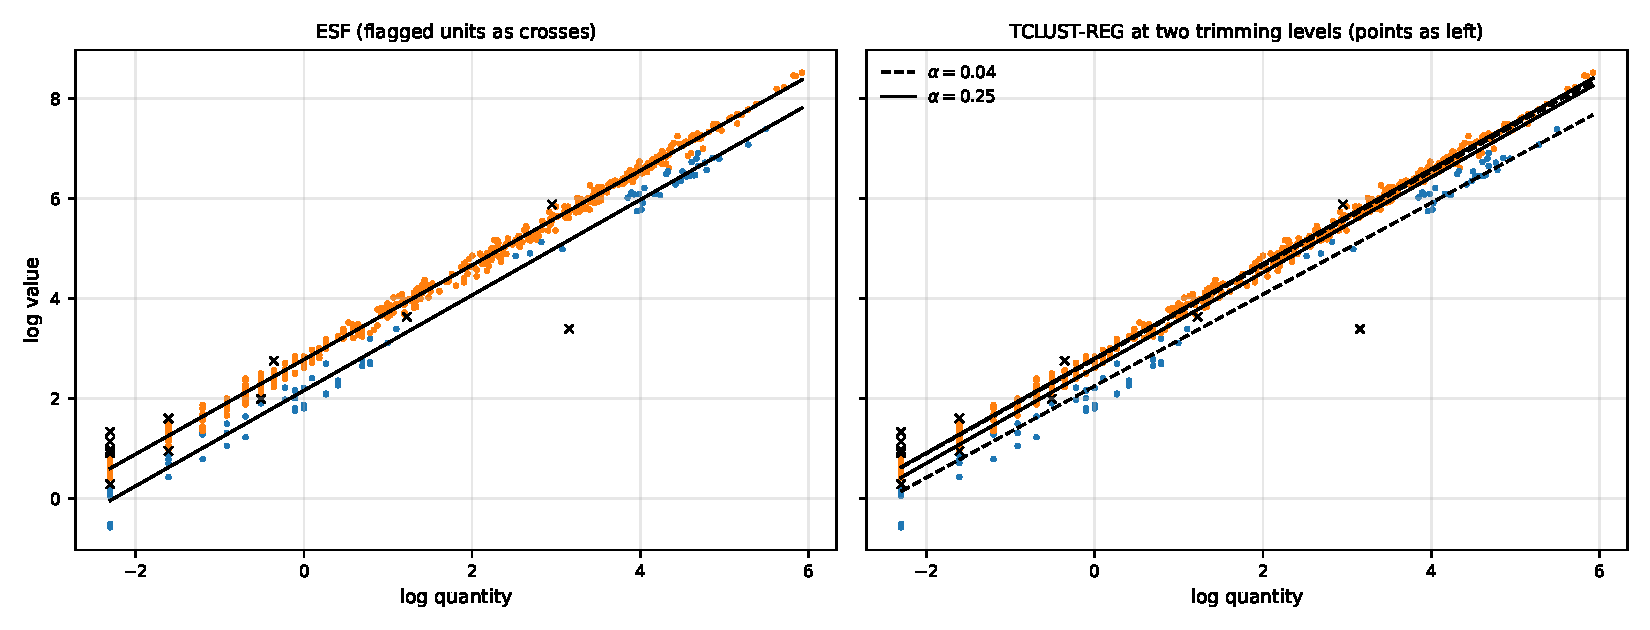
\includegraphics[width=0.9\textwidth]{figures/fishery.pdf}
\caption{Fishery data (Section~5.1 of the paper) on the logarithmic scale. Left: the two lines of ESF with the recovery
step (seed $0$), with its flagged flows as crosses and the other flows coloured by group.
Right: TCLUST-REG at trimming levels $0.04$ (dashed) and $0.25$ (solid), with the same
points.}
\label{fig:fishery}
\end{figure}

On the taxi data (Table~\ref{tab:taxi}), TLE at levels $0.10$ and $0.15$ and CTLE stopped with
an error on $18$, $19$ and $13$ of the $20$ samples; when they returned a fit, it was as
accurate as the best ($0.98$). The Laplace mixture fell below $0.7$ on $14$ samples, and least
squares on all.

\begin{table}[htbp]
\centering
\scriptsize
\caption{Fishery data (Section~5.1 of the paper), logarithmic scale, $K=2$: estimated
intercepts and slopes, median over random seeds or starts, with the range in brackets when it
exceeds $0.005$, and the trimmed or flagged fraction.}
\label{tab:fishery}
\resizebox{\textwidth}{!}{\begin{tabular}{lccc}
\toprule
Method & Group 1: intercept, slope & Group 2: intercept, slope & Trimmed or flagged \\
\midrule
ESF (20 seeds) & 2.16 [2.16, 2.58], 0.96 [0.95, 0.98] & 2.78 [2.78, 2.85], 0.94 & 0.03 [0.02, 0.12] \\
ESF alone (20 seeds) & 2.57 [2.56, 2.59], 0.98 [0.97, 0.98] & 2.85 [2.84, 2.86], 0.95 [0.94, 0.95] & 0.11 [0.10, 0.12] \\
TCLUST-REG, $\alpha=0.02$ (10 seeds) & 2.21, 0.93 & 2.78, 0.94 & 0.02 \\
TCLUST-REG, $\alpha=0.04$ (10 seeds) & 2.25, 0.92 & 2.78, 0.94 & 0.04 \\
TCLUST-REG, $\alpha=0.06$ (10 seeds) & 2.24, 0.92 & 2.78, 0.94 & 0.06 \\
TCLUST-REG, $\alpha=0.08$ (10 seeds) & 2.22 [2.22, 2.24], 0.92 & 2.78, 0.94 & 0.08 \\
TCLUST-REG, $\alpha=0.10$ (10 seeds) & 2.31 [1.91, 2.37], 0.94 [0.90, 0.99] & 2.77, 0.95 & 0.10 \\
TCLUST-REG, $\alpha=0.15$ (10 seeds) & 2.50 [1.81, 2.78], 0.94 [0.38, 0.95] & 2.79 [2.78, 2.84], 0.94 [0.79, 0.95] & 0.15 \\
TCLUST-REG, $\alpha=0.20$ (10 seeds) & 2.62 [2.56, 2.78], 0.95 [0.81, 1.07] & 2.78 [2.78, 2.80], 0.95 [0.81, 0.95] & 0.20 \\
TCLUST-REG, $\alpha=0.25$ (10 seeds) & 2.61 [2.55, 2.79], 0.96 [0.87, 1.01] & 2.79 [2.79, 2.87], 0.94 [0.84, 0.95] & 0.25 \\
TCLUST-REG, $\alpha=0.30$ (10 seeds) & 2.63 [2.55, 2.67], 0.95 [0.93, 1.03] & 2.80 [2.78, 2.82], 0.94 [0.94, 0.95] & 0.30 \\
CTLE (10 seeds) & 2.34, 0.94 & 2.79, 0.94 & 0.02 \\
Trimmed CWM, $\alpha=0.04$ (10 seeds) & 2.62 [2.28, 2.71], 0.89 [0.72, 0.97] & 2.80 [2.78, 2.80], 0.94 [0.82, 0.94] & 0.04 \\
Trimmed CWM, $\alpha=0.10$ (10 seeds) & 2.65 [2.56, 2.75], 0.96 [0.90, 1.00] & 2.78 [2.76, 2.85], 0.94 [0.83, 0.96] & 0.10 \\
Trimmed CWM, $\alpha=0.25$ (10 seeds) & 2.73 [2.57, 2.78], 0.96 [0.91, 1.00] & 2.79 [2.78, 2.84], 0.95 [0.94, 0.96] & 0.25 \\
\bottomrule
\end{tabular}}
\end{table}

\begin{table}[htbp]
\centering
\scriptsize
\caption{Taxi trips from JFK airport (Section~5.3 of the paper), $20$ random samples of
$2{,}000$ trips, $K=2$: mean and worst accuracy on the trips with rate codes 1 and 2, median
coefficient error against the flat fare ($70$, $0$, $0$) and a robust least-squares fit to all
metered trips of the month, mean flagged or trimmed fraction, and median time. A failed fit
counts as accuracy $0$. ``Reweighted'' is the rule of the paper, not that of
\citet{dotto2018reweighting}.}
\label{tab:taxi}
\resizebox{\textwidth}{!}{\begin{tabular}{lccccc}
\toprule
Method & Accuracy, mean & Accuracy, worst & Coefficient error & Flagged or trimmed & Time (s) \\
\midrule
ESF & 0.978 & 0.974 & 0.23 & 0.23 & 31 \\
ESF alone & 0.978 & 0.974 & 0.23 & 0.23 & 24 \\
TCLUST-REG (long search), $\alpha=0.25$, reweighted, then the recovery step & 0.979 & 0.975 & 0.10 & 0.14 & 86 \\
TCLUST-REG (long search), $\alpha=0.40$, reweighted, then the recovery step & 0.978 & 0.973 & 0.14 & 0.14 & 54 \\
TCLUST-REG (long search), $\alpha=0.25$, reweighted & 0.979 & 0.975 & 0.10 & 0.14 & 86 \\
TCLUST-REG (long search), $\alpha=0.40$, reweighted & 0.978 & 0.973 & 0.14 & 0.14 & 54 \\
TCLUST-REG, $\alpha=0.05$ & 0.972 & 0.959 & 0.98 & 0.05 & 7.30 \\
TCLUST-REG, $\alpha=0.10$ & 0.978 & 0.975 & 0.06 & 0.10 & 5.11 \\
TCLUST-REG, $\alpha=0.15$ & 0.978 & 0.975 & 0.09 & 0.15 & 4.35 \\
TCLUST-REG, $\alpha=0.25$ & 0.977 & 0.967 & 0.21 & 0.25 & 4.10 \\
TCLUST-REG, $\alpha=0.40$ & 0.975 & 0.965 & 0.48 & 0.40 & 3.02 \\
TCLUST-REG, $\alpha=0.25$, reweighted & 0.979 & 0.975 & 0.10 & 0.14 & 4.10 \\
TCLUST-REG, $\alpha=0.40$, reweighted & 0.978 & 0.970 & 0.13 & 0.14 & 3.02 \\
Trimmed CWM, $\alpha=0.05$ & 0.905 & 0.592 & 1.82 & 0.05 & 12 \\
Trimmed CWM, $\alpha=0.10$ & 0.978 & 0.975 & 0.06 & 0.10 & 12 \\
Trimmed CWM, $\alpha=0.15$ & 0.978 & 0.974 & 0.15 & 0.15 & 12 \\
Trimmed CWM, $\alpha=0.25$ & 0.978 & 0.970 & 0.20 & 0.25 & 11 \\
Trimmed CWM, $\alpha=0.40$ & 0.977 & 0.967 & 0.32 & 0.40 & 12 \\
TLE, $\alpha=0.05$ & 0.567 & 0.000 & 17.74 & 0.05 & 58 \\
TLE, $\alpha=0.10$ & 0.098 & 0.000 & 0.12 & 0.10 & 6.77 \\
TLE, $\alpha=0.15$ & 0.049 & 0.000 & 0.16 & 0.15 & 8.41 \\
TLE, $\alpha=0.25$ & 0.700 & 0.000 & 64.30 & 0.25 & 61 \\
TLE, $\alpha=0.40$ & 0.686 & 0.593 & 66.26 & 0.40 & 53 \\
CTLE & 0.342 & 0.000 & 0.24 & 0.09 & 80 \\
Bisquare mixture & 0.979 & 0.975 & 0.08 & 0.00 & 5.41 \\
Laplace mixture & 0.676 & 0.534 & 65.37 & 0.00 & 1136 \\
Contaminated normal mixture & 0.978 & 0.974 & 0.12 & 0.09 & 0.29 \\
Noise-component mixture & 0.978 & 0.974 & 0.23 & 0.08 & 0.04 \\
Least squares (50 starts) & 0.589 & 0.571 & 6.72 & -- & 0.07 \\
\bottomrule
\end{tabular}}
\end{table}

\begin{table}[htbp]
\centering
\scriptsize
\caption{Constants of ESF and of the recovery step (Section~2.5 of the paper), their values, the range examined, and the
largest change in a cell's mean accuracy over that range, up to $20\%$ of outliers unless
stated. For the loss cap the changes are relative to $c_{\mathrm b}=3$. S: table of this Supplement.}
\label{tab:constants}
\resizebox{\textwidth}{!}{%
\begin{tabular}{lllll}
\toprule
Constant & Value & Range examined & Change & Evidence \\
\midrule
\multicolumn{5}{l}{\emph{ESF (Algorithm~1 of the paper)}} \\
subsample size $m$ & $(d+1)/\pi_{\min}$ with room & up to $16$--$20$; $m=12$ everywhere & $0.02$; $0.035$ from $25\%$; $0.025$ (small groups); $0.07$ with four groups ($m=12$ for $16$) & S12, S15, S28, S39 \\
replicates $B$, stages $L$ & $100$, $10$ & $B=500$; $500$, $1000$ (fishery) & $-0.02$ to $+0.03$; $-0.07$ at $30\%$ & S29; Section~5.1 of the paper \\
cut-off $c$ & $2.5$ & $2$ to $3$ & $0.024$; $0.04$ at $30\%$ & S3 \\
loss cap $c_{\mathrm b}$ & $3$ & $3$ to $5$ & $0.13$ lost at $5$ (D5); $0.24$ gained with a group of $15\%$ & S13 \\
vote weight $\lambda$ & $3$ & $0$, $\infty$ & $0.05$ at $\lambda=0$ & S2 \\
covariate quantile & $0.975$ & $0.95$ to $0.99$ & $0.007$; $0.015$ at $30\%$; $0.21$ with leverage points & S3 \\
minimum group for screen & $\max(10,5p)$ & -- & -- & -- \\
\multicolumn{5}{l}{\emph{Recovery step (Algorithm~2 of the paper)}} \\
peak weight & $\tfrac12$ & $0.4$, $0.6$ & $0.015$ & S23 \\
window & $3c$ scales & $2c$, $4c$ & $0.03$ & S23 \\
minimum support & $\max\{2(d+1),0.03n\}$ & $0.02n$, $0.05n$ & $0.026$ & S23 \\
restriction factor & $12$ & $8$, $20$ & $0.016$ & S23 \\
margin & $\tfrac{d+1}{2}\log n$ & halved, doubled & $0.016$ & S23 \\
limit on flagged fraction & $n/3$ & $0.25n$, $0.40n$ & $0.20$ at $0.25n$ & S23 \\
noise range, random lines, applications & $1.1\,\mathrm{range}(y)$, $500$, $3$ & -- & -- & -- \\
\bottomrule
\end{tabular}}
\end{table}

\begin{table}[htbp]
\centering
\footnotesize
\caption{Criteria that count flagged or trimmed clean units (descriptive; Section~4.1 of the
paper), over the same $123$ cells as Table~2 of the paper: the adjusted Rand index on all units,
with the outliers as a class of their own and every flagged or trimmed unit labelled as an
outlier, and the misclassification rate of the clean units, counting a flagged clean unit as an
error (the labels matched to the true groups by the best permutation). Flags are those of the
reweighting rule ($c=2.5$), with the covariate screen for ESF and without it for TCLUST-REG.
Mean over cells of the cell means, and the worst cell. rw: the reweighting step; recovery:
followed by the recovery step.}
\label{tab:S45}
\resizebox{\textwidth}{!}{\begin{tabular}{lcccccccc}
\toprule
 & \multicolumn{4}{c}{$\varepsilon\le0.20$ (89 cells)} & \multicolumn{4}{c}{$\varepsilon\ge0.25$ (34 cells)} \\
\cmidrule(lr){2-5}\cmidrule(lr){6-9}
Method & ARI mean & ARI worst & Misc.\ mean & Misc.\ worst & ARI mean & ARI worst & Misc.\ mean & Misc.\ worst \\
\midrule
ESF & 0.719 & 0.54 & 0.102 & 0.29 & 0.660 & 0.01 & 0.183 & 0.48 \\
TCLUST-REG, $\alpha=0.25$, rw, recovery & 0.725 & 0.57 & 0.096 & 0.17 & 0.519 & 0.00 & 0.308 & 0.49 \\
TCLUST-REG, $\alpha=0.40$, rw, recovery & 0.715 & 0.56 & 0.104 & 0.19 & 0.714 & 0.01 & 0.138 & 0.48 \\
TCLUST-REG, $\alpha=0.25$, rw & 0.694 & 0.26 & 0.127 & 0.45 & 0.521 & 0.00 & 0.306 & 0.49 \\
TCLUST-REG, $\alpha=0.40$, rw & 0.624 & 0.24 & 0.201 & 0.52 & 0.720 & 0.02 & 0.133 & 0.47 \\
\bottomrule
\end{tabular}}
\end{table}

\begin{table}[htbp]
\centering
\footnotesize
\caption{The recovery step after the trimmed cluster-weighted model (descriptive;
Section~4.6 of the paper): mean over cells of the mean accuracy on clean units, the number of
cells with a mean below $0.85$, and the worst cell, over the same $123$ cells as Table~2 of the
paper. The model is fitted by RobMixReg at levels $0.25$ and $0.40$ ($50$ starts), then
reweighted by our rule (rw) and followed by the recovery step.}
\label{tab:S46}
\resizebox{\textwidth}{!}{\begin{tabular}{lcccccc}
\toprule
 & \multicolumn{3}{c}{$\varepsilon\le0.20$ (89 cells)} & \multicolumn{3}{c}{$\varepsilon\ge0.25$ (34 cells)} \\
\cmidrule(lr){2-4}\cmidrule(lr){5-7}
Method & Mean & Below $0.85$ & Worst & Mean & Below $0.85$ & Worst \\
\midrule
Trimmed CWM, $\alpha=0.25$, alone & 0.786 & 47 & 0.57 & 0.677 & 32 & 0.53 \\
Trimmed CWM, $\alpha=0.25$, rw & 0.804 & 39 & 0.56 & 0.682 & 32 & 0.53 \\
Trimmed CWM, $\alpha=0.25$, rw, recovery & 0.882 & 12 & 0.66 & 0.679 & 31 & 0.53 \\
Trimmed CWM, $\alpha=0.40$, alone & 0.716 & 77 & 0.56 & 0.759 & 28 & 0.58 \\
Trimmed CWM, $\alpha=0.40$, rw & 0.745 & 66 & 0.54 & 0.786 & 24 & 0.61 \\
Trimmed CWM, $\alpha=0.40$, rw, recovery & 0.871 & 20 & 0.64 & 0.785 & 24 & 0.62 \\
\bottomrule
\end{tabular}}
\end{table}

\begin{table}[htbp]
\centering
\scriptsize
\caption{The five analysis plans (Section~4.1 of the paper): what each fixed before the data it concerns were analysed
(Plans~1 and~2) or generated (Plans~3 to~5), and the data it concerns. The third part of the
study ($2{,}300$ data sets) is descriptive and had no plan.}
\label{tab:plans}
\begin{tabular}{@{}lp{6.5cm}p{5.0cm}@{}}
\toprule
Plan & What it fixed & Data it concerns \\
\midrule
1 & ESF alone against the best competitor chosen after the run in each cell: mean paired
difference not below $-0.03$, upper $95\%$ bound not below $-0.02$; every fixed-level
competitor to fall $0.05$ below ESF alone somewhere & First part: D1 to D8,
$\varepsilon\in\{0,0.05,0.10,0.20,0.30\}$, $50$ data sets per cell, $2{,}000$; the comparison
concerns $\varepsilon\le0.20$ \\
2 & Whether TCLUST-REG at level $0.25$ with reweighting fails above its level while ESF alone
does not (gap of $0.05$, interval excluding zero, in some design without high-leverage points)
& Second part: $\varepsilon\in\{0.25,0.30,0.35\}$, new data, $100$ per cell, $2{,}400$ \\
3 & The recovery step, code frozen: gain of at least $0.05$ in the small-group cells, no loss
above $0.01$ at $\varepsilon\le0.20$, the comparison of Plan~1 for ESF with the step & The
stored fits of ESF alone on the $6{,}400$ data sets of the first three parts \\
4 & The same confirmation on fresh data & $600$ new data sets in four small-group designs \\
5 & The comparison of Plan~1 in three designs outside the Gaussian family & $450$ new data sets \\
\bottomrule
\end{tabular}
\end{table}

\begin{table}[htbp]
\centering
\footnotesize
\caption{Sensitivity of the recovery step to its noise range (descriptive; Section~4.6 of the
paper): the range $R$, $1.1$ times the range of the response, multiplied by $2$ and $5$, as if
the most extreme unit lay two or five times farther out, and replaced by two ranges tied to the
fitted scales ($20$ median group scales; the range of the unflagged units plus $10$ median
scales); mean over cells of the mean accuracy
on clean units, the number of cells with a mean below $0.85$, and the worst cell, over the same
$123$ cells as Table~2 of the paper. Fits and seeds as in the study.}
\label{tab:S48}
\resizebox{\textwidth}{!}{\begin{tabular}{lcccccc}
\toprule
 & \multicolumn{3}{c}{$\varepsilon\le0.20$ (89 cells)} & \multicolumn{3}{c}{$\varepsilon\ge0.25$ (34 cells)} \\
\cmidrule(lr){2-4}\cmidrule(lr){5-7}
Method & Mean & Below $0.85$ & Worst & Mean & Below $0.85$ & Worst \\
\midrule
ESF, range $R$ as in the paper & 0.914 & 2 & 0.78 & 0.820 & 13 & 0.53 \\
ESF, range $2R$ & 0.912 & 2 & 0.69 & 0.812 & 15 & 0.53 \\
ESF, range $5R$ & 0.910 & 3 & 0.68 & 0.799 & 16 & 0.53 \\
ESF, range $20$ median scales & 0.891 & 12 & 0.62 & 0.819 & 13 & 0.53 \\
ESF, unflagged range plus $10$ median scales & 0.903 & 9 & 0.70 & 0.817 & 13 & 0.53 \\
TCLUST-REG $0.40$, rw, recovery, range $R$ & 0.909 & 4 & 0.81 & 0.863 & 8 & 0.53 \\
TCLUST-REG $0.40$, rw, recovery, range $2R$ & 0.908 & 5 & 0.81 & 0.846 & 10 & 0.54 \\
TCLUST-REG $0.40$, rw, recovery, range $5R$ & 0.906 & 7 & 0.75 & 0.830 & 12 & 0.54 \\
TCLUST-REG $0.40$, rw, recovery, $20$ median scales & 0.883 & 15 & 0.61 & 0.859 & 9 & 0.54 \\
TCLUST-REG $0.40$, rw, recovery, unflagged range plus $10$ scales & 0.899 & 10 & 0.73 & 0.853 & 9 & 0.54 \\
\bottomrule
\end{tabular}}
\end{table}

\begin{table}[htbp]
\centering
\footnotesize
\caption{TCLUST-REG's own assignment against the criterion of the paper (descriptive;
Section~4.1 of the paper): mean accuracy on clean units of the long-search fits at levels $0.25$
and $0.40$ (without reweighting) when every clean unit takes the label of its nearest fitted line,
as in the paper, and when it takes the label that TCLUST-REG assigns (\texttt{out.idx}), trimmed
clean units then taking that of their nearest line; and the fraction of clean units trimmed.
Same fits and data sets as the study.}
\label{tab:S49}
\resizebox{\textwidth}{!}{\begin{tabular}{llcccccc}
\toprule
 & & \multicolumn{3}{c}{$\alpha=0.25$} & \multicolumn{3}{c}{$\alpha=0.40$} \\
\cmidrule(lr){3-5}\cmidrule(lr){6-8}
Design & $\varepsilon$ & Nearest line & Own assignment & Clean trimmed & Nearest line & Own assignment & Clean trimmed \\
\midrule
D2 & 0.00 & 0.876 & 0.868 & 0.250 & 0.794 & 0.792 & 0.400 \\
D2 & 0.05 & 0.883 & 0.874 & 0.213 & 0.830 & 0.829 & 0.371 \\
D2 & 0.10 & 0.891 & 0.878 & 0.165 & 0.841 & 0.837 & 0.332 \\
D2 & 0.20 & 0.883 & 0.861 & 0.065 & 0.840 & 0.832 & 0.251 \\
D4 & 0.00 & 0.911 & 0.917 & 0.250 & 0.908 & 0.916 & 0.400 \\
D4 & 0.05 & 0.908 & 0.914 & 0.210 & 0.905 & 0.911 & 0.368 \\
D4 & 0.10 & 0.909 & 0.918 & 0.167 & 0.907 & 0.912 & 0.333 \\
D4 & 0.20 & 0.907 & 0.925 & 0.066 & 0.905 & 0.911 & 0.252 \\
D2 & 0.25 & 0.756 & 0.735 & 0.018 & 0.857 & 0.847 & 0.195 \\
D2 & 0.30 & 0.618 & 0.604 & 0.005 & 0.859 & 0.838 & 0.141 \\
D2 & 0.35 & 0.507 & 0.497 & 0.002 & 0.834 & 0.801 & 0.076 \\
D4 & 0.25 & 0.875 & 0.896 & 0.013 & 0.911 & 0.917 & 0.199 \\
D4 & 0.30 & 0.617 & 0.621 & 0.004 & 0.910 & 0.918 & 0.140 \\
D4 & 0.35 & 0.530 & 0.531 & 0.003 & 0.911 & 0.926 & 0.072 \\
$K=4$ & 0.00 & 0.925 & 0.929 & 0.250 & 0.792 & 0.809 & 0.400 \\
$K=4$ & 0.10 & 0.932 & 0.932 & 0.168 & 0.794 & 0.809 & 0.334 \\
$K=4$ & 0.20 & 0.896 & 0.884 & 0.068 & 0.795 & 0.805 & 0.256 \\
$K=4$ & 0.30 & 0.748 & 0.749 & 0.004 & 0.758 & 0.756 & 0.150 \\
\bottomrule
\end{tabular}}
\end{table}

\begin{table}[htbp]
\centering
\footnotesize
\caption{The eleven cells that decide the comparison up to $20\%$ of outliers, with $200$ data
sets each: the $50$ of the study and $150$ further ones from the same generators (descriptive;
Section~4.2 of the paper). Mean accuracy on clean units of ESF with its standard error, and, for
TCLUST-REG with the long search, reweighting and the recovery step at level $0.25$, at level
$0.30$ and at level $0.25$ with equal weights, the mean and the paired difference ESF minus that
pipeline with its standard error.}
\label{tab:S50}
\resizebox{\textwidth}{!}{\begin{tabular}{llcccccccc}
\toprule
Design & $\varepsilon$ & $n_{\mathrm{rep}}$ & ESF & \multicolumn{2}{c}{$0.25$} & \multicolumn{2}{c}{$0.30$} & \multicolumn{2}{c}{$0.25$, equal weights} \\
\cmidrule(lr){5-6}\cmidrule(lr){7-8}\cmidrule(lr){9-10}
 & & & mean (s.e.) & mean & ESF $-$ (s.e.) & mean & ESF $-$ (s.e.) & mean & ESF $-$ (s.e.) \\
\midrule
D2 & 0.00 & 200 & 0.905 (0.001) & 0.889 & +0.016 (0.003) & 0.876 & +0.029 (0.005) & 0.897 & +0.008 (0.002) \\
D2 & 0.05 & 200 & 0.903 (0.002) & 0.893 & +0.010 (0.003) & 0.886 & +0.017 (0.004) & 0.899 & +0.004 (0.002) \\
D2 & 0.10 & 200 & 0.899 (0.003) & 0.899 & -0.000 (0.003) & 0.889 & +0.009 (0.004) & 0.900 & -0.002 (0.003) \\
D2 & 0.20 & 200 & 0.904 (0.003) & 0.891 & +0.012 (0.004) & 0.901 & +0.003 (0.003) & 0.906 & -0.003 (0.002) \\
$K=4$ & 0.00 & 200 & 0.961 (0.002) & 0.929 & +0.032 (0.006) & 0.901 & +0.060 (0.007) & 0.963 & -0.002 (0.002) \\
$K=4$ & 0.10 & 200 & 0.959 (0.002) & 0.923 & +0.036 (0.006) & 0.898 & +0.061 (0.007) & 0.962 & -0.003 (0.002) \\
$K=4$ & 0.20 & 200 & 0.945 (0.005) & 0.901 & +0.044 (0.008) & 0.888 & +0.058 (0.008) & 0.955 & -0.010 (0.005) \\
80/20 & 0.20 & 200 & 0.883 (0.007) & 0.910 & -0.027 (0.007) & 0.909 & -0.026 (0.007) & 0.909 & -0.026 (0.007) \\
clustered & 0.20 & 200 & 0.810 (0.012) & 0.904 & -0.094 (0.012) & 0.909 & -0.100 (0.012) & 0.910 & -0.100 (0.012) \\
80/20, $p=3$ & 0.20 & 200 & 0.850 (0.009) & 0.907 & -0.057 (0.009) & 0.896 & -0.046 (0.010) & 0.900 & -0.050 (0.009) \\
85/15, parallel & 0.20 & 200 & 0.880 (0.013) & 0.967 & -0.088 (0.011) & 0.962 & -0.083 (0.011) & 0.964 & -0.085 (0.011) \\
\bottomrule
\end{tabular}}
\end{table}

\clearpage
\section*{S7 Implementation of ESF}
\label{app:implementation}

\paragraph{Exact subsample fits.}
Label vectors are enumerated depth first in restricted-growth form: unit $j$ may receive any
label already used by units $1,\dots,j-1$ or the smallest unused one. This lists each
partition into at most $K$ groups exactly once and removes the $K!$ relabellings. Each group
keeps its sufficient statistics $(n_k,X_k^{\top}X_k,X_k^{\top}y_k,y_k^{\top}y_k)$, updated in
$O(d^{2})$ when a unit enters or leaves, and its residual sum of squares, recomputed by a
Cholesky solve of size $d$. For rank-deficient groups the minimum-norm solution is used; its
residual sum of squares is the minimum over all coefficient vectors, so the group criterion is
exact in every case. A group's residual sum of squares cannot decrease when a unit is added,
so the sum over groups at a partial labelling is a lower bound for every completion, and a
branch is abandoned when the bound reaches the best value found. The cost of the search is reported in Section~2.2 of the paper and in Table~S30.

The code was
checked against plain enumeration of all $K^{m}$ label vectors, with residual sums of squares
computed independently by a least-squares routine, on $200$ instances with $(K,d,m)$ equal
to $(2,1,10)$, $(2,2,10)$, $(3,2,8)$ or $(2,3,9)$, a third of them with tied covariates.

\paragraph{Scoring scale.} The scale $s$ of the bounded loss (Algorithm~1 of the paper, line~5) is the smallest, over the replicates, of the median
squared residual over all unflagged units divided by $0.4549$, the median of $\chi^{2}_1$: for a
replicate that fits the clean majority this is a rough estimate of the error variance. The
minimum is biased downwards by design: the cap should follow the best replicate, not a
typical one.

\paragraph{Alignment and vote.}
Replicates are aligned before voting by solving an assignment problem between their coefficients
and those of a common reference, by enumerating the $K!$ relabellings for $K\le6$, which covers
every experiment here (the Hungarian method \citep{kuhn1955hungarian} is used beyond). The
reference is a pilot replicate, the best of ten preliminary replicates by the median of the
squared residuals; it serves only for alignment and does not vote. After the vote, a group with
fewer than $d$ unflagged units keeps the coefficients of the best-scoring replicate $b^{\ast}$ of
the last stage. The final reweighting step recomputes the flags at the current fit and refits
each group on its unflagged units.

\paragraph{Concentration steps.}
Every unit is assigned to its nearest surface, the $h$ units with the smallest squared
residuals are kept, and each group is refitted on its kept units; this is repeated until the
trimmed sum of squares stops decreasing, at most $200$ times.

\paragraph{Software.}
ESF and the recovery step are written in Python with \texttt{numpy}, \texttt{scipy} and \texttt{numba}, and
the covariate screen uses the minimum covariance determinant of \texttt{scikit-learn} when
there is more than one covariate. The code, the scripts that produce every table and figure,
and the raw results are at \url{https://github.com/sorujov/eesp}.

\begin{table}[htbp]
\centering
\footnotesize
\caption{TCLUST-REG in MATLAB and in Octave (Section~S1) on the same $80$ data sets, ten per cell, with
$1000$ starts and $50$ refinement steps. Same fit: fits with the same coefficients (of $10$).
MATLAB, Octave: mean accuracy after reweighting and the recovery step. MATLAB higher, Octave
higher: fits whose score (see the text) exceeds the other program's by more than $0.5$.}
\label{tab:matlab}
\begin{tabular}{llcccccc}
\toprule
Design & $\varepsilon$ & $\alpha$ & Same fit & MATLAB & Octave & MATLAB higher & Octave higher \\
\midrule
D1 & 0.10 & 0.25 & 9 & 0.922 & 0.922 & 0 & 0 \\
D1 & 0.10 & 0.40 & 3 & 0.923 & 0.923 & 0 & 0 \\
D2 & 0.10 & 0.25 & 2 & 0.901 & 0.901 & 4 & 0 \\
D2 & 0.10 & 0.40 & 0 & 0.847 & 0.843 & 4 & 3 \\
D2 & 0.20 & 0.25 & 3 & 0.917 & 0.918 & 1 & 2 \\
D2 & 0.20 & 0.40 & 0 & 0.884 & 0.823 & 5 & 4 \\
D5 & 0.20 & 0.25 & 10 & 0.832 & 0.832 & 0 & 0 \\
D5 & 0.20 & 0.40 & 6 & 0.874 & 0.832 & 1 & 0 \\
D6 & 0.20 & 0.25 & 10 & 0.904 & 0.904 & 0 & 0 \\
D6 & 0.20 & 0.40 & 8 & 0.908 & 0.908 & 0 & 0 \\
D2 & 0.30 & 0.25 & 0 & 0.551 & 0.499 & 4 & 3 \\
D2 & 0.30 & 0.40 & 0 & 0.799 & 0.831 & 2 & 6 \\
D6 & 0.35 & 0.25 & 8 & 0.685 & 0.685 & 0 & 0 \\
D6 & 0.35 & 0.40 & 9 & 0.692 & 0.692 & 0 & 0 \\
$K=4$ & 0.10 & 0.25 & 0 & 0.958 & 0.895 & 3 & 7 \\
$K=4$ & 0.10 & 0.40 & 0 & 0.772 & 0.866 & 4 & 5 \\
\midrule
All & & & 68 & 0.836 & 0.830 & 28 & 30 \\
\bottomrule
\end{tabular}
\end{table}

\begin{thebibliography}{99}
\small
\bibitem[Bagirov et al.(2013)]{bagirov2013nonsmooth} Bagirov, A. M., Ugon, J., \& Mirzayeva, H. (2013). Nonsmooth nonconvex optimization approach to clusterwise linear regression problems. \textit{European Journal of Operational Research}, 229(1), 132--142.

\bibitem[Bai et al.(2012)]{bai2012robust} Bai, X., Yao, W., \& Boyer, J. E. (2012). Robust fitting of mixture regression models. \textit{Computational Statistics \& Data Analysis}, 56(7), 2347--2359.

\bibitem[Banfield \& Raftery(1993)]{banfield1993model} Banfield, J. D., \& Raftery, A. E. (1993). Model-based Gaussian and non-Gaussian clustering. \textit{Biometrics}, 49(3), 803--821.

\bibitem[Benaglia et al.(2009)]{benaglia2009mixtools} Benaglia, T., Chauveau, D., Hunter, D. R., \& Young, D. S. (2009). mixtools: an R package for analyzing finite mixture models. \textit{Journal of Statistical Software}, 32(6), 1--29.

\bibitem[Bertsimas \& Shioda(2007)]{bertsimas2007classification} Bertsimas, D., \& Shioda, R. (2007). Classification and regression via integer optimization. \textit{Operations Research}, 55(2), 252--271.

\bibitem[Brusco(2006)]{brusco2006repetitive} Brusco, M. J. (2006). A repetitive branch-and-bound procedure for minimum within-cluster sums of squares partitioning. \textit{Psychometrika}, 71(2), 347--363.

\bibitem[Cao et al.(2026)]{cao2026robmixreg} Cao, S., Chang, W., \& Zhang, C. (2026). \textit{RobMixReg: Robust Mixture Regression}. R package version 1.1.3, published on CRAN 2 June 2026. doi:10.32614/CRAN.package.RobMixReg.

\bibitem[Carbonneau et al.(2011)]{carbonneau2011globally} Carbonneau, R. A., Caporossi, G., \&
Hansen, P. (2011). Globally optimal clusterwise regression by mixed logical-quadratic
programming. \textit{European Journal of Operational Research}, 212(1), 213--222.

\bibitem[Carbonneau et al.(2012)]{carbonneau2012extensions} Carbonneau, R. A., Caporossi, G.,
\& Hansen, P. (2012). Extensions to the repetitive branch and bound algorithm for globally
optimal clusterwise regression. \textit{Computers \& Operations Research}, 39(11),
2748--2762.

\bibitem[Carbonneau et al.(2014)]{carbonneau2014globally} Carbonneau, R. A., Caporossi, G., \& Hansen, P. (2014). Globally optimal clusterwise regression by column generation enhanced with heuristics, sequencing and ending subset optimization. \textit{Journal of Classification}, 31(2), 219--241.

\bibitem[Cerioli et al.(2018)]{cerioli2018finding} Cerioli, A., Garc\'{\i}a-Escudero, L. A., Mayo-Iscar, A., \& Riani, M. (2018). Finding the number of normal groups in model-based clustering via constrained likelihoods. \textit{Journal of Computational and Graphical Statistics}, 27(2), 404--416.

\bibitem[Cerioli \& Perrotta(2014)]{cerioli2014robust} Cerioli, A., \& Perrotta, D. (2014). Robust clustering around regression lines with high density regions. \textit{Advances in Data Analysis and Classification}, 8(1), 5--26.

\bibitem[Chang et al.(2020)]{chang2020componentwise} Chang, W., Zhou, X., Zang, Y., Zhang, C., \& Cao, S. (2020). Component-wise adaptive trimming for robust mixture regression. arXiv preprint arXiv:2005.11599.

\bibitem[DeSarbo \& Cron(1988)]{desarbo1988maximum} DeSarbo, W. S., \& Cron, W. L. (1988). A
maximum likelihood methodology for clusterwise linear regression. \textit{Journal of
Classification}, 5(2), 249--282.

\bibitem[De Veaux(1989)]{deveaux1989mixtures} De Veaux, R. D. (1989). Mixtures of linear regressions. \textit{Computational Statistics \& Data Analysis}, 8(3), 227--245.

\bibitem[Dotto et al.(2018)]{dotto2018reweighting} Dotto, F., Farcomeni, A.,
Garc\'{\i}a-Escudero, L. A., \& Mayo-Iscar, A. (2018). A reweighting approach to robust
clustering. \textit{Statistics and Computing}, 28(2), 477--493.

\bibitem[Fischler \& Bolles(1981)]{fischler1981random} Fischler, M. A., \& Bolles, R. C. (1981). Random sample consensus: a paradigm for model fitting with applications to image analysis and automated cartography. \textit{Communications of the ACM}, 24(6), 381--395.

\bibitem[Fois et al.(2026)]{fois2026clusterwise} Fois, A., Insolia, L., Consolini, L., Laurini, F., Locatelli, M., \& Riani, M. (2026). Clusterwise linear regression using a probabilistic branch and bound algorithm under Gaussianity. \textit{Computers \& Operations Research}, 189, 107375.

\bibitem[Garc\'{\i}a-Escudero et al.(2009)]{garciaescudero2009robust} Garc\'{\i}a-Escudero, L. A., Gordaliza, A., San Mart\'{\i}n, R., Van Aelst, S., \& Zamar, R. (2009). Robust linear clustering. \textit{Journal of the Royal Statistical Society Series B}, 71(1), 301--318.

\bibitem[Garc\'{\i}a-Escudero et al.(2010)]{garciaescudero2010robust}
Garc\'{\i}a-Escudero, L. A., Gordaliza, A., Mayo-Iscar, A., \& San Mart\'{\i}n, R. (2010).
Robust clusterwise linear regression through trimming. \textit{Computational Statistics \&
Data Analysis}, 54(12), 3057--3069.

\bibitem[Garc\'{\i}a-Escudero et al.(2011)]{garciaescudero2011exploring} Garc\'{\i}a-Escudero, L. A., Gordaliza, A., Matr\'{a}n, C., \& Mayo-Iscar, A. (2011). Exploring the number of groups in robust model-based clustering. \textit{Statistics and Computing}, 21(4), 585--599.

\bibitem[Garc\'{\i}a-Escudero et al.(2017)]{garciaescudero2017robust} Garc\'{\i}a-Escudero, L. A., Gordaliza, A., Greselin, F., Ingrassia, S., \& Mayo-Iscar, A. (2017). Robust estimation of mixtures of regressions with random covariates, via trimming and constraints. \textit{Statistics and Computing}, 27(2), 377--402.

\bibitem[Gervini \& Yohai(2002)]{gervini2002class} Gervini, D., \& Yohai, V. J. (2002). A class
of robust and fully efficient regression estimators. \textit{The Annals of Statistics}, 30(2),
583--616.

\bibitem[Gurobi Optimization(2026)]{gurobi2026} Gurobi Optimization, LLC (2026). \textit{Gurobi Optimizer Reference Manual}, version 13.0. https://www.gurobi.com.

\bibitem[Joki et al.(2020)]{joki2020clusterwise} Joki, K., Bagirov, A. M., Karmitsa, N., M\"{a}kel\"{a}, M. M., \& Taheri, S. (2020). Clusterwise support vector linear regression. \textit{European Journal of Operational Research}, 287(1), 19--35.

\bibitem[Kuhn(1955)]{kuhn1955hungarian} Kuhn, H. W. (1955). The Hungarian method for the
assignment problem. \textit{Naval Research Logistics Quarterly}, 2(1--2), 83--97.

\bibitem[Magri \& Fusiello(2014)]{magri2014tlinkage} Magri, L., \& Fusiello, A. (2014). T-linkage: a continuous relaxation of J-linkage for multi-model fitting. In \textit{2014 IEEE Conference on Computer Vision and Pattern Recognition} (pp. 3954--3961).

\bibitem[Magri \& Fusiello(2015)]{magri2015robust} Magri, L., \& Fusiello, A. (2015). Robust multiple model fitting with preference analysis and low-rank approximation. In \textit{Proceedings of the British Machine Vision Conference 2015} (pp. 20.1--20.12). BMVA Press.

\bibitem[Maher et al.(2016)]{maher2016pyscipopt} Maher, S., Miltenberger, M., Pedroso, J. P., Rehfeldt, D., Schwarz, R., \& Serrano, F. (2016). PySCIPOpt: mathematical programming in Python with the SCIP Optimization Suite. In \textit{Mathematical Software -- ICMS 2016}, Lecture Notes in Computer Science 9725 (pp. 301--307). Cham: Springer.

\bibitem[Mazza \& Punzo(2020)]{mazza2020mixtures} Mazza, A., \& Punzo, A. (2020). Mixtures of multivariate contaminated normal regression models. \textit{Statistical Papers}, 61(2), 787--822.

\bibitem[Megiddo \& Tamir(1982)]{megiddo1982complexity} Megiddo, N., \& Tamir, A. (1982). On the complexity of locating linear facilities in the plane. \textit{Operations Research Letters}, 1(5), 194--197.

\bibitem[Neykov et al.(2007)]{neykov2007robust} Neykov, N., Filzmoser, P., Dimova, R., \&
Neytchev, P. (2007). Robust fitting of mixtures using the trimmed likelihood estimator.
\textit{Computational Statistics \& Data Analysis}, 52(1), 299--308.

\bibitem[NYC Taxi and Limousine Commission(2024)]{tlc2024trip} NYC Taxi and Limousine Commission (2024). \textit{TLC Trip Record Data}: yellow taxi trip records, March 2024. https://www.nyc.gov/site/tlc/about/tlc-trip-record-data.page (accessed 27 September 2026).

\bibitem[Park et al.(2017)]{park2017algorithms} Park, Y. W., Jiang, Y., Klabjan, D., \& Williams, L. (2017). Algorithms for generalized clusterwise linear regression. \textit{INFORMS Journal on Computing}, 29(2), 301--317.

\bibitem[Perrotta et al.(2009)]{perrotta2009new} Perrotta, D., Riani, M., \& Torti, F. (2009). New robust dynamic plots for regression mixture detection. \textit{Advances in Data Analysis and Classification}, 3(3), 263--279.

\bibitem[Pollard(1981)]{pollard1981strong} Pollard, D. (1981). Strong consistency of
$k$-means clustering. \textit{The Annals of Statistics}, 9(1), 135--140.

\bibitem[Punzo \& McNicholas(2017)]{punzo2017robust} Punzo, A., \& McNicholas, P. D. (2017). Robust clustering in regression analysis via the contaminated Gaussian cluster-weighted model. \textit{Journal of Classification}, 34, 249--293.

\bibitem[Quandt(1972)]{quandt1972switching} Quandt, R. E. (1972). A new approach to
estimating switching regressions. \textit{Journal of the American Statistical Association},
67(338), 306--310.

\bibitem[Riani et al.(2008)]{riani2008fitting} Riani, M., Cerioli, A., Atkinson, A. C., Perrotta, D., \& Torti, F. (2008). Fitting mixtures of regression lines with the forward search. In F. Fogelman-Souli\'{e} et al. (Eds.), \textit{Mining Massive Data Sets for Security} (pp. 271--286). Amsterdam: IOS Press.

\bibitem[Riani et al.(2012)]{riani2012fsda} Riani, M., Perrotta, D., \& Torti, F. (2012). FSDA: A MATLAB toolbox for robust analysis and interactive data exploration. \textit{Chemometrics and Intelligent Laboratory Systems}, 116, 17--32.

\bibitem[Rousseeuw(1984)]{rousseeuw1984least} Rousseeuw, P. J. (1984). Least median of squares
regression. \textit{Journal of the American Statistical Association}, 79(388), 871--880.

\bibitem[Rousseeuw \& Leroy(1987)]{rousseeuw1987robust} Rousseeuw, P. J., \& Leroy, A. M.
(1987). \textit{Robust Regression and Outlier Detection}. New York: Wiley.

\bibitem[Rousseeuw \& Van Driessen(1999)]{rousseeuw1999fast} Rousseeuw, P. J., \& Van Driessen, K. (1999). A fast algorithm for the minimum covariance determinant estimator. \textit{Technometrics}, 41(3), 212--223.

\bibitem[Rousseeuw \& Van Driessen(2006)]{rousseeuw2006computing} Rousseeuw, P. J., \& Van
Driessen, K. (2006). Computing LTS regression for large data sets. \textit{Data Mining and
Knowledge Discovery}, 12(1), 29--45.

\bibitem[Song et al.(2014)]{song2014robust} Song, W., Yao, W., \& Xing, Y. (2014). Robust mixture regression model fitting by Laplace distribution. \textit{Computational Statistics \& Data Analysis}, 71, 128--137.

\bibitem[Sp\"ath(1979)]{spath1979algorithm} Sp\"ath, H. (1979). Algorithm 39: Clusterwise
linear regression. \textit{Computing}, 22(4), 367--373.

\bibitem[Toldo \& Fusiello(2008)]{toldo2008robust} Toldo, R., \& Fusiello, A. (2008). Robust multiple structures estimation with J-linkage. In \textit{Computer Vision -- ECCV 2008}, Lecture Notes in Computer Science 5302 (pp. 537--547). Berlin: Springer.

\bibitem[Torti et al.(2019)]{torti2019assessing} Torti, F., Perrotta, D., Riani, M., \& Cerioli, A. (2019). Assessing trimming methodologies for clustering linear regression data. \textit{Advances in Data Analysis and Classification}, 13(1), 227--257.

\bibitem[Torti et al.(2021)]{torti2021semiautomatic} Torti, F., Riani, M., \& Morelli, G. (2021). Semiautomatic robust regression clustering of international trade data. \textit{Statistical Methods \& Applications}, 30(3), 863--894.

\bibitem[Yao et al.(2014)]{yao2014robust} Yao, W., Wei, Y., \& Yu, C. (2014). Robust mixture regression using the $t$-distribution. \textit{Computational Statistics \& Data Analysis}, 71, 116--127.

\bibitem[Yu et al.(2017)]{yu2017new} Yu, C., Yao, W., \& Chen, K. (2017). A new method for robust mixture regression. \textit{Canadian Journal of Statistics}, 45(1), 77--94.
\end{thebibliography}

\end{document}
